\documentclass[12pt]{amsart}
%%%%%%%%%%%%%%%%%%%%%%%%%%%%%%%%%%%%%%%%%%%%%%%%%%%%%%%%%%%%%%%%%%%%%%%%%%%%%%%%%%%%%%%%%%%%%%%%%%%%%%%%%%%%%%%%%%%%%%%%%%%%%%%%%%%%%%%%%%%%%%%%%%%%%%%%%%%%%%%%%%%%%%%%%%%%%%%%%%%%%%%%%%%%%%%%%%%%%%%%%%%%%%%%%%%%%%%%%%%%%%%%%%%%%%%%%%%%%%%%%%%%%%%%%%%%   
\usepackage{amssymb}
\usepackage{amsmath}  
\usepackage{amsfonts} 
\usepackage{mathrsfs}          
\usepackage{graphicx}        
\usepackage{color}   
\usepackage[onehalfspacing]{setspace}
\usepackage{ragged2e}  
\justifying     
\usepackage{caption} 
\usepackage{etex} 
\usepackage{longtable}    
\usepackage{graphicx} 
\usepackage{amsmath}
\usepackage{multirow}
\usepackage{setspace}
\usepackage{footmisc}
\usepackage{amssymb}  
\usepackage{amsfonts}
\usepackage[font=bf, justification=centering]{caption}
\usepackage{geometry}
\usepackage{float}
\usepackage{verbatim}
\usepackage{array}
\usepackage{booktabs}
\usepackage{pdflscape}
%\usepackage{xy} 
\usepackage{rotating}
\usepackage[round,authoryear]{natbib}
\usepackage{appendix}
\usepackage{lscape}
\usepackage{subcaption}
\usepackage{graphicx}
\usepackage{amsfonts}
\usepackage{placeins}
\usepackage[utf8]{inputenc}
\usepackage{charter}
\usepackage[colorlinks=true,citecolor=blue,urlcolor=blue,pdfpagemode=UseNone,pdfstartview=FitH]{hyperref}
\usepackage{apptools}
%\usepackage{chngcntr}
\usepackage{multibib}
\usepackage{multirow}
\DeclareUnicodeCharacter{00A0}{'}
%\usepackage[capposition=top]{floatrow}
\newcites{main,supp}{References,References}
%\AtAppendix{\counterwithin{lemma}{section}}
\makeatletter
\def\section{\@startsection{section}{1}
	\z@{1.0\linespacing\@plus\linespacing}{.5\linespacing}{\Large}}

\def\subsection{\@startsection{subsection}{2}
	\z@{.8\linespacing\@plus.7\linespacing}{.7\linespacing}{\large}}

\def\subsubsection{\@startsection{subsubsection}{3}
	\z@{.5\linespacing\@plus.7\linespacing}{-.5em}{\normalfont\bfseries}}
\makeatother                   

\setcounter{MaxMatrixCols}{10}
%TCIDATA{OutputFilter=LATEX.DLL}
%TCIDATA{Version=5.50.0.2953}
%TCIDATA{Codepage=936}
%TCIDATA{<META NAME="SaveForMode" CONTENT="1">}
%TCIDATA{BibliographyScheme=Manual}
%TCIDATA{LastRevised=Friday, May 08, 2015 15:13:41}
%TCIDATA{<META NAME="GraphicsSave" CONTENT="32">}
%TCIDATA{Language=American English}

\numberwithin{equation}{section}

\newtheorem{theorem}{Theorem}[section]
\newtheorem{lemma}{Lemma}[section]
\newtheorem{corollary}{Corollary}[section]
\theoremstyle{definition}
\newtheorem{definition}{Definition}[section]

\theoremstyle{definition}
\newtheorem{assumption}{Assumption}[section]

\theoremstyle{definition}
\newtheorem{example}{Example}[section]

\setlength{\textwidth}{6.5in}
\setlength{\textheight}{9in}
\setlength{\topmargin}{-0.1in}
\setlength{\oddsidemargin}{0in}
\setlength{\evensidemargin}{0in}
\vfuzz4pt
\hfuzz4pt


\title{}
\begin{document}
	\vspace*{3ex minus 1ex}
	\begin{center}
	%HOLD TO POLICY TO SURVIVE.
		\Large \textsc{Reelection Backfire: \\ How Reelection Concerns Affect the Delegation of Public Security Policy in Mexico}%\\ {\small - Working paper, please do not distribute-}}
		%\bigskip  
	\end{center}
	                            
	                
\date{June 7, 2021} 
\vspace*{3ex minus 1ex}
	\begin{center}
		Rafael Ch\\
		
		\textit{New York University}\\
		
	\end{center}  
	 
	\thanks{%I thank Pablo Querubin, Cyrus Samii, Hye Young You, Neal Beck, Jacob Shapiro, Juan F. Vargas, Nicholas Haas, Reed Lei, Lucia Motolinia, Amy Catalinac, Tara Slough, and participants at the Summer Cohort Seminar, Graduate Political Economy Seminar, and Comparative Politics Seminar at NYU, APSA 2020, SPSA 2021, and MPSA 2021 panelists, as well as the members of the Methods and Data Seminar at the University of Wisconsin-Madison for their amazing comments and suggestions. All mistakes are my own.
	\\
	 \\ \textbf{Ch:} Wilf Family Department of Politics, New York University. \\ Email: \url{rafael.ch@nyu.edu}
	 \\ Website: \url{https://wp.nyu.edu/rafaelch/}}
		  
	\begin{abstract}    

It is no easy task for local governments to combat organized crime and hold the monopoly of violence. Faced by resource, expertise, or information constraints, or in the presence of large spillovers, mayors may choose to delegate security policy to more efficient agents like the governor or the president. However, by doing so mayors loose the use of security policy for electoral purposes: they cannot longer claim competence and willingness to fight crime or be responsive to citizens demands. A clear tradeoff between efficiency and electoral incentives arises. This paper studies the effect of mayors' reelection incentives on the delegation of security policy to the governor in a country overwhelmed by criminal wars, Mexico. To do so, I leverage the staggered implementation of an electoral reform that introduced reelection for mayors from 2014 to 2022. I find that mayors up for reelection decrease the delegation of public security to the governor of their state relative to term-limited mayors. %Heterogeneous treatment effects show that when a large proportion of citizens are worried about narcotraffic, mayors take care of security policy directly; when narcotraffic is a concern for only a small proportion of citizens, they prefer the governor take care of it. 
By taking charge of policy, mayors facing reelection differentiate themselves from other political actors believing this would increase their reelection chances. However, no evidence is found that mayors increase their effort to fight crime and address citizens security concerns. The consequence of not delegating to more efficient actors, however, is an increase in violence. This paper suggests that delegation is not only a policy decision but an electoral one, and that reelection incentives may lead incumbents to differentiate themselves by taking charge of public policy at the expense of efficiency.   
	
	   
   
		    
	\medskip
	{\noindent \textsc{Key words: Delegation, Reelection Incentives, Accountability, Responsiveness, Public Policy, Public Security, Violence.}}

		{\noindent \textsc{JEL Classification: D72, D74.}}
	\end{abstract}
	
	\maketitle
	\thispagestyle{empty}
	\pagebreak
	  
\section{Introduction}
      
                    
Normatively, efficiency and equity considerations should determine which level of government takes charge of policy and public good delivery \citep{oates_1972, Musgrave_1959, Musgrave_1983, gramlich_1977}. In some cases, however, certain levels of government may hold the responsibility of policymaking despite being the least efficient to do so due to constraints on resources \citep{Moravcsik_2000}, expertise or information \citep{Rodrick_1996} or the existence of spillovers \citep{oates_1972,  Besley_case_1995}. This is the case of the monopoly of violence in conflict settings where subnational units might not be able to fight non-state armed groups: they may be more prone to capture, coercion and strife \citep{chacon_2018}, and their fight against crime might only create a ``balloon effect’’ where criminal organizations simply move to nearby localities where crime is less well clamped down \citep{shirk_wallman_2015}. Unable to deliver security policy efficiently, subnational governments may choose to delegate it to upper-level governments who can pool resources, gather better information, develop economies of scale and specialize \citep{Hawkins_etal_2006}, and combat crime more efficiently. By delegating, however, incumbents lose the capacity to use policy as an instrument to gather votes: they cannot send a signal to voters on competence and being strong types to battle crime, and they cannot be responsive to voters demands, weakening the electoral accountability created by reelection \citep{cox_katz_2002}. A clear tradeoff between efficiency and electoral incentives arises.    
     
In this paper, I study the extent to which reelection incentives shape the delegation of security policy. I argue that compared to term limit incumbents who hold no interest of impressing voters \citep{ashworth_2012}, incumbents eligible for reelection take charge of security policy to signal competence and a strong type to voters to differentiate themselves from other political actors and increase their reelection chances.  To do so, I study the effect of mayors' reelection incentives on the delegation decision of public security policy to the governor in a country overwhelmed by criminal wars, Mexico \citep{ley_trejo_2020}.\footnote{Prior to the COVID-19 crisis, public insecurity in Mexico was the principal public problem as measured by survey data. See \url{https://www.dropbox.com/s/c5dte5pscggat2c/leadingproblem_mexico.png?dl=0} for an example.} According to the Mexican constitution, public security policy falls under the responsibility of mayors. However, since the presidency of Felipe Calderon (PAN, 2006-2012), the Federal government pushed forth the creation of state-level centralized commands where governors could take charge of all security policy within their state.\footnote{This delegation instrument contrasts to simple security cooperation agreements where mayors share security policy responsibilities with governors or other actors. In other words, signing a centralized command agreement implies the delegation of security policy and no cooperation between actors, while simple security cooperation agreements imply a mix of delegation and cooperation.} Mayors face a delegation dilemma: they could sign the centralization command agreement and delegate security policy to a more efficient agent, the governor, or choose to continue take charge of security policy to claim competence and increase their reelection chances. This decision could be made in a yearly basis, and by 2018, 79.12\% of municipalities in the country have delegated security policy to the governor at least one year since 2010.\footnote{According to data from the 2019 National Census of Municipal Governments and Territories of the City of Mexico.} 
          
To empirically test the effect of mayors´ reelection incentives on the delegation of security policy to the governor, I use an event-study design that leverages the 2014 Electoral Reform of Mexico that introduced for the first time reelection for mayors for up to 2 consecutive periods. The Electoral Reform, approved in February 2014, was part of the Mexican Pact Accord, a set of structural reforms negotiated by the three main political parties in Mexico at the time (PRI, PAN and PRD). The Electoral Reform was staggered at the state level which allows us to compare the security policy delegation choice of mayors facing term limits -and not-yet-treated- to mayors up for reelection. The difference between these two quantities represents the likelihood of mayors signing centralization agreements (delegation) due to reelection incentives. 
          
Results show that mayors up for reelection decrease the delegation of public security to the governor by 42\% relative to term-limited mayors. Results are not explained by pre-trends in centralized command agreements or an anticipatory behavior of mayors prior to treatment. Moreover, heterogeneous treatment effects show that when a large proportion of citizens believe narcotraffic to be the most worrisome public topic, mayors are more likely to provide public security directly; when narcotraffic is the most worrisome concern for only a small fraction of citizens, they prefer the governor take care of it. In other words, reelection incentives lead mayors to take charge of security policy only when narcotraffic is a concern for the majority of the population, i.e. when electoral returns from claiming competence might be higher. Mayors also do not delegate security policy when citizens are capable of blaming or rewarding local politicians for security, i.e. when mayors seeking reelection are aligned with the party of the governor. \citet{ley_2017} shows that voters in Mexico can only reward and blame mayors for security policy if alignment with the governor exist. 

To address methodological concerns, I show that results are robust across multiple specifications, including the use of cohort weights to account for treatment effect heterogeneity following \citet{abraham_sun_2020}, changing the reference period, and trimming the event study time periods. Further validation is provided by the use of secondary research designs including \citet{imai_etal_2020} non-parametric generalization of the difference-in-difference estimator that does not rely on linearity assumption and corrects for invalid negative weighting in standard two-way fixed effects models, as well as \citet{chaisemarting_etal_2019} difference-in-difference with multiple time period correction. Furthermore, by comparing first period term limited mayors with first period non-term limited mayors, I rule out the typical concerns of selection on the experience and ability of politicians \citep{samuelson_1984, dalbo_etal_2017} and how this affects performance \citep{ferraz_finan_2011}. 

As a result of not delegating, the consequences of reelection incentives are disastrous. First, while the number of detentions per capita made by the municipal police does not differ between term limited and non-term limited politicians, we observe a decrease in anti-narcotic activities by federal and state forces. Second, we observe a decrease in the total budget spend on security policy by mayors up for reelection relative to those with term limits. If we consider budget spend as a proxy for responsiveness to citizens security demands \citep{carreri_2020}, this result suggests reelection incentives led mayors to signal competence by not delegating instead of being responsive to citizens' security demands. In other words, reelection incentives did not strengthen accountability of mayors with voters. Lastly, reduce form estimates show the 2014 Electoral Reform increased homicides per capita in 10.13\%. This result is validated using secondary research designs such as the non-parametric generalization of the difference-in-difference estimator \citep{imai_etal_2020} and difference-in-difference heterogeneous treatment effect correction \citep{chaisemarting_etal_2019}.       

   
The results of this paper coincide with those of \citet{milner_2004}, albeit for the subnational level. Milner (\citeyear{milner_2004}) finds that states prefer to delegate foreign aid policy to multilateral organizations only when citizens dislike the policy; however, when aid is relevant to them, governments respond by disbursing aid directly since the distribution of aid through multilateral institutions tends to have low domestic support. Politicians believe that by taking care of policies citizens care about they can increase their political survival. It also adds to the literature on delegation and electoral considerations (e.g., \citet{mccubbins_1991}, \citet{fiorina_1982}, \citet{loftis_2014}), the literature on the negative consequences of reelection incentives \citep{coviello_etal_2017}, as well as the desire of politicians with reelection incentives to differentiate themselves from challengers \citep{motolinia_2020}.             

The paper builds on an existing strand of literature that shows that electoral concerns shape public policy in an inefficient direction: incumbents may favor specific regions that are electorally favorable to them \citep{schady_2000, Miguel_zaidi_2003, cole_2004, khemani_2007} or those with higher political representation  \citep{wright_1974, porto_2001, ansolabehere_etal_2002}, or might follow voters’ preferences despite potencial welfare inefficiencies due to reelection incentives \citep{pulejo_querubin_2021}.  

Lastly, this paper makes important contributions to the existent literature on the War on Drugs in Mexico. The paper aligns with the findings from \citet{durante_gutierrez_2013} that found that coordination across municipalities can reduce drug violence albeit through a different channel, security policy delegation to the governor. This contrasts with the findings of \citet{dell_2015} where coordination between mayors and the federal or state government may lead to an increase in violence. It also provides evidence to the literature pointing the Mexican government policy as the partial responsible for surges in violence \citep{escalante_2011, guerrero_2011}.  

The next section provides a  discussion on the relationship between delegation and reelection incentives. A brief overview of the War on Drugs in Mexico and a characterization of the 2014 Electoral Reform with special emphasis on the effect on mayors follows. Data collection, research design and empirical results are presented. I close by describing the consequences of reelection incentives, primarily a decrease in the provision of public security and an increase in violence.
      
\section{Delegation of Security Policy  \label{sec:why_delegate}} %show that this is a new thing. to connect to electoral stuff. 

\begin{comment}
Theory: 
1.Delegation in some contexts like security policy is the most efficient thing to do. Its not obvious because of spillovers and heterogeneity of tastes though.
1.1 Most delegation decisions are made considering policy product.
1.2 But its a hard choice because of spillover and het tastes.
1.3 But in security spillovers are greater than heterogeneity and need a lot of coordination and resources to be tackled. The large ballon effect literature shows this.
2. But there is a non-obvious choice for politicians up for reelection. The puzzle. (Fix specially the paragraph in page 12). Having more electoral pressure through reelection leads mayors to signal. You want to signal competence. You do so by owning rather than delegation policy decisions to others. State the novelty that electoral concerns matters for delegation.
2.1 Incumbents need to believe that signals of competence to voters increases there reelection chances.
2.2 Incumbents believe that taking charge of policy sends a signal to voters about their competence. Talk about the benefits that they get from taking charge of policy instead of delegating it to the governor.
2.3 They take charge of policy by not signing security cooperation agreements with governors.
2.4 Voters wants more security. But if delegate they cannot gain the electoral gain. So in some sense reelection concern . Clarify that its that they prefer haws and that they respond to delegation.
2.5 Need a paragraph that shows why reelection incentives affect delegation decision. So instead of the one on three reasons.
3. Credit claiming and responsiveness. Say that if we only see the former we only see the act of signing but not the act of persecuting crime.
4. When is the more salient? A) when citizens value a policy and B) when not aligned.
4.1 For this story to be credible citizens need to value the policy. An asymmetry is expected according to the level of concern voters hold.
4.2 For this story to be credible citizens need to be able to identify the responsible of policy. They do so when candidates are aligned.

\end{comment}
    
%1.1 Most delegation decisions are made considering policy product.

Delegation can be defined as ``a conditional grant of authority from a principal to an agent that empowers the latter to act on behalf of the former’’ (\citet{Hawkins_etal_2006}, p.7).\footnote{It is important to difference between delegation and centralization. In this paper, I refer to centralization to the specific choice by upper level principals that choose to take over policy instead of relying on lower level agents, i.e. a top-down delegation decision. In contrast, delegation is the decision made by any principal to rely on an agent to provide a public good or service. This makes centralization a special case of delegation.  Depending on a country’s constitutional arrangement and the policy we may fall into one or the other. For example, in the case of Mexico, municipalities hold the constitutional responsibility to provide local public security, with the state and federal governments responsible to provide public security in matters only of national or regional security.  Local governments face a delegation decision pertaining local public security while the state and federal governments do not hold a centralization-decentralization choice.} The delegation of policy  has been widely used across polities, and the literature suggests several reasons for it. The delegate might have greater resources, information, capacity and skills, as well as a lower cost structure (see \citet{bolton_dewatripont_2005} for a summary). Delegation may result from political uncertainty: since incumbents change preferences and/or leave office \citep{moe_1989, shepsle_1992, horn_1995}, delegation  allows to ``lock-in'' policy limiting the autonomy of agents \citep{de_figueiredo_2002}.  Delegation serves then as a commitment device \citep{schelling_1960} and to generate an incentive for the provision of public goods \citep{aguion_tirole_1997}. Delegation may also result from \emph{policy} uncertainty. A classic theoretical finding points that when a principal's policy uncertainty increases relative to the agent, it becomes more attractive to delegate more policy-making or granting more discretion to the agent (e.g., \citet{epstein_halloran_1994, epstein_halloran_1999, bawn_1995}). Empirically, \citet{volden_2002} shows that when state legislatures in the US face more policy uncertainty -say, due to demographic changes-, their likelihood of delegating authority to agencies increases. Moreover, if there is large policy and political uncertainty, politicians may rely on delegation to shift responsibility to others and wash their hands of policy outcomes \citep{fiorina_1982, loftis_2014}. In summary, most delegation decisions are made considering policy product and its relationship with political dynamics.%Overall, these reasons point to delegation made considering policy product and its relationship with political dynamics.
\footnote{Additionally, historical legacies of centralization are also among the reasons why governments choose to delegate, with national governments choosing indirect rule -a form of delegation- when greater centralization existed prior to the delegation choice \citep{gerring_etal_2011}. Another explanation is necessity: in certain settings delegation seems to be the only choice given flaws of the principal. \citet{huntington_1995} for instance, describes Congress as an actor incapable of doing policy and thus needs the president and the bureaucracy by construction.}$^,$ \footnote{\citet{Hawkins_etal_2006} note that the causes of delegation to international organizations are very similar to delegation in domestic politics. States have delegated justice to international committees and courts to hold themselves accountable to their citizens, monetary policy to supranational entities, the disbursing of foreign aid and credits to multilateral institutions, trade policy to institutions like the World Trade Organization, and even security policy -including military capacity- to multilateral agencies like NATO or the Security Council of the United Nations. This literature has identified multiple reasons for delegation of policy from states to supranational entities. \citet{Moravcsik_2000} describes that states may coerce others to accept the rule of supra-entities. Second, diffusion of the benefits of delegation persuades actors to choose delegation. This argument goes in line with the sharing the burden of policies among players and the pooling of resources in supranational entities \citep{milner_2011}. Also, states may choose to delegate to combat future threats to domestic governance. This reason leads to the policy ``lock-in'' argument described before. Similarly, when powerful states choose to sacrifice policy control, international risk may decrease since the threat of their abuse of power decreases. By doing so, powerful states increase the likelihood of the success of a policy despite losing control of it \citep{lake_2009, milner_2011}. Importantly, powerful states will only delegate if the international organization reflects their preferences and maintains their global influence \citep{Hawkins_etal_2006}. Additional reasons include the capacity supranational entities have to pool resources or information, and decrease the politicization of policy \citet{Rodrick_1996}. \label{footnote:international_delegation}} 


In particular, the delegation of security policy has been widely studied by the literature. Incumbents can take one of four actions to face security threats: (i) do nothing, (ii) take direct action through their security apparatus, (iii) provide unconditional assistance to other actors facing the security threat (in the form of capacity building and cooperation agreements), and/or (iv) rely on indirect means to tackle criminal organizations as the use of proxies or agents to which security policy is delegated, creating a principal-agent dynamic (see \citet{berman_lake_2019} for a discussion of all these cases). At least three features define the strategic choice of incumbents: (a) the size of the security disturbance, (b) the cost of effort of the agent and principal to face the security threat, and (c) the heterogeneity of citizens' preferences and needs. 

First, the size and frequency of the security disturbance is correlated with the interest of the principal to deal with the violence at hand. Second, the costs of effort are a function of the direct costs of an agent and a principal of facing an internal enemy, agency costs, and the divergence in the preferences between a principal and an agent. If preferences misalign -say violence disturbances trouble more the principal than the agent- it will be too costly for the principal to apply sufficient rewards or punishments to make the agent comply. The same case holds for principals who may hold higher priorities than the security disturbance, such as electoral concerns, where domestic political pressures lead them to undervalue violence disturbances relative to agents. In either case, the only feasible option is for the principal to take direct action instead of delegating security policy. Additionally, spillovers are an important concern in terms of the costs agents and principals face when tackling organized crime. Localized security policies tend to create a ``balloon effect'' where criminal organizations move to nearby regions where their activity is less suppressed \citep{shirk_wallman_2015}.

The third feature for the strategic choice of how incumbents face security threats is the heterogeneity of preferences and needs. Oates' \citeyear{oates_1972} Decentralization Theorem states that while centralization of policy might be the most efficient choice in the presence of spillovers, the heterogeneity of preferences raises concerns on the centralized provision of public goods, specially when provision implies a ``on-size-fits-all'' solution that does not consider local needs. Put simply, the more diverse the preferences of citizens the less likely they will agree on a common policy and choose to delegate it to an agent \citep{martin_2006, lyne_etal_2006}. However, \citet{besley_coate_2003} argue that there is no clear theoretical and empirical evidence that centralization implies uniformity, and that governments charged of policy in a centralized manner can differentiate the levels of public good provision according to the heterogeneous tastes of different regions.\footnote{The complexity of the choice of delegation increases if citizens hold the capacity to identify the public good under-provided and elect representatives more in line with their demands \citet{besley_coate_2003}. The complexity also increases if citizens hold different opinions in terms of policy implementation and policy outcome. For instance, they may agree on having a strong hand to battle crime, but may dislike the subsequent increase in violence that this may create. There are also further problematics of delegation if principals' control of agents is not optimal: (1) weak principals may be unable to impose punishments on agents for shirking; (2) cost-constrained principals cannot reward effective effort from agents; or (3) principals may misread the interests of local agents \citep{berman_lake_2019}. In such cases, delegation would lead to inefficient outcomes even if delegation to an agent units is the most efficient choice. The research design in this paper compares term limited and non-term limited incumbents who should be balanced across these complexities if parallel trends hold in the difference-in-discontinuity design. Further exploration of each of these complexities is left for further research.} Moreover, if delegation increases security service capacity this may reduce the likelihood of citizens joining non-state armed groups and criminal organizations as showed by the large literature on winning the hearts and minds \citep{beath_etal_2013, berman_etal_2011, dell_querubin_2018}. Overall, since security policy is characterized by  spillovers larger than the heterogeneity of preferences, and since governments who centralize security policy can consider local needs when delivering public security services, delegation of security policy to agents with wider scope, resources and range is the most efficient choice. 

This is the case of public security provision in Mexico. According to Article 115, fraction III, item ``h'' of the Constitution, municipalities are the first autonomous constitutional bodies and are granted express powers to provide public security service. In other words, the lowest subnational government in Mexico, the \emph{municipio}, is the primary responsible to provide public security and hold the monopoly of violence. However, in general, municipalities lack resources, information and intelligence to combat crime, and maybe more prone to coercion and capture by criminal organizations, as seen in the Colombian case \citep{chacon_2018}. While heterogeneity of security preferences may exist, municipalities are faced by large spillovers from crime policy. Not surprisingly, the ``balloon effect'' has been renamed by Mexican security specialist as the ``cockroach effect'' referencing the phenomenon where cockroaches tend to scatter when you walk in a room and flick the light switch. For example, the spillovers of beheading of drug kingpins in Mexico increased inter and intra-cartel fighting, and led to the fragmentation of several criminal organizations increasing overall violence in the country \citep{guerrero_2011}. Given these features, in Mexico the delegation of security policy from municipalities to more efficient agents like the governor or president might be the most efficient choice to counteract crime. Delegation might also be the safest choice for mayors, since dealing with criminal organizations has proved particularly costly to them: candidates and incumbents have been killed in high rates, particularly those belonging to the PRI \citep{ley_trejo_2020}. In the intermediary state and municipal elections in Mexico from October 2020 to April 2021 there have been 234 death threats to incumbents and candidates out of which 82\% are running for mayor or are mayors, 24 deaths of candidates, 17 incumbent bureaucrats and 3 incumbent mayors.\footnote{For more detail, see the BBC article on ``The dozens of politicians who have been assassinated in Mexico during the midterm election campaign" \url{https://www.bbc.com/mundo/noticias-america-latina-57166582}.} 

The option for mayors to delegate security policy to upper-level governments opened up during the Felipe Calderon presidency (PAN; 2006-2012). With the intend to unify municipal and state police forces, Calderon pushed forth the creation of state-level Police Centralized   Commands (\emph{Mando \'Unico Policial}). Later, the Peña Nieto administration (PRI; 2012-2018) proposed the creation of Unified State Forces to transition from 1,800 municipal police bodies to 32 police corporations. However, a proposed constitutional reform was stopped in the Senate since it did not reached the necessary three quarters of legislators to approve the constitutional reform.\footnote{There is a judicial discussion in Mexico on the legitimacy of centralized state level agreements, particularly that of the Centralized Command. In the framework of the Mexican federal pact, Article 21 of the Constitution that makes public ministries (\emph{Ministerios P\'ublicos}) the actor in charge of prosecution. However, they are  left aside in most security cooperation agreements. Furthermore the Constitutional figure of the ``free municipality'', makes public security centralization something unfeasible and unconstitutional \citep{moloeznik_2016}. For more details see \url{https://aristeguinoticias.com/0608/mexico/el-inconstitucional-mando-unico-articulo/}.}$^,$ \footnote{Besides centralized commands, there are security cooperation agreements that mayors can sign with other governments in Mexico: (a) agreements between municipalities (e.g., to create metropolitan police forces), (b) between municipalities and the state governor, (c) between municipalities and the federal government, (d) agreements with multiplicity of executive actors (various municipalities, states, with or without the Federal government), and (e) agreements with other branches of government, including legislative and judicial ones, also at various levels of government. This paper focuses on agreements where municipalities delegate security policy to governors only, and leaves aside other forms of cooperation with governors and other political actors.} 

Two important notes on centralized commands. First, not all central command agreements imply a \emph{de jure} delegation of municipal public security provision to the governor. There is wide variation of what central command agreements imply juridically with some being considered agreements and in other cases reaching the status of local laws. Second, there is variation in the services delegated to the government through these agreements. Municipalities can delegate any or all of the following services: security coordination, transit, security prevention, training, sharing of equipment and technology, research capacity, analysis and intelligence, and creation of unified criteria and procedures of the public security institutions and laws. For instance, as noted by data from the National Census of Municipal Governments and Territories of the City of Mexico from 2011 to 2019, of all the municipalities that had a central command agreement, 72.6\% delegated public security provision to the governor while the rest did not. In other words, \emph{Mando \'Unico} in one municipality may not imply the same operative features in another municipality. 

  
\subsection{The Role of Reelection Incentives in the Delegation of Security Policy \label{sec:reelection_incentives}}

Even if the delegation of policy is the most efficient choice, in equilibrium we observe a myriad of cases -several Mexican municipalities being one of this- where delegation does not occur, and inefficient levels of government take direct action to resolve an observed disturbance such as violence. What could explain this result? While most of the literature  attributes delegation to policy product (as described in the previous section), this paper adjudicates delegation to reelection incentives. 

For incumbents, reelection creates incentives to generate electoral spoils from office. The spoils of office represent the electoral benefits for an incumbent of being able to implement its policy, as well as rents from office \citep{lizzeri_2001}. These electoral benefits increase there reelection chances. Electoral benefits are appreciated by incumbents, because, as a Mexican municipal mayor stated ``[t]here's nothing sadder than having to turn power over to the opposition'' (\citet{grindle_2009}, p. 1). However, incumbents up for reelection face an efficiency-electoral dilemma. Delegation of policy from subnational governments to upper level governments may increase the amount of resources, intelligence and information needed to tackle crime and violence; it may also allow for specialization and the development of economies of scale. However, by delegating, incumbents loose the capacity to use security policy as an electoral instrument: incumbents cannot longer send a signal on the willingness to deal with a topic citizen are concerned about as well as portray themselves as strong leaders capable of dealing with crime, nor be directly responsive to their demands. In other words, incumbents believe that by taking charge of policy they send a positive signal to voters and by doing so they differentiate themselves from challengers and other political actors. In turn, voters reward politicians who they believe are strong and will take charge of the topics they are most concerned about, like violence and narcotraffic. For instance, in Mexico, 8 out of 10 people acknowledged being in favor of a federal and local government headed by a strong political leader according to the National Survey on Civic Culture 2020 (ENCUCI for its acronym in Spanish).%https://informantepeninsular.com/2021/03/26/los-mexicanos-prefieren-un-gobierno-encabezado-por-un-lider-politico-fuerte/politica/ 

Not all mayors, however, are concerned in impressing voters or being responsive to them: those facing term limits are not \citep{ashworth_2012, mayhew_1974, manin_etal_1999}.\footnote{Not surprisingly, term limits have been related to low competence of elected politicians \citep{dalbo_etal_2017}, more corruption \citep{ferraz_finan_2011}, decreasing legislators productivity \citep{hall_etal_2018} and reduced welfare -lower economic growth, taxes and spending \citep{alt_etal_2011}. Term limits have also increase moral hazard and decreases the likelihood of retaining better politicians in office \citep{smart_sturm_2013}.} Thus, by comparing the delegation behavior of term limit incumbents from that of incumbents up for reelection, we can observe the delegation that results from reelection incentives. 

Taking charge of policy can be explained by two potential mechanisms. On the one hand, incumbents up for reelection take charge of security policy to credit claim and portray competence or a type. In general, citizens lack information to assign credit for public good provision and even particularistic spending \citep{grimmer_etal_2012}. In turn, incumbents use credit claiming messages to influence the way voters assign credit. One way to do so is rely on policy. While the electorate does not have the ability to observe incumbents’ actions, they can proxy their performance by the policy choice \citep{ferejohn_1986}. Through a large review on the electoral connection between voters and incumbents, \citet{ashworth_2012} concludes that ``incumbents’ incentives are driven not by the voters’ evaluation of the normative desirability of outcomes but by the outcome’s information about the incumbent’s type (e.g., competence or ideology)’’ (p. 1). Incumbents up for reelection use policy to create credit claiming messages and influence voters’ electoral support in the next election. 


On the other hand, incumbents may be responsive to citizens demands strengthening the electoral connection and accountability \citep{mayhew_1974, manin_etal_1999, cox_katz_2002}. To show responsiveness, incumbents with reelection incentives reduce taxation, and modify spending close to electoral periods \citep{Rogoff_1988, Rogoff_1990, klein_sakurai_2015}. \citet{Drazen_eslava_2005} show that incumbents carry particularistic spending prior to elections to send a signal to voters on the type of expenditures to expect if reelected. In contrast, incumbents who are term limited increase spending and taxes \citep{Besley_case_1995}, a behavior known to carry an electoral punishment from voters \citep{peltzman_1992}. \citet{akhmedov_2004} pushes the theory behind the responsiveness of incumbents seeking reelection by showing that they change the spending composition only for those items that are visible to the electorate. A similar finding is shown by \citet{ferraz_finan_2011} when analyzing the effect of randomly assigned audits on corruption on mayors in Brazil: they find that corruption which is not visible to voters is less responsive to reelection incentives. For the same study case, \citet{frey_2021} finds that mayors up for reelection target poor households with greater likelihood and as a result win their electoral favor in the next election. Similarly, \citet{motolinia_2020} shows that in Mexico legislators up for reelection increase particularistic legislation to differentiate themselves from challengers. 

It is important to differentiate  credit claiming from responsiveness. In both cases, incumbents may claim willingness to tackle crime, for instance, but credit claiming does not assure incumbents may actually do something to address citizens demands. In practice, incumbents often take credit for things without placing effort or even those they might not be responsible for and citizens often aren't informed enough to know the difference \citep{benedictis_kessner_2020}. Then, why take charge of public security if incumbents can take credit for things outside of their responsibility? First, as in the case of Mexico, incumbent mayors are actually responsible for public security provision and the existence of a municipal security apparatus is evident to citizens. Moreover, by taking control of security policy but not doing anything about it, incumbents may appeal to voters credibly but not necessarily bring any solution to citizens concerns. Since mayors in Mexico are constantly threatened by organized crime, taking charge of policy without taking action creates a sweet spot in which incumbents can gain electoral spoils without the risks and costs that facing crime entails. If violence increases as a result of shirking, incumbents can always claim that much has been done but counteracting crime in the short run increases violence as done several times by the former president Felipe Calderon during his first years in office. Taking charge of policy might also prevent governors from ``credit hijacking" \citep{bueno_2017} or allow challengers to call them out for abandoning their constitutional responsibility of providing public security. In Mexico, the federal structure creates a vertical competition between governors and mayors, i.e. when there are multiple public good service providers voters compare their efficiency and punish and reward them accordingly \citep{treisman_2000, rodden_2010}. The literature has showed that with vertical competition, incumbents may over-provide public goods to differentiate themselves \citep{salmon_1987, Breton_1996, treisman_2000}. %This paper argues that mayors may also continue to take over security policy to differentiate themselves from the governor who may credit hijack. 
 
When would directly taking charge of policy by incumbents be more salient? The literature provides two answers. First, when citizens dislike agents to which policy is delegated and when policy is relevant to them. \citet{milner_2004} shows that in the case of foreign aid, governments choose not to delegate foreign policy to multilateral organizations when these institutions have low domestic support or when voters are concerned by a given policy. Instead, governments prefer to provide aid bilaterally increasing their electoral support. In other words, for the case of Mexico, the delegation of public security should be different for municipalities where narcotraffic and violence is a big concern relative to those that is not. Differences can also exist by the level of trust on the governor to which public security is delegated.

Second, when citizens have the capacity to blame or reward incumbents for security policy. In Mexico, \citet{ley_2017} finds voters are capable of rewarding mayors for security policy only when they are aligned with the political party of the governor. Thus, we should expect heterogeneous treatment effects when comparing aligned vs. not aligned mayors.

It is important to note that this is not the first time delegation is attributed to incumbents' electoral concerns. Incumbents delegate power to institutions they may latter take part of and who may increase their reelection chances \citep{mccubbins_1991}, or delegate policy to shift responsibility to other political actors and not be punished electorally if the policy is too hard to achieve, a finding confirmed by both observational studies [e.g., \citet{fiorina_1982} and more recently \citep{loftis_2014}],  and laboratory experiments \citep{bartling_fischbacher_2012}. Little do we know, however, of the role of reelection incentives in the choice of delegation in general, and of delegation of security policy in particular. 

In conclusion, incumbents up for reelection are interested in impressing voters while those with term-limits are not. Incumbents with reelection incentives face a dilemma: by delegating security policy, they may address violence more efficiently but loose the possibility of harnessing votes from policy. They harness votes by taking charge of policy to credit claim or be responsive to citizens security demands. If we compare term-limited incumbents to those up for reelection we can identify the effect of reelection incentives on the delegation of security policy. Not all mayors with reelection incentives should behave the same, however. Not delegating policy should be more likely in settings where citizens are concerned about narcotraffic and insecurity, and when they have the capacity to reward incumbents for being willing to address their concerns as is the case when there is party alignment. 

The following section provides further detail on the violence environment in Mexico, followed by a description of the data and research design to assess the effect of reelection incentives on delegation of security policy. 
         
 \section{Context} 
\subsection{Mexico's Criminal Wars \label{sec:war_drugs}}

Since 2006, Mexico exhibited an increase in violent crimes reaching a historical 103 homicides per 100,000 inhabitants in June of 2019, the most violent rate of post-revolutionary Mexico according to the data from the Executive Secretary of the National Public Security System (SNSP for its acronym in Spanish). As such, the levels of violence reached more than 100,000 homicides from 2006 to 2013, and while not concrete explanation exists of why we saw a dramatic increase in the levels of homicides, multiple have been the explored mechanisms including (a) DTOs competition to control markets and drug distributions channels to the United States \citep{rios_2013, dell_2015}, (b) state efforts to reduce DTOs operations \citep{rios_2013}, and cocaine supply shortages \citep{castillo_etal_2018}. As a result, since 2007 and up to the COVID-19 pandemic public insecurity has been the main public problem in the country.\footnote{For an example, see this survey by El Financiero \url{https://www.dropbox.com/s/c5dte5pscggat2c/leadingproblem_mexico.png?dl=0}.} 

Multiple pacification and conflict deterrent strategies have been tested, from aggressive campaigns to weaken drug-trafficking organizations (DTOs) -including the beheading of drug kingpins and the deployment of more than 45,000 troops across the country-, to the defense (and financing) of self-defense organizations in the Mexican Bajio. However, so far public security strategies have yield mixed if not negative results. DTO's leadership removal increased inter and intra-cartel fighting, fragmenting criminal organizations with violent spillovers on the overall population \citep{guerrero_2011}. Troops deployment seemed to play a significant role in the escalation of violence in Mexico \citep{escalante_2011} and have been linked to human rights violations and more than 30,000 disappearances \citep{daly_etal_2012, moloeznik_etal_2012, magaloni_magaloni_razu_2018}. In fact, municipalities that were more effective in coordinating public security policies with the President, such as those controlled by the PAN under the Felipe Calderon administration, showed a dramatic increase in violence due to state crackdowns on drug cartels \citep{dell_2015}.\footnote{On the crime prevention side, the state has allocated multiple local-level transfers and allowed municipalities to choose their prevention strategies. Impact evaluation of such transfers are inexistent, to my knowledge, and have not systemically achieved the desired purposes. Dispute resolution institutions have not been systematically rolled out or evaluated rigorously on the ground. While top-down policies have been widespread -and ineffective overall-, grassroot approaches have been scarce and primarily aimed at identifying mass graves and victims and lead protests against impunity. Possibly the most effective anti-crime territorial recovery units have been self-defense armed groups. However, while DTOs have been expelled from towns by self-defense groups, so have local police forces, local-level public officials and politicians. In other words, the (so far) most effective bottom-up territorial recovery approach led to distrust in government and the breakup of both pre-existing institutions and social ties, creating stateless regions across Mexico.} Among different policies, the delegation of public security to centralized commands has been widely discussed by specialist but no empirical analysis has delved on assessing its potential consequences.\footnote{For more detail, see the article ``Mando 'Unico Policial: el modelo fracasado" from \url{https://www.proceso.com.mx/515386/mando-unico-policial-el-modelo-fracasado}.}  Moreover, little do we know of how electoral incentives may affect the choice of delegation.

Important to this paper is evidence that the political use and influence of the military \citep{aguayo_2001, moloeznik_2010, lopez_gonzalez_2012} and federal and local police forces in Mexico \citep{zepeda_2010, sabet_2012, lopez_portillo_2012, davis_2017} reduced their efficiency and capacity. While there have been improvements in the Mexican justice system, particularly the 2008 Reform that introduced the accusatory system, almost no investments on capacity building have been made in local police apparatus. Plan Merida did increased military investment substantially, and while investments where made to federal and local police forces, there are still precarious work conditions and salaries, low training and no institutionalized professionalization of police forces. 

%Local mayors provision... see paper that I commented from Princeton, PELA. Barba Sanchez. 

\subsection{Term Limit Reform of 2014 \label{sec:reform}}   
       
In February 2014, the Mexican Federal Congress approved the Electoral Reform that allowed federal and state legislators and municipal mayors to reelect. As such, it lifted a 80-year old ban on reelection from a constitutional amendment in 1933 impossed by the Partido Nacional Revolucionario (PNR and former PRI) to control self-motivated politicians to deviate from the party line in any of the multi-level party structure.\footnote{Anti-reelection sentiments became part of the Mexican political ideology since Porfirio Diaz's coup against president Lerdo de Tejada second term in office in 1876 (the so called Tuxtepec Revolution). The lemma ``effective suffrage, no reelection" was used by Diaz against Lerdo, and was later on utilized by Francisco I. Madero against Diaz dictatorship. Since it became one of the most prominent ideologies lasting all throughout the PRI hegemonic party system, and used almost in every official document in the country.} The PNR non-reelection strategy weakened local party bosses and allowed the party to control political careers at the federal, state and local level \citep{weldon_2003}. 

For federal legislators, consecutive reelection was allowed up to 4 four terms. In the case of state-level legislators the reform introduced consecutive reelection for up to four terms with a maximum of 12 years; for the case of mayors, reelection was allowed for up to 2 consecutive periods at most. State legislatures, mostly under control of governors, were granted discretion to define the number of terms for both legislators and mayors. While variation in the number of terms exists at the state-legislator level \citep{motolinia_2020}, all state legislators approved up to 2 consecutive reelection terms for mayors except for the case of Hidalgo, Nayarit, Tlaxcala and Veracruz that allowed candidates' reelection, but not consecutively, bypassing the reform.  

\begin{figure}[h]   
\centering 
\caption{Mexican States Electoral Reform Treatment Status}
\label{fig:treatment_status}
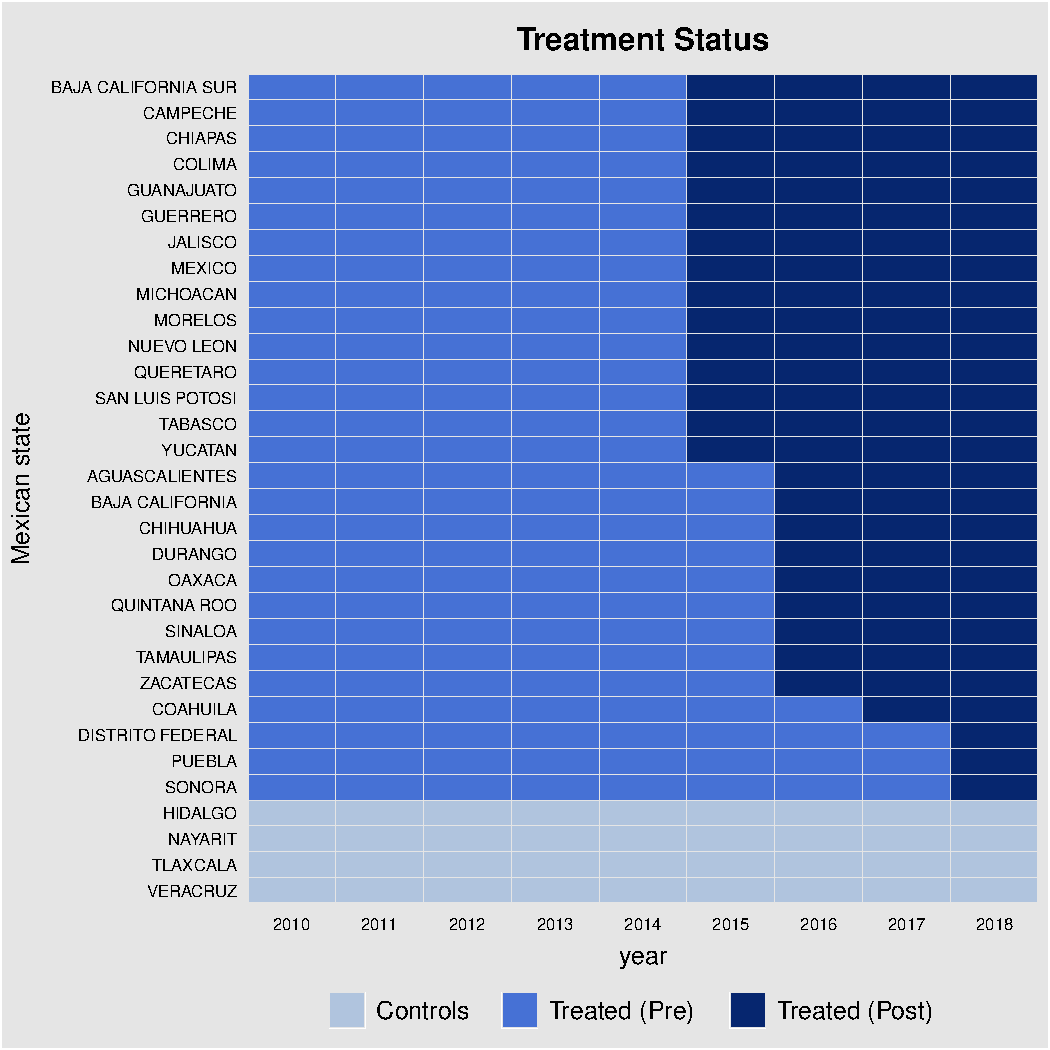
\includegraphics[width=0.75\textwidth]{Figures/reform_treatmentstatus.pdf}     
\captionsetup{justification=centering} 
\end{figure}   
 
    
A second source of discretion granted to state-level legislatures revolved around the reelection implementation date. The reform dictated that any change would not affect 2014 elections, and would be implemented for federal legislators till the elections of 2018. For local legislators and mayors, however, state-legislators defined the implementation period. Given governors influence in candidate selection of legislators (and mayors in some cases), their staggered calendar and political power seems to explain most of the variation in the timing of the implementation of the reform: governors with terms ending near the Reform approval date (2014) introduced reelection as early as possible, while those whose terms where starting pushed reelection further down the line. According to \citet{motolinia_2020}, governors ending their terms near 2014 had incentives to introduce reelection early on given that they could still apply political influence after leaving office by choosing people of their liking. Since governor influence is an important determinant of the timing of the implementation of the Electoral Reform, for causal identification is important to control for governors political power.\footnote{For more detail on the political background of the Electoral Reform see Appendix \ref{appendix:reform_backgorund}.}
   
Figure \ref{fig:treatment_status} describes the implementation period or treatment status of each of Mexico's 32 states.\footnote{Mexican states share the same administrative level as US states.} This figures allows to visualize the staggered rollout of the term limit removal. We have five timing groups. Four states never receive treatment during this time period (Hidalgo, Nayarit, Tlaxcala and Veracruz), while the rest commence treatment in different years from 2015 to 2019. %The always-treated group is composed by the states of Baja California Sur, Campeche, Chiapas, Colima, Guanajuato, Guerrero, Jalisco, Mexico, Michoacan, Morelos, Nuevo Leon, Queretaro, San Luis Potosi, Tabasco and Yucatan. 
Treatment in this Figure implies the following: Campeche, for example, begin treated starting in 2015 means that mayors elected in 2015 can run for reelection in the next election of 2018, as well as that of 2021 if they won in the previous one. Similarly, mayors in Chihuahua elected in 2016 can run for reelection in 2019, as well as 2022 since the reform allows mayors to reelect up to two consecutive terms.  

\section{Data \label{sec:data}}  

I use the Municipal Government Census (\emph{Censos de Gobierno Municipal}) in Mexico from 2011 to 2019 that registers whether the mayor signed a centralized command agreement with the governor in the previous year. I then construct a dummy indicator that takes the value of 1 if a mayor delegated the municipal security policy to the governor, and 0 otherwise. This indicator that runs from 2010 to 2018 is the main outcome in the paper. 

From 2014 onwards, the Municipal Census included additional questions of whether a mayor hold a security  cooperation agreement with other political actors besides the governor. It is important to note that these are \emph{cooperation} agreements, not \emph{delegation}agreements; in the former, mayors share responsible for public security provision, while in the latter they give the responsibility away to governors. There are several security cooperation agreements that mayors can sign in Mexico: (a) agreements between municipalities (e.g., to create metropolitan police forces), (b) between municipalities and the federal government, (c) agreements with multiplicity of executive actors (various municipalities, states, with or without the Federal government), and (d) agreements with other branches of government, including legislative and judicial ones, also at various levels of government. I construct a dummy of whether a municipality had a security cooperation agreement with other political actors besides the governor. This indicator serves as a falsification test of the theory on the incentive to differentiate from challengers in two ways. First, mayors up for reelection have no need to impress voters from other states and municipalities, so we would expect a null effect of reelection incentives on these cooperation agreements. Second, mayors do not share a security jurisdiction with federal police forces under the control of the president. The federal police does not dealt with local public security disturbances, and will only join municipal forces when crimes occur in federal areas such as airports or bus stations. As a result, there is no need to differentiate themselves from these security forces so null results from reelection incentives should be expected. We could believe that there is a need to differentiate municipal security effort from that of the military or marines, but these forces are quite distinctive already from local police authorities. As a result, mayors up for reelection should not have an incentive to differentiate themselves from these forces either. 

From the Municipal Census, I also construct dummy variables for the services delegated in centralized command agreements.  Mayors can delegate any of the following services to the governor: public security activities, traffic, security prevention, training, sharing of equipment and technology, research capacity, analysis and intelligence and the formation of unified criteria on procedures of public security institutions and laws. I also construct dummy variables for each of the reasons expressed to signing centralized command agreements with the governor, including a constitutional reform, change in local legislation, lack of resources, need of professionalization, a need for coordination, and given the prevalence of crime.
 

To proxy for citizens security preferences, I rely on the National Survey of Victimization from 2011 to 2019 (\emph{ENVIPE} in Spanish). ENVIPE collects state-level representative data on the year previous to the collection.  In particular, I focus on the question of the topic that worries citizens the most which include any of the following: narcotraffic, insecurity, the punishment of criminals, corruption, poverty, unemployment, health, inflation, natural disasters, water scarcity and education. I construct the average rate of responses by state-year. Four additional variables are constructed using the average response to the questions on the level of trust in police forces, whether citizens can identify them, their perceived level of corruption and efficiency.\footnote{The questions of trust and efficiency have a 4 item scale from ``a lot", ``somewhat", ``little", to  ``nothing" for either municipal, state or federal forces. I construct a dummy variable that takes the value of 1 for the items ``a lot" or ``somewhat" and 0 otherwise. The questions on whether citizens can identify each police force and corruption have only ``yes'' and ``no'' as response items. There are multiple police forces identified. I categorize them in the following way: traffic and preventive police forces correspond to the municipal level; state police and state attorney police forces to the state level; federal police, ministerial police, army and marines to the federal level.} 
 
Electoral data for recent Mexican elections at the governor and municipal level as well as data on the rollout of the electoral reform at the municipal level comes from \citet{magar_2012} and \citet{magar_2017}. The data compiled from multiple sources including state electoral institutes, Banamex Electoral Database, Voz y Voto, etc. contains voting counts per party. I construct winning margins at the municipal and state level as the difference between the first and second runner. Indicators to measure party-alignment between the federal executive, state and municipal governors are also build. The winning margin and party alignment with governors serve to control for governor's influence. 

Lastly, to test the effect of the Term Limit Reform on public security and violence, I build a database on violence and effort placed by federal and municipal-level security forces for all municipalities in Mexico from 2010 to 2018.\footnote{Mexico has 2,467 municipalities. Thus, the total possible number of observation is 22,203 municipality-years (2,467 municipalities X 9 years).} Violence is proxied by homicide related deaths collected by the National Institute of Statistics and Geography (INEGI for its acronym in Spanish).\footnote{INEGI reports two homicide datasets. One the one hand, homicide related deaths that come from the total death certificates marked as ``presumed homicides''. On the other hand, homicide statistics made up of the number of previous investigations initiated for the crime of homicide, by year and state. As noted by \citet{rivera_2012} these datasets do not coincide for a simple reason: the former counts bodies, the latter counts cases. I choose homicides based on death certificates since those based on initiated investigations tend to miscalculate the total number of deaths. For instance, borrowing a practical example by \citet{rivera_2012}, consider a mass grave with charred human remains. A preliminary investigation will count the number of deaths, and this will become part of the homicide related deaths figure. However, the investigation will only file one case, regardless of the number of victims found. I thus prefer to count victims rather than cases.} Population estimates come from the 2010 Census, the 2015 Population Count (both by INEGI), and CONAPO's population projections at the municipal level. Homicides per capita are highly skewed, with a long right tail of municipalities with substantially greater homicides than others. I therefore run the estimation on the impact of the reform on homicides per capita on logged values. For robustness, following \citet{mackinnon_maggie_1990}, I use the inverse hyperbolic sine (IHS) to transform the main outcome. %For robustness, I run estimates based on a second homicide database build by the SNSP.\footnote{For more detail on the SNSP homicide database please see Appendix \ref{appendix:SNSP_homicides}.}


To approximate the level of effort placed by municipal forces and the military, I build a novel database on narcotics, arms and laboratories eradicated by the military -army and marines- from 2006 to 2019 at the municipal level  based on information petitions through the Mexican portal INFOMEX.\footnote{Information petitions number 0000700274419 and 0000700274519.} The dataset includes narcotic eradication (kg) of marijuana, heroine, methamphetamine, and cocaine, as well as marijuana and poppy kg per hectare eradicated, destroyed laboratories, and secured cartridges, vehicles, planes, short and long weapons as well as the detection of clandestine airstrips.  Another information petition to INFOMEX was made for municipalities to report the number of criminal detentions made month by month to proxy local level police effort. Detentions were aggregated at the yearly and municipal level. As with homicides, detentions and narcotic eradication and laboratories detected are highly skewed. I transform detentions to per capita logged values (also IHS), and narcotic and laboratories using logged (IHS) values as well. A concern might be that these measures of effort are actually measures of violence or DTO activity. In all estimations, I use these measures of effort as outcomes conditioning regressions on the level of homicides. Presumably, conditional on the level of violence these variables will approximate the level of effort placed by security forces. As an additional level of effort,  I rely on INEGI's municipal level data on expenses from 2010 to 2018, including expenses in public security, social development and public infrastructure,  and wages to bureaucrats that include the salaries to local police forces. All expenses are deflated and in million pesos.\footnote{One dollar equates to roughly 20 pesos as of May of 2021. One million pesos is approximately \$50,000 dollars.} Lastly, to measure criminal presence, I rely on the 2010 cartel presence index from \citet{camilo_etal_2018}. 
 Appendix Table \ref{tab:descriptive} presents descriptive statistics of the variables used in the paper.
  
\section{Research Design \label{sec:design}}  
     
To investigate whether reelection incentives affected the delegation of security policy in Mexico, I explore the variation in the reelection incentives generated by the removal of term limits.  Specifically, I exploit the staggered implementation of the 2014 Electoral Reform in Mexico that removed term limits for mayors up to two periods. I compare first-term mayors who are term limited to first-term mayors who can be reelected. A first term mayor that can reelect and a first term mayor who is term-limited have won an election once, and thus have the same selection pressures but different electoral incentives. The difference between them yields the reelection incentive effect \citep{Besley_case_1995, ashworth_2012}. In other words, the research design allows to identify the reelection incentive and rule out the concern arising from selection, including differences in the experience and ability of incumbents \citep{ferraz_finan_2011}.\footnote{To estimate the selection effect, we could compare first term mayors (with or without term limits) who have won an election to second term mayors who have won an election once. The election incentives are the same but the selection is different \citep{ashworth_2012}.} 

A two-way fixed effect model (TWFE) at the municipal and year level would be the go to specification to test the effect of the Electoral Reform on the delegation of security policy by mayors. However, recent literature has shown that in the presence of staggered treatment timing and heterogeneous treatment effects across cohorts, the coefficient from TWFE models are not causally interpretable \citep{goodman_bacon_2018, callaway_santana_2019, strezhnev_2018, chaisemarting_etal_2019}. Furthermore, for event-study designs \citet{abraham_sun_2020} find that even under strong parallel trends assumption, pre-reform coefficients may not be non-zero and the post-reform coefficients may not correspond with a convex weighted averages of cohort-specific treatment effects at particular lags and leads. In other words, coefficients of a given lag or lead can be biased by the effects from other time periods, and pretrends may be driven by treatment effect heterogeneity. While I report the estimates from a TWFE model in the Robustness Section \ref{sec:robustness}, these results need to be interpreted with caution.
   
 To account for potential cohort treatment heterogeneity, I estimate  a cohort weighted event-study design following \citet{abraham_sun_2020} that exploits the staggered implementation of the reform and state-level variation. 
 I saturate the time and unit fixed effects structure so that treated units do not enter the test window as control units. Specifically, I replace the binary indicator variable for the start of the treatment reform with a series of lead/lag indicators $\gamma_k$ for being ``k" years away from treatment. I focus on the window from 8 years prior to treatment to three years afterwards i.e. for $k \in \{-8,3\} $ which correspond to the time period of 2010 to 2018, with 2015 the first year of Term Limit Reform implementation.\footnote{See Figure \ref{fig:treatment_status} where those treated in 2018 have 8 lags prior to treatment, while those treated in 2015 have 3 leads, the full window of analysis for $k \in \{-8,3\} $.} %In addition to including $\gamma_k$ for $k \in \{-8,3\} $, I saturate the model with indicators for years less than 3 years before treatment, and more than three years after treatment. 
I exclude the indicator on $\gamma_{-1}$ to avoid collinearity and for comparison: estimated coefficients are interpreted as the difference relative to $t-1$, i.e. one year prior to the implementation of the electoral reform. Following   \citet{abraham_sun_2020}, I also exclude $k=-8$ due to collinearity. The estimated equation is as follows:


 
 \begin{equation}
\label{eq:abraham} 
y_{mt}=\mu_m + \mu_t + \sum^{5}_{e=1} \sum^3_{k=-7, \neq {-8,-1}} \gamma_{e,k}(1\{E_i=e\} \cdot R^k_{m,t}) + \sum^{5}_{e=1} \sum^3_{k=-7, \neq {-8,-1}}  \Theta'X_{s(m)t} (1\{E_i=e\} \cdot R^k_{m,t}) + \epsilon_{mt}
%y_{mt}=\mu_m + \mu_t + \sum^5_{e=1} \sum^{3}_{k \neq {-8,-1}} \gamma_{e,k}(1\{E_i=e\} \cdot R^k_{m,t}) + \sum^5_{e=1} \sum^{3}_{k \neq {-8,-1}}  \Theta'X_{m(s)t} (1\{E_i=e\} \cdot R^k_{m,t}) + \epsilon_{mt}
%y_{mt}=\mu_m + \mu_t + \sum^5_{e=1} \sum^{3}_{k \neq {-1,-8}} \gamma_{e,k}(1\{E_i=e\} \mathbbm{1} (t-I_{m}=k)  ) + \sum\limits^{3}_{k=-8, k \neq -1} \Theta'X_{it} \mathbbm{1}(t-I_{m}=k) + \epsilon_{mt}
%y_{mt}=\mu_i + \mu_t + \sum^5_{e=1} \sum^{3}_{k \neq {-1,-8}} \gamma_{e,k}(1\{E_i=e\}\cdot R^k_{m,t} ) + \sum\limits^{3}_{k=-8, k \neq -1} \Theta'X_{it} \mathbbm{1}(t-I_{m}=k) + \epsilon_{mt}
\end{equation} 
  
where $y_{mt}$ is a dummy that takes the value of 1 if the mayor signed a centralized command agreement with the governor, 0 otherwise. $E_i$ are cohort-specific indicators if a Mexican state removed term limits in a given year.\footnote{As noted in Figure \ref{fig:treatment_status}, there are five treatment cohorts including the never treated. The never-treated cohort is made up of the municipalities in the states of Hidalgo, Nayarit, Tlaxcala and Veracruz.} $R^k_{m,t}\in \{0,1\}$  is the Term Limit Reform treatment status indicator at period $k$ relative to treatment, for municipality $m$ at calendar time $t$.\footnote{$t=e+k$.} $\mu_m$ and $\mu_t$ are the municipal and time fixed effects. $X_{s(m)t}$ is a matrix of state $s$ (municipal $m$) level covariates interacted with the set of cohort-specific fixed effects including pre-treatment governor's winning margin, party alignment with the governor, party alignment with the President, mayor's winning margin, logged homicide related deaths per capita, and a dummy indicator on the presence of cartels.  The year indicators by treatment cohort  $\gamma_{e,k}$ are the difference-in-difference (DiD) estimators for the Cohort Average Treatment Effects (CATTs). Conditional on municipal and period fixed effects, as well state-level covariates, these CATTs represent the annual difference in mean centralized command agreements signed with governors between municipalities that removed term-limits relative to those that did not, $k$ years before and after treatment. Standard errors are clustered at the state-level as that is the treatment level of the Term Limit Reform. Since the number of clusters is small (32 states), I adjust standard errors using wild bootstrap when indicated. 

I take the linear combination of the CATTs for each relative time period $k$, weighting each cohort by its relative share of the sample, to construct the interaction weighted (IW) estimator of \citet{abraham_sun_2020}:   

\begin{equation}
\hat{\nu}_g=\frac{1}{|g|}\sum_{k \in g}\sum_e \hat{\gamma_{e,k}} \hat{Pr}\{E_i=e | E_i \in [-k, T-k]\}	
\end{equation}

where $\hat{\gamma_{e,k}}$ is returned from equation \ref{eq:abraham} and $\hat{Pr}\{E_i=e | E_i \in [-k, T-k]\}$  are the estimated weights equal to the share of each cohort in the relevant time period, normalized by the size of  $g$, with $g$ the universe of the $k$ periods relative to treatment. Since I estimate a IW estimator per year $|g|=1$. Lastly, to estimate the average treatment effect from $t$ to $t+3$ I run the linear average of weighted coefficients across the CATTs of those time periods relative to treatment. 

\section{Main Results \label{sec:results}}


   
Figure \ref{fig:event_study_agreements} reports the IW estimator %\footnote{From here on all tables report IW estimators.} 
 for each lead and lag relative to the first year a municipality implemented reelection. In average from $t$ to $t+3$ , reelection incentives decreased the likelihood of signing centralized command agreements by 41.97\% significant to the 5\% level. In magnitude, this result represents 1.5 times the mean or almost 1 standard deviation. In other words, compared to term limit incumbents, incumbents seeking reelection will decrease the delegation of security policy to the governor. This is true whether we adjust the standard errors for the small number of clusters using wild bootstrap or not (see Appendix Table \ref{tab:as_agreements}).\footnote{Including a lag outcome may introduce Nickell bias. More importantly, the lagged outcome conflates controls for heterogeneity and modeling dynamic treatment effects. To avoid these problems I only control for pretreatment outcomes to deal with heterogeneity and do not include  any lags of the dependent variable. Alternatively, I use matching on pre-treatment outcomes and find that results show similar effects (see Section \ref{sec:robustness}).}   
         
     
If delegation of security policy decreases, what specific services are provided by incumbents? Figure \ref{fig:services} shows that incumbents with reelection incentives decrease signing agreements that delegate the service of public security (-10.31\% significant to the 1\% level) and also public traffic (2.4\% significant to the 5\% level). Meanwhile, those related to capacity building are not different relative to term-limited mayors including training, equipment and technology, research and intelligence and the unification of laws and procedures. These differences may come from incumbents up for reelection caring only about services that are more visible to constituents or that they care more about, mainly public security and traffic; all other services form part of the back office of public security provision.  

\begin{figure}[h] 
\centering
 \caption{Effect of Term Limit Reform on Security Cooperation Agreements signed with the Governor, 2010-2018}
 \label{fig:event_study_agreements}
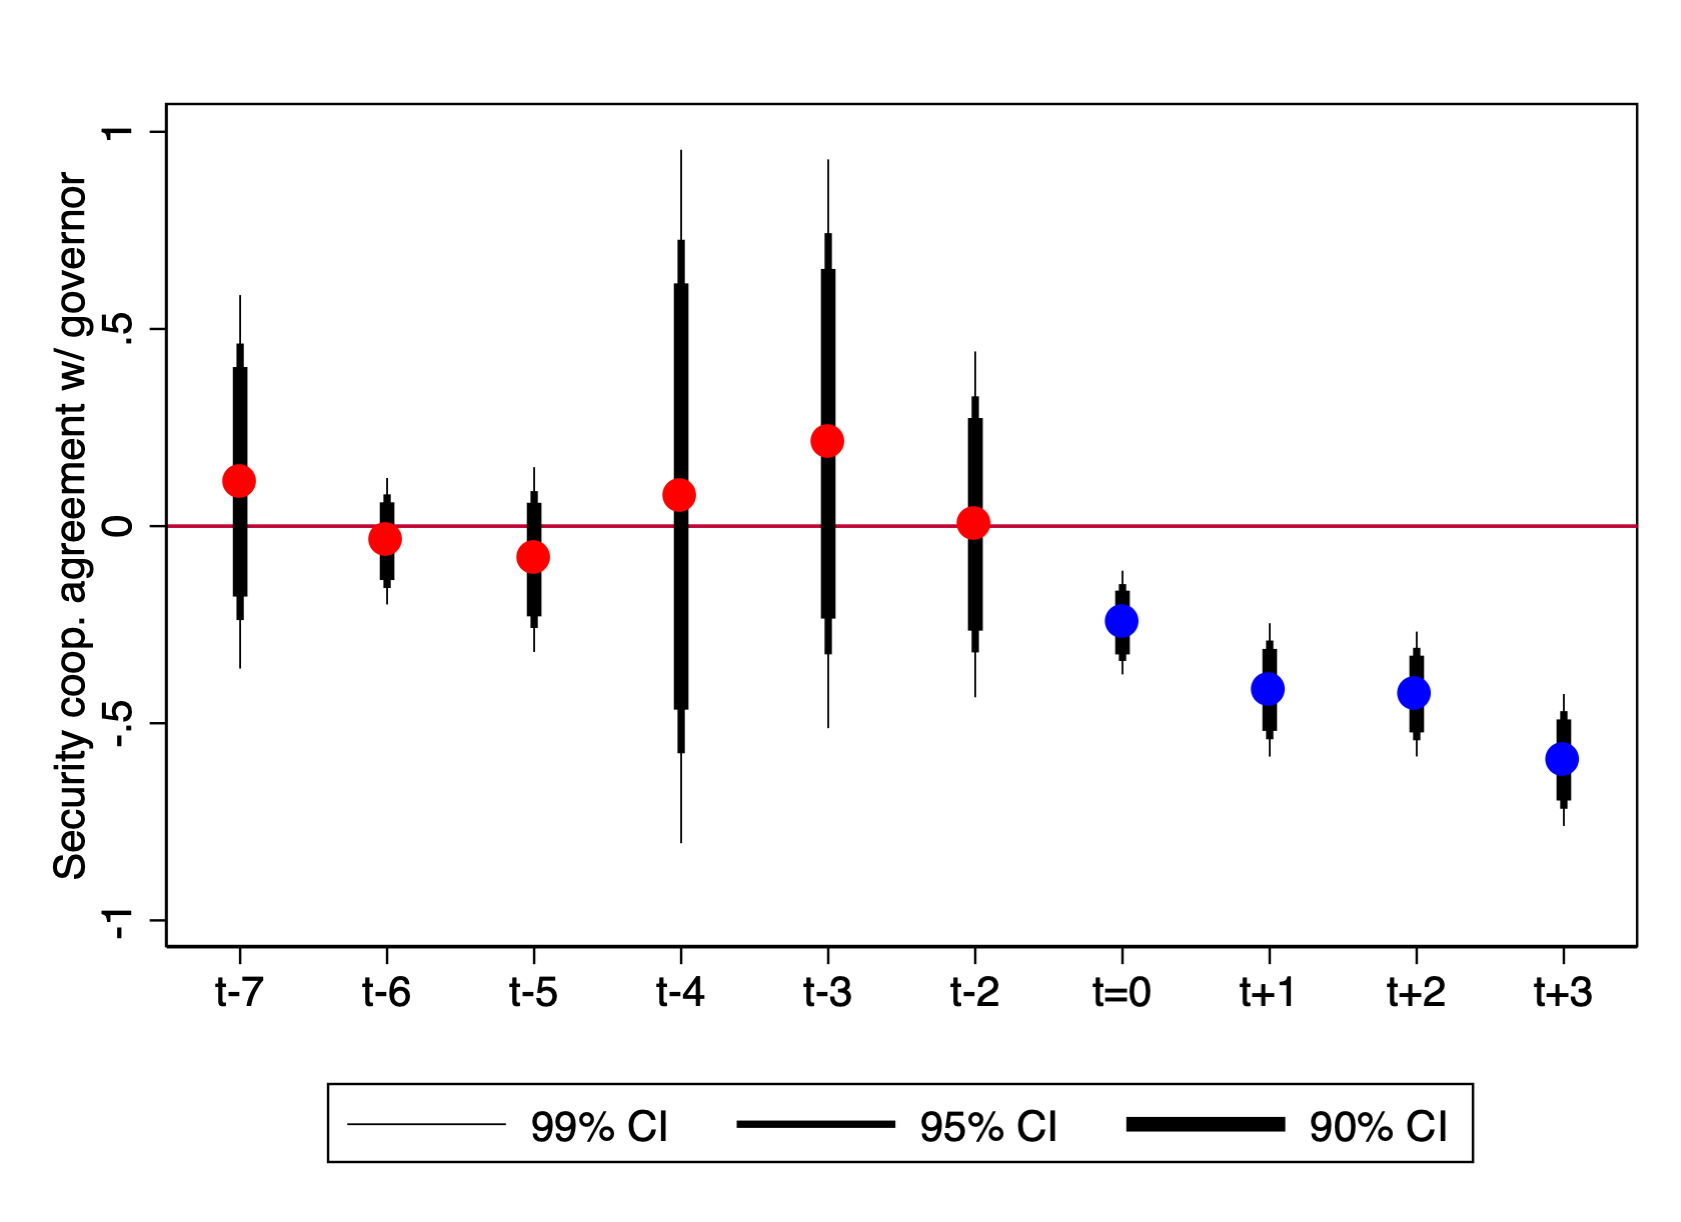
\includegraphics[width=0.75\textwidth]{Figures/catts_agreements.png}
       \captionsetup{justification=centering}
       
 \textbf{Note:} Figure \ref{fig:event_study_agreements} shows the IW estimators following \citet{abraham_sun_2020} for each lead and lag relative to the first year a municipality implemented reelection. Red points are pre-treatment, while blue ones post-treatment. 
     
\end{figure}   

 \begin{figure}[h]   
\centering
 \caption{Comparison: Security Cooperation Agreements with Governor vs. Other Actors, 2014-2018}
 \label{fig:services}
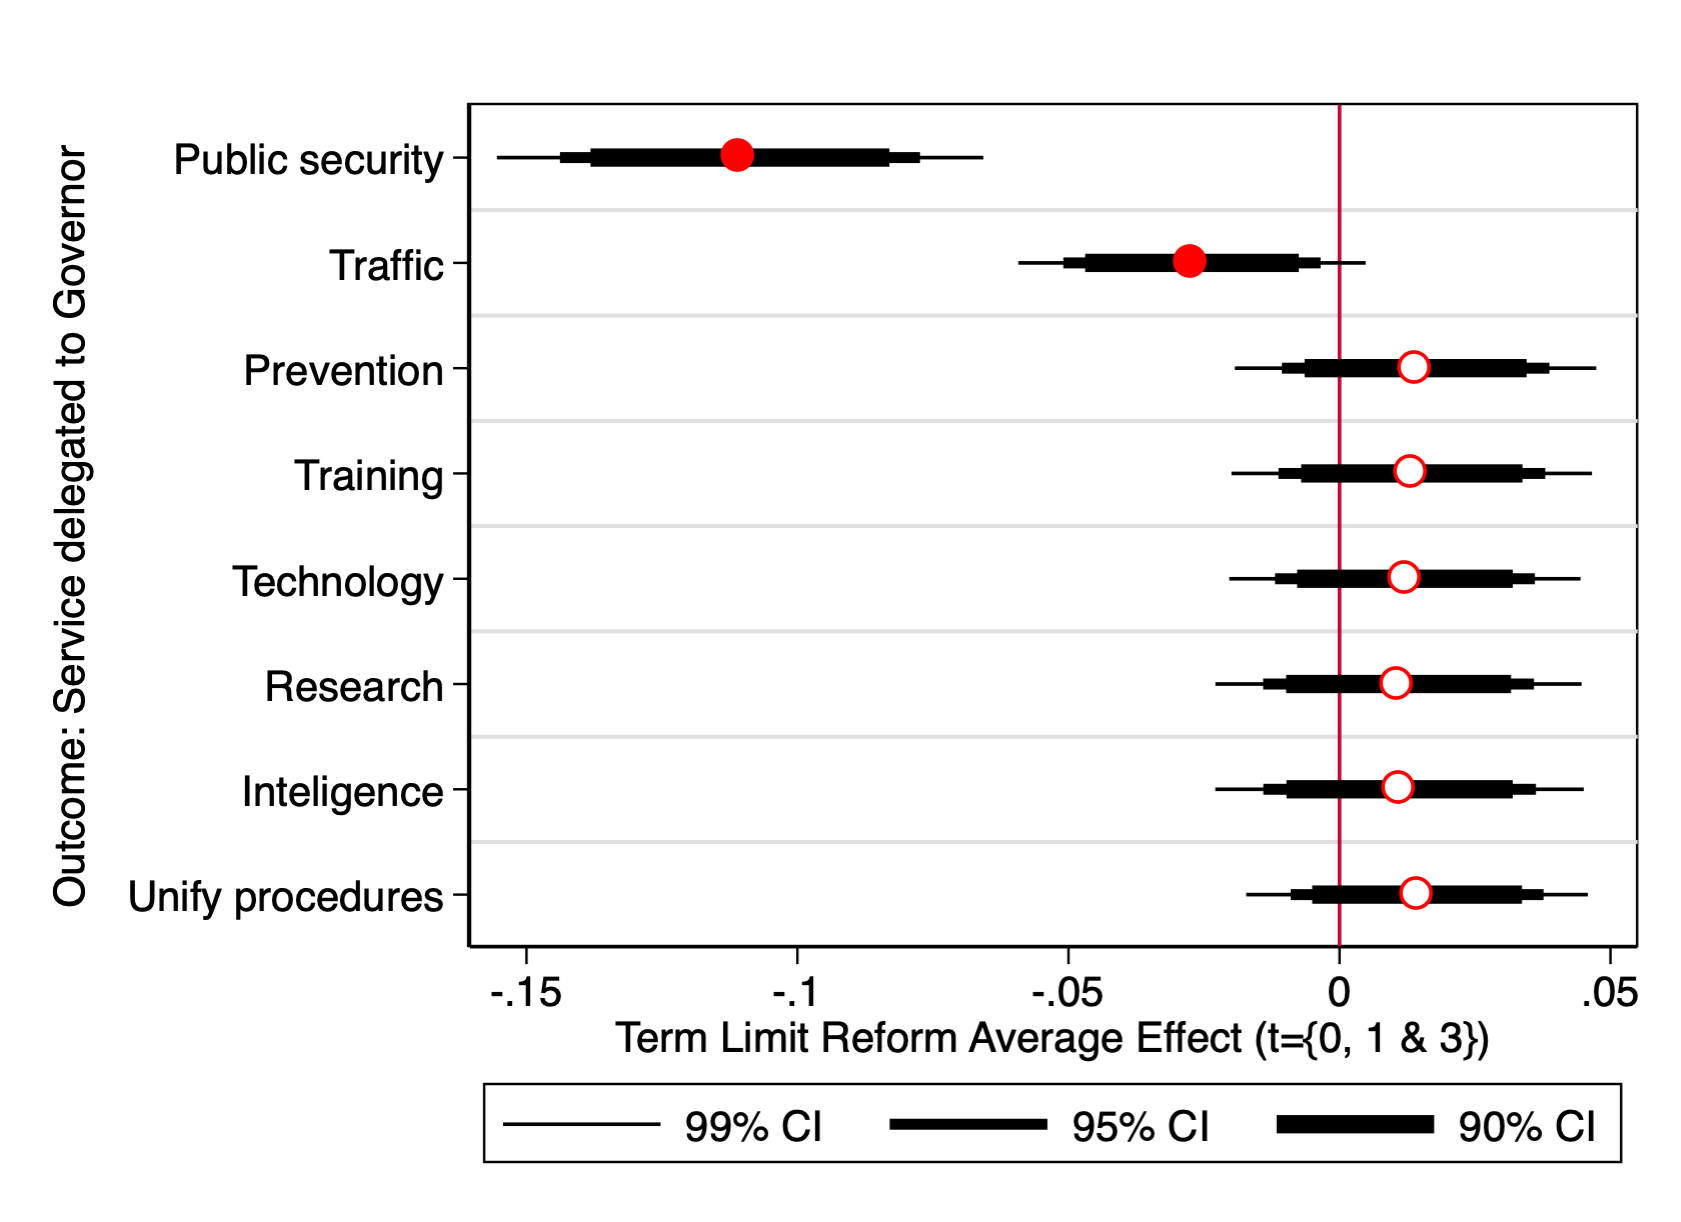
\includegraphics[width=0.65\textwidth]{Figures/services.png}
       \captionsetup{justification=centering}
       
 \textbf{Note:} Figure \ref{fig:services} shows the average treatment effect from t, t+1 and t+3 across multiple specifications. This average effect was estimated using the IW estimators following \citet{abraham_sun_2020} for each lead and lag relative to the first year a municipality implemented reelection. Red points show that parallel trends hold, while hollow ones imply pretrends. 
\end{figure}  

\subsection{Identification \label{sec:identification}}
 
Once we consider cohort weights, I find strong evidence of parallel trends as noted in Figure \ref{fig:event_study_agreements}.\footnote{Without cohort weights, the naive event-study design shows pretrends. However, these estimates are biased due to potential treatment effect heterogeneity across treatment cohorts.} Besides no pretrends, identification in this setting implies that the staggered roll-out of the Term Limit Reform is orthogonal to municipal-specific characteristics, conditional on municipal and year fixed effects. This implies {\emph as-if} random assignment to the treatment status visualized in Figure \ref{fig:treatment_status}. If say, strong governors delay or adjust the implementation of the reform according to their political agenda, then identification would fail. To address this problem equation \ref{eq:abraham} interacts the state covariates with cohort-specific fixed effects to adjust for any changes correlated to the evolution of governors strength, the term $X_{s(m)t} (1\{E_i=e\} \cdot R^k_{m,t})$. Pretreatment covariates include governor winning margin and an indicator of governor party alignment with the president, since pressure from former President Enrique Peña Nieto modified state legislators approval of the electoral reform, particularly for PRI states (for more detail see Appendix Section \ref{appendix:reform_backgorund}). Identification assumption implies now that conditional on municipal and year fixed effects, and cohort specific linear trends in state-level covariates, unobserved factors are not correlated with the electoral reform treatment assignment over time. I further validate this by following \citet{altonji_etal_2005} to check if unobserved variation is likely to explain the signing of centralized command agreements with the governor by mayors. I regress the treatment (whether the municipality held reelection) on all the available covariates used for Figure \ref{fig:event_study_agreements}. I then take the fitted value from the regression and use it to predict each outcome, this time including unit and year fixed effects. Appendix Table \ref{tab:unobservables} suggests that – under the assumption that observables are representative of unobservables – selection on unobservables is not driving the results. 

An additional identification assumption in event-study designs speaks to no anticipatory behavior from municipalities to the Term Limit Reform. If states or municipalities had private knowledge of the future treatment path this may change their behavior in anticipation to being treated and thus the potential outcome prior to treatment may not be that of baseline outcomes: estimated coefficients may reflect the anticipatory effects of the reform rather than differences in untreated potential outcomes between untreated and treated groups. %\citep{malani_rief_2015}.
%In this setting, knowledge from incumbents of the term limit removal could lead to a decrease in public security (and public good) provision since this will be the period a term limited politician could extract rents or pursue clientelistic practices without the electoral penalty of reelection. The violation of this identification assumption would lead to a (positive) bias of concern. 
I test this assumption by comparing if early and late adopters differed in their estimated effects. As seen in Appendix Figure \ref{fig:CDLZ_agreements}, this is not the case: there is wide variation in estimated coefficients across early (red) and late (blue) adopters of the reform.\footnote{For more detail on how I compare early to late adopters, please see Appendix \ref{appendix:CDLZ}.}  

In short, taking together parallel trends, evidence on no-anticipatory behavior from municipalities (and states) and cohort weighted estimates that account for treatment effect heterogeneity, I find a robust and unbiased negative effect of reelection incentives on the delegation of security policy from mayors to governors in Mexico.  The following sections further probe the results through different robustness and falsification tests.
         

\subsection{Robustness Tests and Secondary Research Designs \label{sec:robustness}}
 
  Figure \ref{fig:robustness_agreements} compares 6 models (see also Appendix Table \ref{tab:as_aggregate}). I find the naive two-way fixed effect model by municipality and year to reflect a negative non-significant effect of reelection incentives on delegation. However, pretrends are found and results need to be interpreted with caution as non-weighted estimates are biased \citep{abraham_sun_2020} as discussed in Section \ref{sec:design}. Adjusting standard errors using Wild bootstrap yields similar results for the naive two way fixed effect model. However, the main cohort weighted event study design with and without standard error adjustment using Wild bootstrap shows parallel trends and significant results. This result holds when changing the reference period from $t-1$ to $t=0$. Results also hold when performing the common practice of trimming relative time periods relative to treatment \citep{borusyak_2017, dobkin_etal_2018}, in this case by trimming all periods prior to $t-4$ to be balanced in relative periods. Moreover, across specifications the average effect from $t$ to $t+3$ remains relatively similar. 
        
  
\begin{figure}[h]   
\centering
 \caption{Effect of Term Limit Reform on Security Cooperation Agreements signed with the Governor, 2010-2018}
 \label{fig:robustness_agreements}
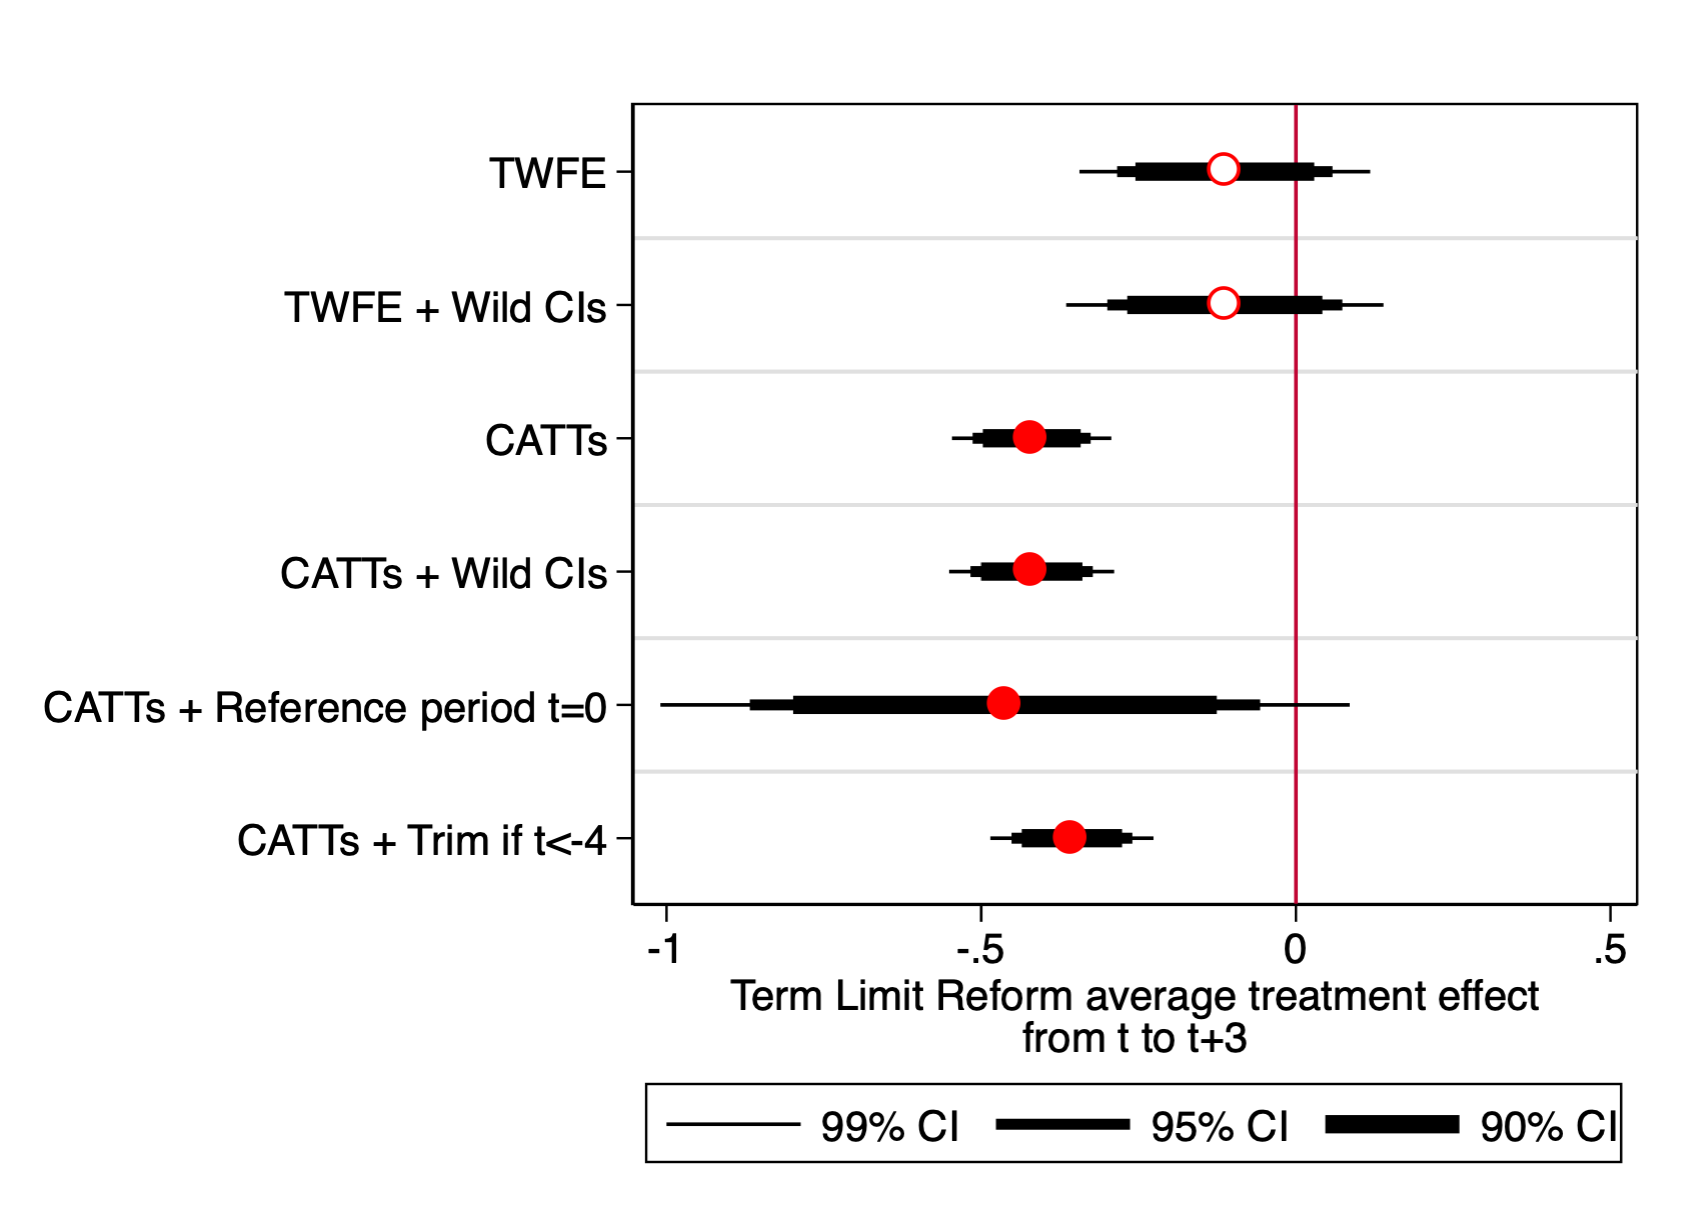
\includegraphics[width=0.75\textwidth]{Figures/average_effects.png}
       \captionsetup{justification=centering}
       
 \textbf{Note:} Figure \ref{fig:robustness_agreements} shows the average treatment effect from t to t+3 across multiple specifications. This average effect was estimated using the IW estimators following \citet{abraham_sun_2020} for each lead and lag relative to the first year a municipality implemented reelection. Red points show that parallel trends hold, while hollow ones imply pretrends. 
\end{figure}   

Further validation is provided by the use of secondary research designs including \citet{imai_etal_2020} non-parametric generalization of the difference-in-difference estimator that does not rely on linearity assumption and corrects for invalid negative weighting in standard two-way fixed effects models (see Appendix Figure \ref{fig:matching}), as well as \citet{chaisemarting_etal_2019} difference-in-difference with multiple time period correction (see Appendix Figure \ref{fig:chaisemarting_agreements}). In both cases we observe that reelection incentives led to a decrease in the signing of centralized command agreements, i.e. a decrease in delegation of security policy to the governor.

\section{Evidence on the Differentiation Mechanism\label{sec:heterogeneous}}

As discussed in Section \ref{sec:reelection_incentives}, we would expect incumbents with reelection incentives to send credit claim messages to portray competence or a strong type and difference themselves from challengers and the governor. They can do so by taking charge of security policy instead of delegating it to the governor. If this is true, we would expect this behavior to be more salient when  (i) citizens are concerned about violence, and (ii) when citizens are capable of rewarding or punishing mayors for security policy. 

\subsection{Heterogeneous Treatment Effects by Citizens' concerns}

In the context of American politics, for example, \citet{list_sturm_2006} find that governors seeking reelection adopt greener policies when their states hold large pro-environmental groups, while the opposite occurs in those with lower environmental support. In a similar tenor, we would expect that when a large proportion of citizens hold security concerns as the most worrisome topic then incumbents with reelection incentives will choose not to delegate security policy to the governor.   

This is what we find in Figure \ref{fig:preferences_all} Panel A that shows an interaction between the treatment of the Electoral Reform on narcotraffic as the topic that citizens´ worry the most. The baseline reform effect is statistically indistinguishable from zero. However, when a large proportion of citizens see narcotraffic as the topic they worry the most, mayors with reelection incentives decrease the delegation of security policy to governors relative to term-limit mayors. It is important to note that this finding is conditional on    pre-treatment violence levels, i.e. the differences in the concern of narcotraffic or delegation are not explained by differences in levels of violence but variation in idiosyncrasies between Mexican states.

 The same result is not find with insecurity or punishment to criminals as the topics that citizens worry the most. For insecurity we don't find parallel trends prior to treatment, and for punishment to criminals the result is not distinguishable from zero. More data on citizens security preferences would be needed to further validate the heterogeneous treatment effects found in Panel A. 
 
 However, to provide further validity Figure \ref{fig:preferences_all} Panels D to L run a placebo test:  they include other topics that citizens worry the most but are not related with public security provision. Since these topics are not related to security policy we should expect a null result. This is what we find and, in some cases, even positive interaction effects. These positive cases belong to topics that are of the national order in which cooperation with upper level governments is needed such as natural disasters and water scarcity. Interestingly, in these two cases the state and federal security forces, specially the military, have a very important role to solve the problem. 
 
\begin{figure}[h]   
\centering
 \caption{Electoral Reform Interaction Effects by Topic that Worries Most to Citizens}
 \label{fig:preferences_all}
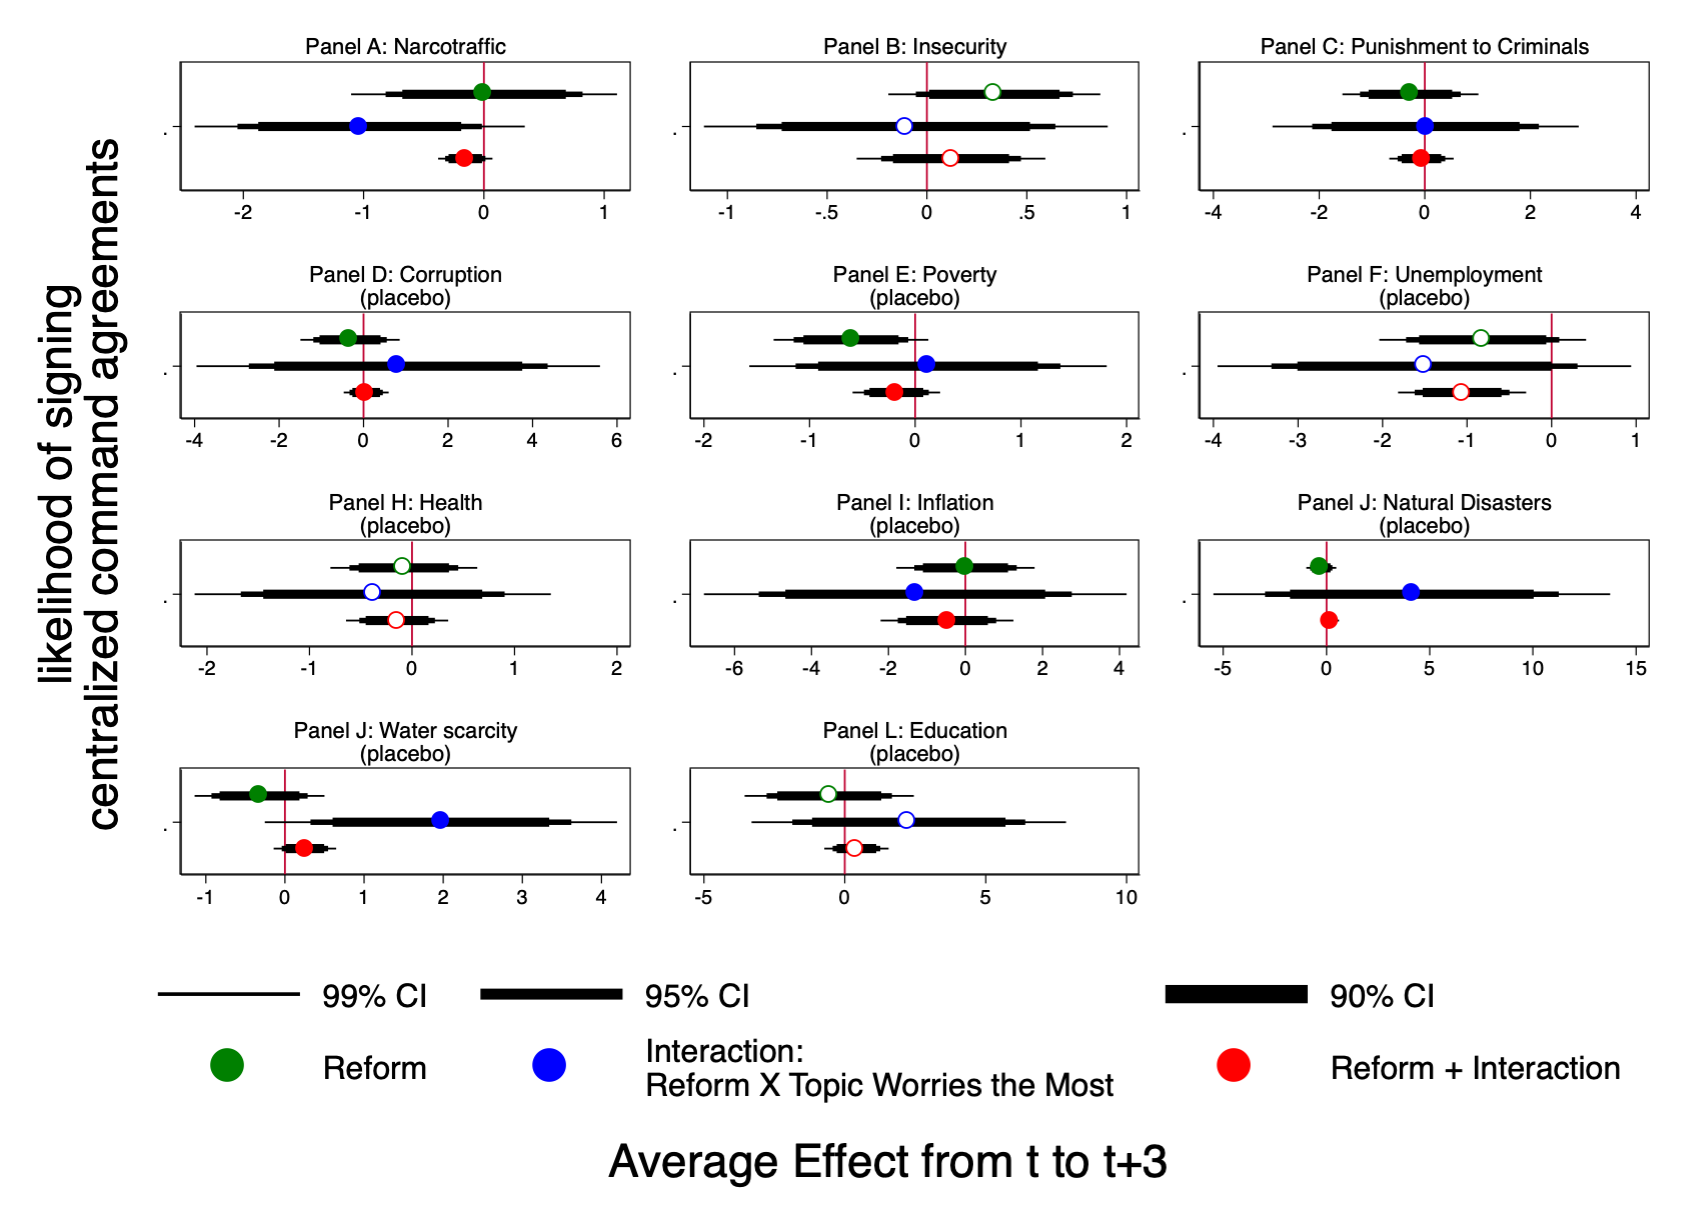
\includegraphics[width=1\textwidth]{Figures/preferences.png}
       \captionsetup{justification=centering}
        
 \textbf{Note:} Figure \ref{fig:preferences_all} shows the estimates of interacting the 2014 Term Limit Reform on the proportion of citizens that state that the topic stated worries them the most. This beliefs are pre-treatment. Point estimates show the average treatment effect from t to t+3. This average effect was estimated using the IW estimators following \citet{abraham_sun_2020} for each lead and lag relative to the first year a municipality implemented reelection. Filled points show that parallel trends hold, while hollow ones imply pretrends.  
\end{figure}    


\subsection{Heterogeneous Treatment Effects by Citizens Capacity to Determine Mayors as Responsible for Security Policy}
  
For incumbents with reelection incentives to care to impress voters, citizens need to be able to blame and reward incumbents for local security policy. In the case of Mexico, \citet{ley_2017} shows that citizens hold the capacity to blame (and reward) mayors for security policy if their party is aligned with that of the governor. Therefore, if there is alignment with the governor, we should expect mayors to decrease the delegation of security policy to differentiate themselves. In contrast, with alignment with other political actors like the president, citizens cannot clearly identify the responsible decreasing the incentive mayors have to differentiate themselves from other political actors by taking charge of security policy. In this case null results should be expected. Consider this a placebo test.
  
Figure \ref{fig:alignment} shows the interaction effect of party alignment on the Term Limit Reform. As expected in the interaction of Panel A, when there is alignment with the governor mayors up for reelection decrease the delegation of security policy to the governor, a result significant to the 5\% level. However, when not aligned as showed by the reform baseline result the coefficient is not different from zero. 

In contrast, in Panel B on the alignment with the president we find null results (and slightly positive) as expected, since citizens cannot assign responsibility to mayors for public security provision. 

\begin{figure}[h]   
\centering
 \caption{Reform interaction with Party Alignment}
 \label{fig:alignment}
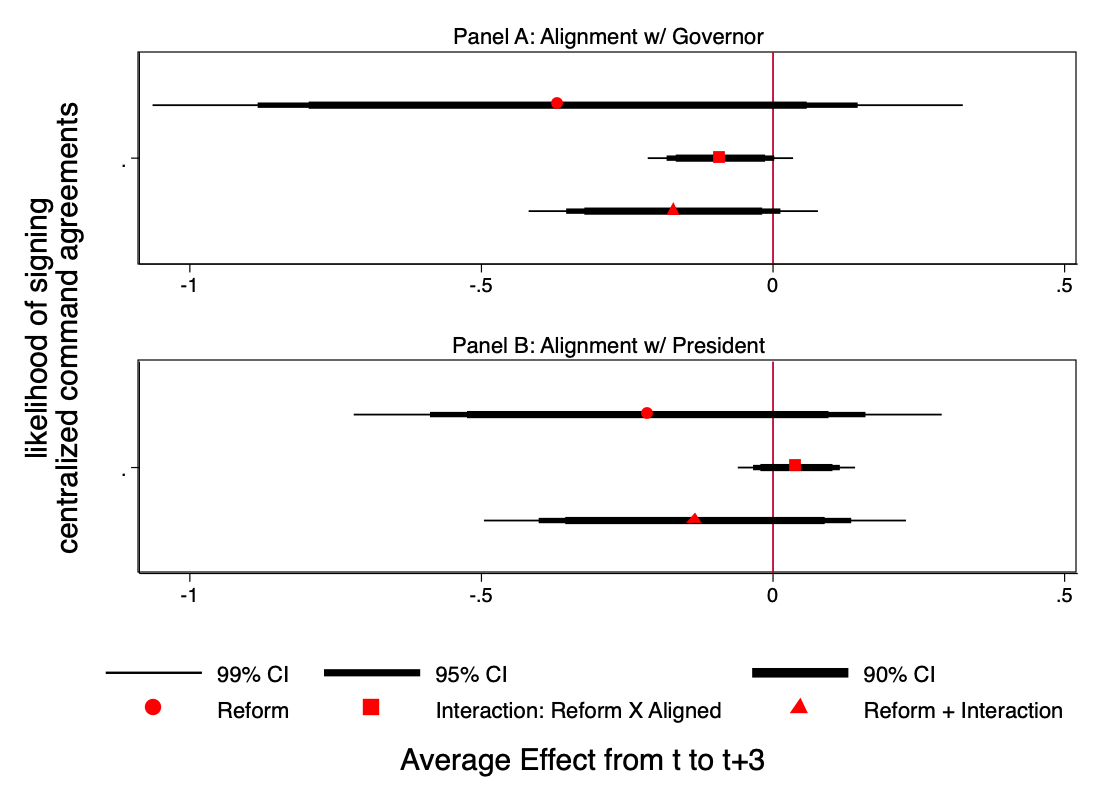
\includegraphics[width=0.9\textwidth]{Figures/interaction_alignment_full.png}
       \captionsetup{justification=centering}
       
 \textbf{Note:} Figure \ref{fig:alignment} shows the average treatment effect from t to t+3 across multiple specifications. This average effect was estimated using the IW estimators following \citet{abraham_sun_2020} for each lead and lag relative to the first year a municipality implemented reelection. Red points show that parallel trends hold, while hollow ones imply pretrends. To check parallel trends see Appendix Figure \ref{tab:interaction_alignment}.  
\end{figure}  
	
\subsection{Further validity on the differentiation mechanism: A Placebo Test on Security Agreements with Other Political Actors}


Now, I run a placebo test by seeing the effect of the reform on security cooperation agreements signed with the president, governors from other states and other municipalities. As described in the Data Section \ref{sec:data}, this security cooperation agreements serve as placebos as mayors do not hold an interest to differentiate themselves from these actors,  since the president's federal security forces do not deal with local public security, and governors and mayors from other states and municipalities are no electoral challengers. As expected, the falsification test in Figure \ref{fig:comparison_fed_estatal} shows a positive and non-significant effect for signing security cooperation agreements with other actors besides the governor. Meanwhile, similar to centralized command agreements, for security cooperation agreements with the governor in which the mayor continues to exercise responsibility in public security policy (i.e. these agreements do not imply delegation) we see a negative and significant effect. Mayors up for reelection choose to decrease not only the delegation of public security but also the reliance of any other type of cooperation agreements with the governor to whom they wish to differentiate themselves, and to differentiate from challengers as well.    
  
 \begin{figure}[h]   
\centering
 \caption{Comparison: Security Cooperation Agreements with Governor vs. Other Actors, 2014-2018 \\ -outcome: signing security cooperation agreement-}
 \label{fig:comparison_fed_estatal}
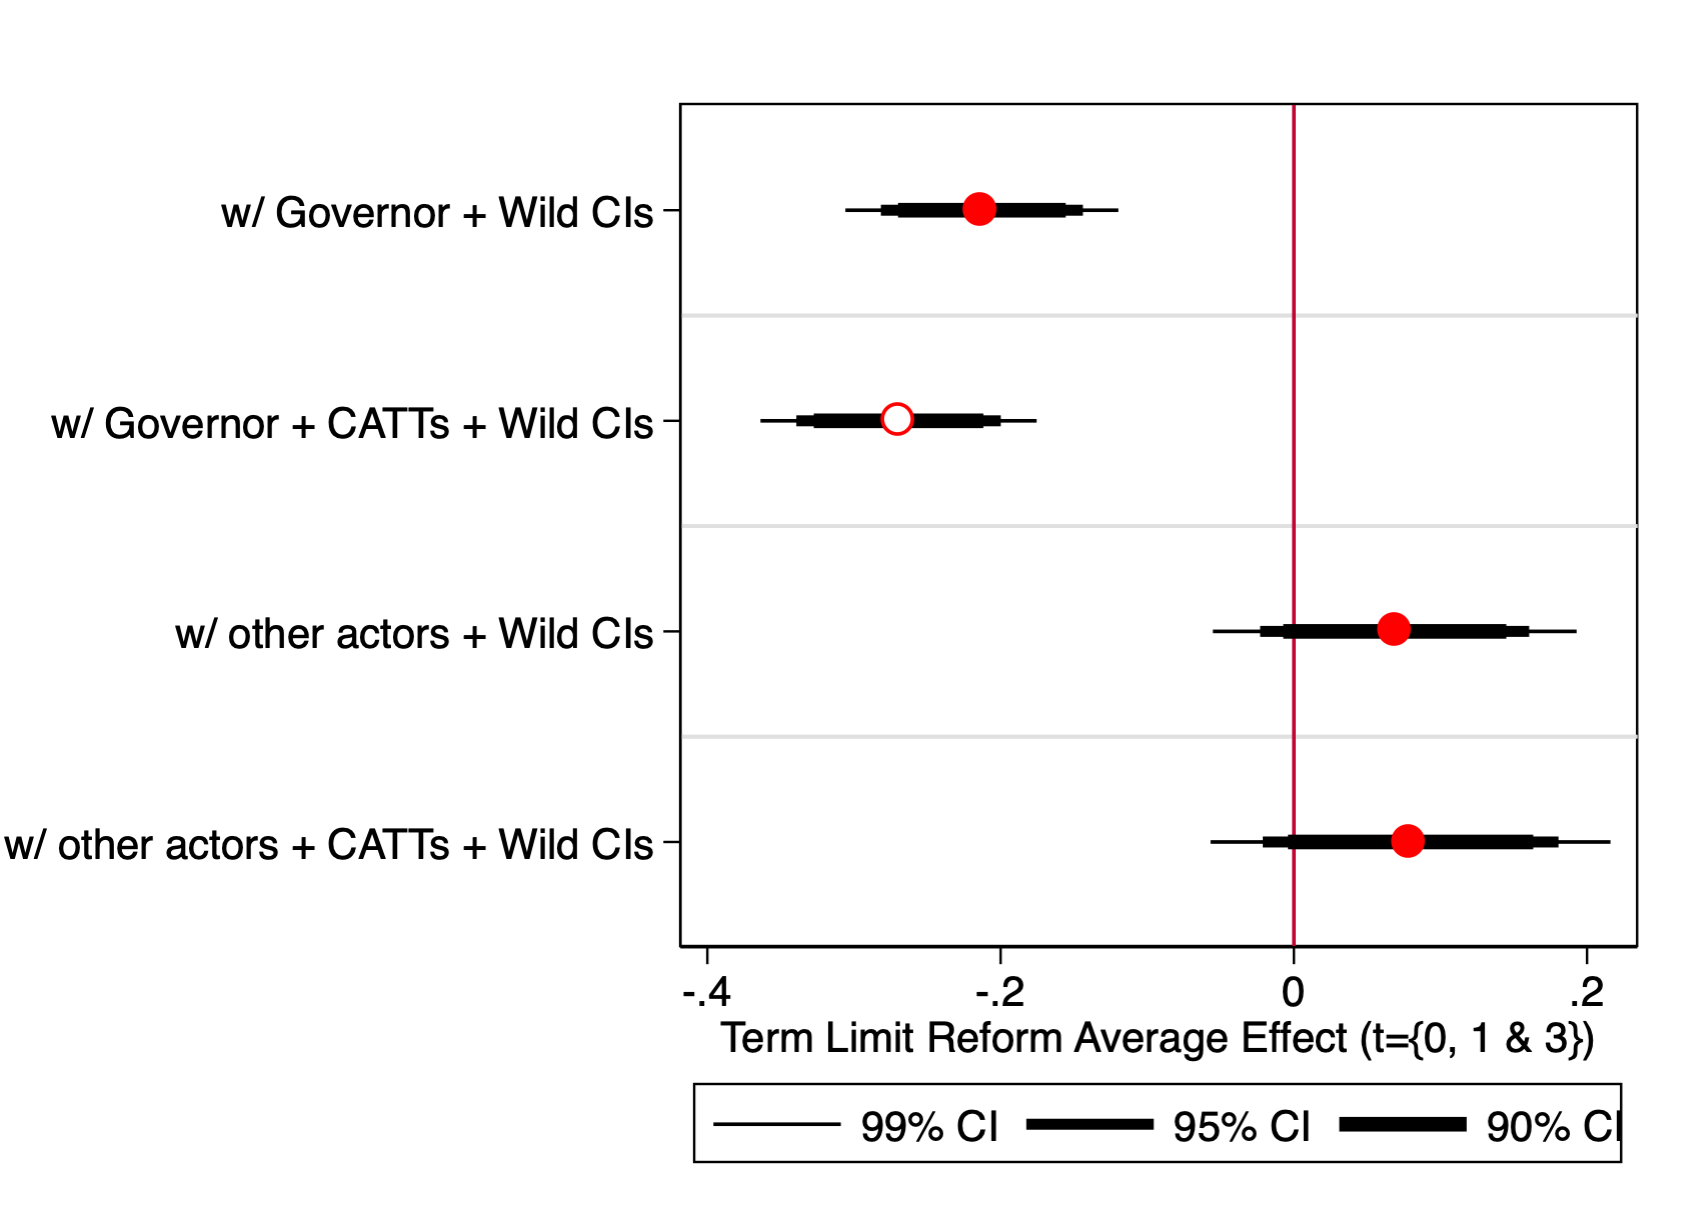
\includegraphics[width=0.75\textwidth]{Figures/average_effects_comparisonfedest.png}
       \captionsetup{justification=centering}
       
 \textbf{Note:} Figure \ref{fig:comparison_fed_estatal} shows the average treatment effect from t to t+3 across multiple specifications. This average effect was estimated using the IW estimators following \citet{abraham_sun_2020} for each lead and lag relative to the first year a municipality implemented reelection. Red points show that parallel trends hold, while hollow ones imply pretrends. 
\end{figure}   

\subsection{Credit Claiming or Responsiveness?}

As discussed in Section \ref{sec:reelection_incentives}, it is important to differentiate between credit claiming and responsiveness, i.e. between an exercise to send a signal to voters or actually addressing voters concerns. The difference is not minimal, as the latter implies the strengthening of accountability while the former does not. A way to empirically disentangle these two mechanisms is to assess the level of effort placed by mayors to tackle organized crime. 

Figure \ref{fig:effort} shows that while the effort placed by the local police in municipalities with mayors seeking reelection remains similar to that of term-limited incumbents as measured by the number of detentions per capita made by the municipal police, we observe a decrease in anti-narcotic activities by federal and state-level forces. Since we condition for pre-treatment levels of violence, we could consider these measures as proxies for effort. Therefore, there is no difference in the level of effort placed by mayors up for reelection to those that are term-limited which could be an evidence of credit claiming rather than responsiveness. Moreover, results show that the effort of federal forces does decrease leaving mayors to their luck to fight crime.

\begin{figure}[h]  
\centering
\caption{Effect of Term Limit Reform on Effort of Local and Federal Security Forces} 
\label{fig:effort}

   
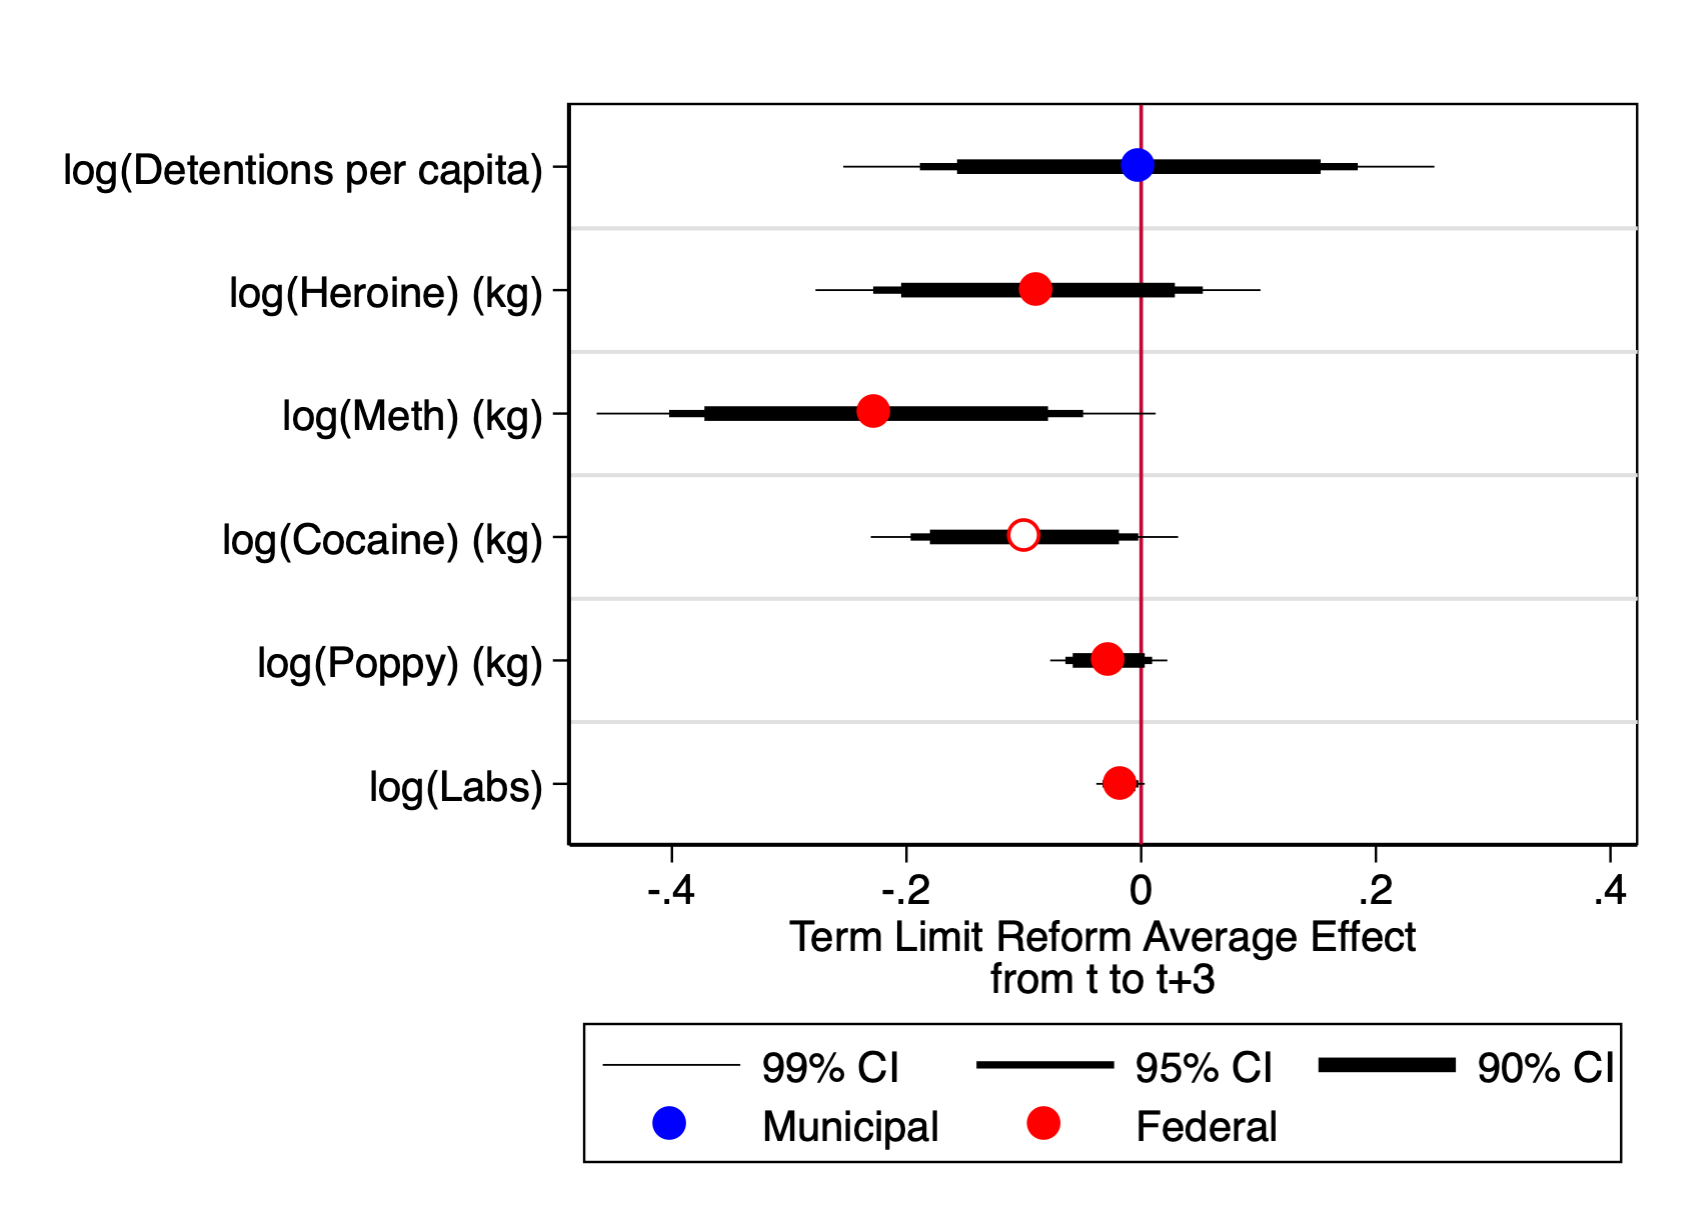
\includegraphics[width=0.75\textwidth]{Figures/effort.png}
  
 \textbf{Note:} Figure \ref{fig:effort} shows the average treatment effect from t to t+3 across multiple specifications. This average effect was estimated using the IW estimators following \citet{abraham_sun_2020} for each lead and lag relative to the first year a municipality implemented reelection. Filled points show that parallel trends hold, while hollow ones imply pretrends.        
\end{figure} 

If there are concerns that anti-narcotic measures or local police force detentions proxy for violence and not effort, we can rely on another measure of effort placed by mayors in office: expenses in public security. Figure \ref{fig:expenses} shows mayors up for reelection decreased their expenses in public security, while no changes in the wages of bureaucrats was noticed relative to term limit mayors. These wages include the wages to local police forces. %A similar decrease in the expenses on security are noticed in social development and infrastructure, with the latter including expenses related to building new training and monitoring centers, as well as other police centers. 
While there might be a concern of a decrease in municipal revenues that could explain these results, \citet{ch_2021} shows that mayors up for reelection in Mexico not only increased their municipal revenues through an increase of local tax revenues, but also saw an increase in the total amount of transfers received from the federation and the state. In conclusion, mayors up for  reelection seem not to increase the deterrence of criminal organizations as measured by effort placed to do so. This makes mayors interested in sending signals to voters on willingness to take charge of security policy rather than being responsive to citizens security demands. 
  
 \begin{figure}[H]   
\centering
 \caption{Effect of Term Limit Reform on Municipal Expenses}
 \label{fig:expenses}
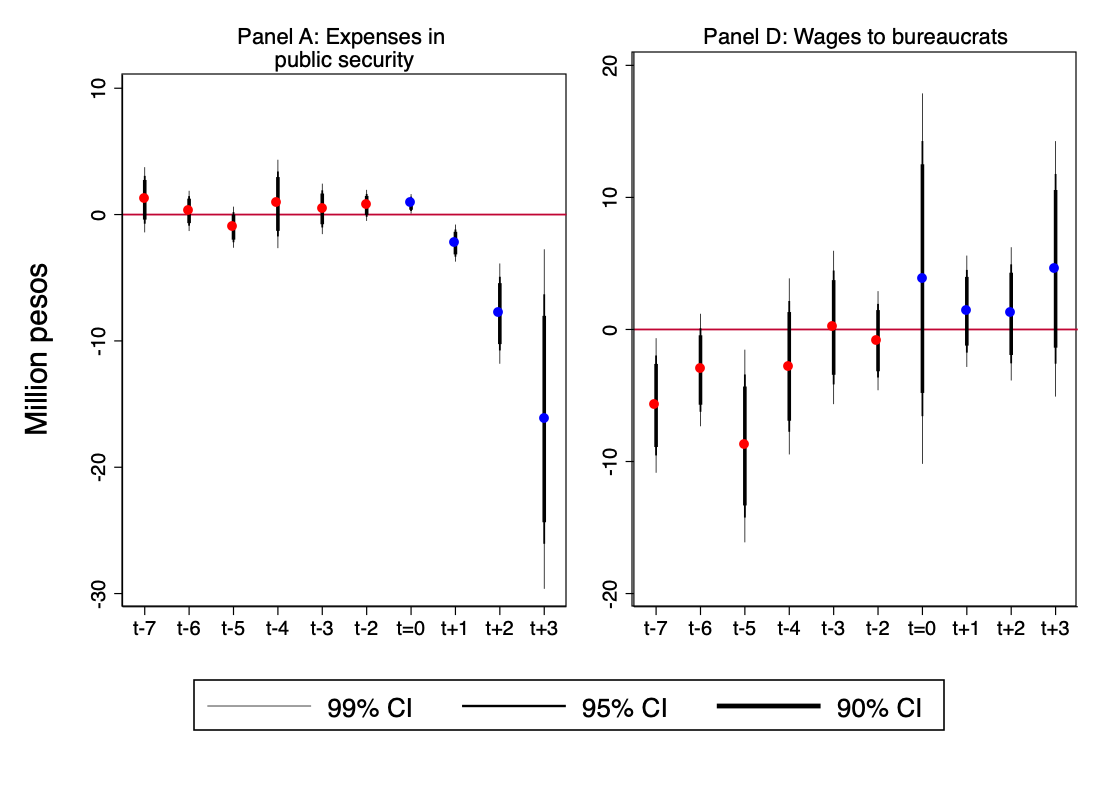
\includegraphics[width=0.9\textwidth]{Figures/expenses_allyears.png}
       \captionsetup{justification=centering}
         
 \textbf{Note:} Figure \ref{fig:expenses} shows the IW estimators following \citet{abraham_sun_2020} for each lead and lag relative to the first year a municipality implemented reelection. Red points are pre-treatment, while blue ones post-treatment. 
                     
\end{figure}   


\section{Consequences of Mayors Taking Charge of Security Policy: Violence \label{sec:unintended}}


What are the results of mayors up for reelection not delegating security policy to more capable agents like the governor? Until now, I have assumed that the public security provision is a more efficient endeavor under the hands of governors who can pool a greater amount of resources, information, skills and expertise than mayors. Moreover, given the high presence of spillovers delegation seems to be the most efficient way to achieve the monopoly of violence \citep{oates_1972}. Figure \ref{fig:as_violence} reports the reduce form IW estimators for each lead and lag relative to the first year a municipality implemented reelection. Results show a negative effect of reelection incentives on violence. On average, from $t$ to $t+3$, homicides per capita increased in 10.4\% using a logarithmic transformation and 6.6\% using the inverse hyperbolic transformation, significant to the 5 and 10\% respectively. As Appendix Figure \ref{fig:robustness_violence} shows, results are robust across multiple specifications including changing the reference period of the reform and adjusting for the small number of clusters (states) using Wild bootstrap. Further validation is provided by the use of \citet{imai_etal_2020} non-parametric generalization of the difference-in-difference estimator that corrects for invalid negative weighting in standard two-way fixed effects models through propensity score matching (see Appendix Figure \ref{fig:matching_violence}). 


\begin{figure}[h] 
\centering
 \caption{Effect of Term Limit Reform on Violence}
 \label{fig:as_violence}
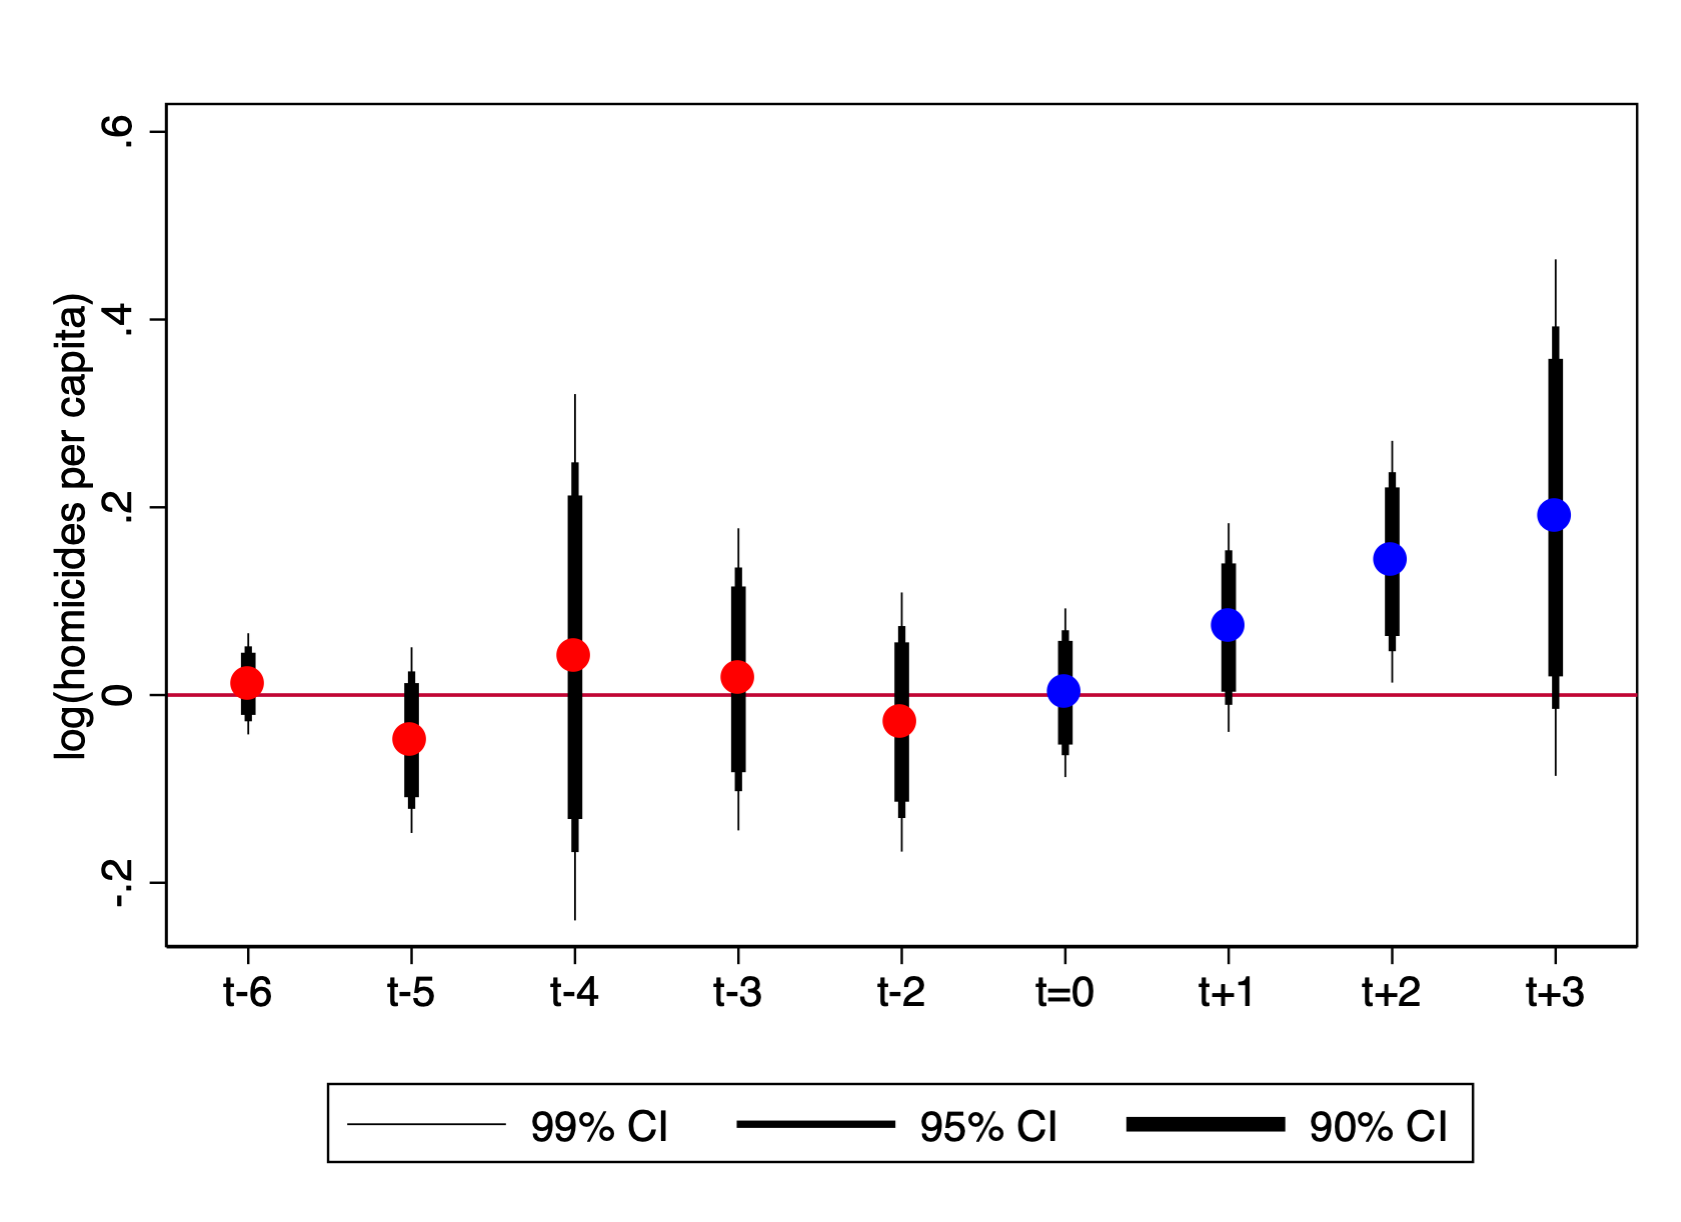
\includegraphics[width=0.9\textwidth]{Figures/catts_homicides.png}
       \captionsetup{justification=centering}
       
 \textbf{Note:} Figure \ref{fig:as_violence} shows the IW estimators following \citet{abraham_sun_2020} for each lead and lag relative to the first year a municipality implemented reelection. Red points are pre-treatment, while blue ones post-treatment. 
    
\end{figure}    

Why do voters do not punish mayors for the increase in violence? Overall, constituents lack the capacity to assess if violence increase in their locality. This problem is even more worrisome when mayors control local news outlets as is the case in the majority of municipalities in Mexico. Moreover, mayors control the spin of local news as many use a media strategy to showcase their competence to fight crime but say it will take a while till peace is achieved. This strategy was widely used by the Felipe Calderon administration in Mexico during his first years in office when violence increased dramatically across the country. Politicians also tend to blame corruption for the increase in violence, arguing that violence increased since corrupt politicians are no longer capable of protecting criminal groups. \citet{ch_2021} further shows that incumbents up for reelection experience a positive incumbency return mainly due to an increase in the resources of the municipality. In other words, increasing resources rather than decreasing welfare due to violence makes citizens sustain mayors in office, while they expect a higher budget or transfer in the future will accrue directly to them. 

\section{Conclusion \label{sec:conclusion}}

This paper studies a classic problem faced by governments with a supra-entity capable of providing and delivering public goods: to delegate or not to delegate. Specifically, it delves into an understudied phenomenon of delegation, the role of reelection incentives. I find that reelection encourages mayors to focus on policies with the highest “electoral yield”—namely, not to delegate public security to the governor. Why? By directly delivering public security mayors can differentiate themselves from others sending a signal to voters on their competence and strong type capable of battling organized crime. This behavior is predominant when citizens are concerned about narcotraffic and when citizens are capable of blaming or rewarding local politicians, i.e. when incumbents seeking reelection are aligned with the party of the governor. This behavior, is a pure credit claiming behavior as in reality mayors do not increase their level of effort to tackle crime, and thus are not responsive to citizens security demands. In other words, in terms of security policy reelection incentives did not strengthen accountability to voters. Since delegation of local security policy to the governor is the most efficient choice in this setting, reelection incentives lead to an inefficient outcome: an increase in violence. These results suggests that reelection incentives may lead incumbents to differentiate themselves by tacking charge of policy at the expense of inefficiency. This makes delegation not only a policy but an electoral decision. 

It is important to acknowledge certain caveats of this paper and avenues for future research. A reason why reelection may decrease delegation to upper-level governments is state capture. %Public good provision entails, sometimes, the interaction with a third player. %For example, incumbents interrelate with firms who compete for procurement bids. In the process, however, incumbents may be captured, changing the market structure and decreasing welfare. This is even more prevalent with longer tenures \citep{coviello_etal_2017}. As noted by  \citet{canen_etal_2020} influence groups are strategic and react to the uncertainty of the political environment by capturing the local apparatus. 
Incumbents may be captured by non-state armed groups who modify local institutions in favor of their self interest \citep{ch_etal_2018}, including a reduction in state-led violence agains them which could be achieved by not delegating security policy to more capable agents like the governor.  Moreover, a more nefarious read of the results of this paper is that incumbents up for reelection  do not delegate policy to the governor to have the capacity to flexibly negotiate terms with criminal groups. This mechanism does not invalidate the differentiation mechanism described in the paper but adds a future mechanism to explore. 

Lastly, is its important to consider that by delegating policy, mayors introduce monitoring to their security forces from another principal -in this case the governor- reducing the potential leeway given to them to overgraze the bribe base through extortions and other rent extraction activities \citep{schleifer_vishny_1993}. They also loose the use of police forces as brokers during elections. Since bureaucrats are important political brokers, especially in clientelistic systems like Mexico \citep{larreguy_etal_2017}, delegation might displease them increasing their chances of shirking for the harvesting of votes.\footnote{For an example of this behavior by police forces in Mexico see \url{https://vanguardia.com.mx/articulo/llevan-acarreados-del-edomex-al-grito-de-pena-en-el-zocalo-por-cuarto-ano-consecutivo}.} A new avenue of research on the electoral behavior of police forces as political brokers could provide new mechanisms on to why mayors choose not to delegate security policy.
           
%this alternative explanation can coexist with mine. 


%BIBLIOGRAPHY -----------------------------------------------
\clearpage
   
%%%%%%%%%%%%
\bibliographystyle{aer} 
\bibliography{References}      

\clearpage
%APPENDIX -----------------------------------------------
\begin{appendix}


%%%%%%%%% Electoral Reform 2014
\section{Political Background of the 2014 Electoral Reform}\label{appendix:reform_backgorund}


It is important to understand the electoral reform political motivation, which involved a bargaining process with the opposition as well as the incorporation of pending laws from the political reform of 2012 under the PAN presidency. In the last year of Felipe Calderon presidency, a political reform was introduced in Congress including a term limit removal for all political actors. This reform was proposed and introduced during the electoral period of that year, increasing political tensions among the incumbent and opposition parties. The PRI -at the time part of the opposition and in control of the lower legislative house- blocked the reform and targeted reelection and the introduction of a second electoral round for the presidential election. 
 
  The 2012 presidential election was won by the coalition ``Alliance for Mexico'' with its presidential candidate Enrique Pena Nieto.\footnote{The PRI won with 38.2\% of total votes, followed by the PRD with 32.6\% and the PAN with 25.390\%.} However, the election suffered multiple electoral irregularities exposed by the national media. Among anomalies, opposition parties led by Andres Manuel Lopez Obrador -the second runner of presidential election and at the time presidential candidate for the left-wing party PRD-, argued PRI's financial expenses above campaign caps and vote-buying practices including the distribution of gift cards from several institutions, including one of the country's largest supermarket chains, Soriana, to voters in the State of Mexico and Mexico city. \citet{cantu_2019} finds not only an effect of the gift cards in PRI electoral return, but a magnitude that increases given proximity of electoral precincts to stores. While the special commission in the Chamber of Deputies found that the PRI invested \$5,200 million pesos in the campaign, an amount 15 times larger than the finance cap of \$336 million pesos, and the Inspection Unit from the Federal Electoral Institute (IFE for its acronym in Spanish) detailed the financing network where Soriana, Banamex, Monex and other firms where involved, the Unit did not point to any law violation. Without a public discussion, the ministers of the Federation Judicial Electoral Tribunal (TEPJF for its acronym in Spanish) deemed the appeal filed by the PRD unfounded and endorsed IFE's  criterion that the PRI was not obliged to register the agreement with Soriana, Banamex or Monex as campaign expenses.\footnote{In his presentation, magistrate Manuel Gonzalez Oropeza stated that the analysis carried by the Inspection Unit showed that ``neither the allegedly hidden financing was accredited individually or jointly" by any member of the PRI. See \url{https://www.jornada.com.mx/2013/01/24/politica/013n2pol} for more detail.} The final resolution of IFE's Council and the TEPJF increased citizens and opposition mistrust on electoral institutions. 

By early 2013, the Pena Nieto administration pushed an aggressive set of reforms to privatize the energy sector and modify the existent fiscal institutions in the country. To increase the probability of success, the PRI with the PAN and PRD, the three main political parties at the time, lead the construction of the Mexican Pact Accord, a series of roundtables intended to negotiate the energy sector reform along a set of structural reforms that had fail to pass through congress due to political gridlocks.\footnote{The PRD was no longer under the Lopez Obrador leadership who left the party to build a new left-wing party called MORENA once the leaders from the PRD agreed to form part of the Mexican Pact Accord.} While the Electoral Reform was not under PRI's set of desired reforms, the opposition utilize it as a bargaining chip to approve those pursued by the PRI \citep{zamitiz_2017}. By the end of May 2013, a roundtable to discuss the electoral reform was installed. Specifically, commitment 94 of the Pact Accord introduced reelection for discussion. However, due to lack of consensus, the Mexican Pact Accord did not submit an electoral reform proposal to Congress and left the bargaining process to the Senate. Two months later, on July 24, 2013, PAN and PRD pushed a political-electoral reform with 36 law changes that included  the creation of a National Electoral Institute (INE for its acronym in Spanish) that would be in charge of federal, state and local elections and reelection for federal and local legislators and mayors. In the words of the current Chairman of the INE, Lorenzo Cordova, ``[w]ith the reform, we went from an electoral model made up of a federal electoral system and thirty-two electoral systems, to a national election system in which a national authority and thirty-two local authorities coexist; a national administrative body was created, with clear powers and powers for local elections, and an authority was created that coordinates and guarantees the same parameters for the application of laws by local authorities, in order to standardize the conditions of the electoral competition in all elections and to promote a more transparent and impartial democracy throughout the country€.\footnote{From Cfr. Compendio de Legislacion Nacional Electoral, Mexico, INE, FEPADE, UNAM, TEPJF, Tomo II, 2014, p. XXXIX.} 


The reaction of governors was not smooth since reelection would limit the influence of governors and local elites on the electoral processes of the 32 states. Strong governors like the priista Eruviel Avila Villegas from the State of Mexico labeled this initiative as ``democratic regression".\footnote{For more detail see ``Regresion democratica, creacion del Instituto Nacional de Elecciones€, La Jornada, 30 de octubre, 2013, p. 15. \url{https://www.20minutos.com.mx/noticia/b82075/regresion-democratica-creacion-del-instituto-nacional-de-elecciones/}} Given the state-level opposition, Senate leaders from the PAN and PRD chose to approve the electoral reform in December 2, 2013, before the energy reform, and thus increased their political grip over the PRI.\footnote{The electoral reform approved by the Senate included reelection for federal legislators and governors for up to 12 years, as well as reelection for local legislators and mayors. Congress, however, modified the proposal removing governors reelection. The electoral reform was approved with 408 votes in favor and 69 against in Congress on December 3, 2013, and weeks later by the Senate due to modifications of the original reform project.} By January 2014, PAN and PRD threatened to back the energy reform  if the PRI did not push local state legislatures from approving the electoral reform, a constraint imposed by the Mexican constitution, which at the time where blocking the reform given pressure from various PRI governors.\footnote{For more detail see Enrique Mendez, ``PAN: estancados, cambios en materia politica por presion de los gobernadores€, La Jornada, 9 de enero de 2014, p. 5., \url{https://jornada.com.mx/2014/01/09/politica/005n3pol}.} The political gridlock led former President Pena Nieto to ``exhort" local legislators to approve the electoral reform. On January 31, 2014, the reform was promulgated by the President and contained three main changes: (1) the creation of the INE; (2) removal of term limits of mayors, local and federal legislators for up to 2 terms; (3) the introduction of a ``party-lock"	where mayors or legislators who wish to reelected could not switch parties. As a result, while voter accountability increased, party control remained unchanged since candidate nominations and campaign funding still depended strongly on them. 
 \clearpage 
  
%%%%%%%%%%%%%%%%%%%%%%%%%%%%%%%%%%%%

\renewcommand{\thetable}{B-\arabic{table}}
\setcounter{table}{0}
 
 \renewcommand{\thefigure}{B-\arabic{figure}}
\setcounter{figure}{0}

\clearpage
\section{Additional Tables and Figures \label{sec:additional_tables}}

\subsection{Descriptive Statistics}

%Table
\begin{table}[H]
\centering 
\caption{Descriptive statistics}
 
\label{tab:descriptive}
\scalebox{0.65}{ 
{
\def\sym#1{\ifmmode^{#1}\else\(^{#1}\)\fi}
\begin{tabular}{l*{1}{ccccc}}
\hline\hline
            &        \textbf{Mean}&  \textbf{SD}&  \textbf{Min}&  \textbf{Max}& \textbf{N}\\
\hline
\emph{Pane A - Security Cooperation Agreements:} 	&		&		&		&		\\
Security Coop. Agreement with governor&        0.28&        0.45&           0&           1&      17,832\\
Security Coop. Agreement with other actors besides the governor&        0.06&        0.24&           0&           1&       6,466\\
Delegate Public Security Provision&        0.29&        0.45&           0&           1&       7,123\\
Delegate Transit Activities&        0.10&        0.30&           0&           1&       7,123\\
Delegate Training of Police Forces&        0.08&        0.27&           0&           1&       4,750\\
Delegate Equipment and Technology&        0.08&        0.26&           0&           1&       4,750\\
Delegate Research Activities&        0.07&        0.26&           0&           1&       4,750\\
Delegate Intelligence Activities&        0.07&        0.26&           0&           1&       4,750\\
Delegate the Unification of Laws and Procedures&        0.08&        0.27&           0&           1&       4,750\\
Delegate Public Security Prevention&        0.08&        0.27&           0&           1&       4,750\\
Reason to delegate: Constitutional Change&        0.12&        0.33&           0&           1&      14,248\\
Reason to delegate: Change in Local Laws&        0.11&        0.31&           0&           1&      14,248\\
Reason to delegate: Constitutional Change&        0.11&        0.31&           0&           1&      14,248\\
Reason to delegate: Need of Professionalization&        0.12&        0.33&           0&           1&      14,248\\
Reason to delegate: Need of Coordination&        0.17&        0.38&           0&           1&      14,248\\
Reason to delegate: Prevalence of Crime&        0.09&        0.29&           0&           1&      14,248\\
Reason to delegate: Other&        0.07&        0.25&           0&           1&      14,248\\


\\
\emph{Panel B - Violence:} 	&		&		&		&		\\
deaths by homicide per capita (INEGI)&       23.99&      128.24&           0&       8,462&      21,375\\
log(deaths by homicide per capita) (INEGI)&       -8.34&        1.04&         -13&        -2.4&      21,375\\
asinh(deaths by homicide per capita) (INEGI)&        2.33&        1.91&           0&         9.7&      21,375\\

\\
\emph{Panel C - Citizens' Preferences:} 	&		&		&		&		\\
Topic that worries most: narcotraffic (for all years)&        0.15&        0.05&           0&         .37&      16,625\\
Topic that worries most: insecurity (for all years)&        0.56&        0.09&           0&         .77&      16,625\\
Topic that worries most: punishment of criminals (for all years)&        0.17&        0.06&           0&         .38&      16,625\\
Topic that worries most: corruption (for all years)&        0.26&        0.04&           0&         .36&      16,625\\
Topic that worries most: poverty (for all years)&        0.34&        0.07&           0&         .52&      16,625\\
Topic that worries most: unemployment (for all years)&        0.40&        0.07&           0&         .57&      16,625\\
Topic that worries most: inflation (for all years)&        0.35&        0.04&           0&         .46&      16,625\\
Topic that worries most: natural disaster (for all years)&        0.05&        0.02&           0&         .12&      16,625\\
Topic that worries most: water scarcity (for all years)&        0.15&        0.04&           0&         .25&      16,625\\
Topic that worries most: health (for all years)&        0.23&        0.03&           0&         .31&      16,625\\
Topic that worries most: education (for all years)&        0.31&        0.05&           0&         .47&      16,625\\

\\
\emph{Panel D - Incumbents' quality:} 	&		&		&		&		\\
Incumbent undergraduate or graduate title (indicator)&        0.06&        0.24&           0&           1&      19,430\\

\\ 
%\emph{Pane B - 2014 Electoral Reform:} 	&		&		&		&		\\
%rel\_year==    -8.0000&        0.02&        0.13&           0&           1&      18,000\\
rel\_year==    -7.0000&        0.02&        0.14&           0&           1&      18,000\\
rel\_year==    -6.0000&        0.06&        0.24&           0&           1&      18,000\\
rel\_year==    -5.0000&        0.11&        0.31&           0&           1&      18,000\\
rel\_year==    -4.0000&        0.11&        0.31&           0&           1&      18,000\\
rel\_year==    -3.0000&        0.11&        0.31&           0&           1&      18,000\\
rel\_year==    -2.0000&        0.11&        0.31&           0&           1&      18,000\\
rel\_year==    -1.0000&        0.11&        0.31&           0&           1&      18,000\\
rel\_year==     0.0000&        0.11&        0.31&           0&           1&      18,000\\
rel\_year==     1.0000&        0.09&        0.29&           0&           1&      18,000\\
rel\_year==     2.0000&        0.09&        0.29&           0&           1&      18,000\\
rel\_year==     3.0000&        0.05&        0.22&           0&           1&      18,000\\


%\\

\\ 
 

\hline\hline
\multicolumn{6}{p{1.3\textwidth}}%{\footnotesize{Note: .        
 % }} \\  

\end{tabular} 
} 
}
\end{table}

\pagebreak

%Table
\begin{table}[H]
\centering 
\caption{Descriptive statistics (continuation)}
 
\label{tab:descriptive2}
\scalebox{0.65}{ 
{
\def\sym#1{\ifmmode^{#1}\else\(^{#1}\)\fi}
\begin{tabular}{l*{1}{ccccc}}
\hline\hline
            &        \textbf{Mean}&  \textbf{SD}&  \textbf{Min}&  \textbf{Max}& \textbf{N}\\
\hline

\emph{Panel E - Mechanisms:} 	&		&		&		&		\\
Topic that worries most: narcotraffic (average pre-treatment)&        0.15&        0.05&           0&         .27&      21,375\\
Topic that worries most: insecurity (average pretreatment)&        0.52&        0.08&           0&         .68&      21,375\\
Topic that worries most: punishment of criminals (average pretreatment)&        0.12&        0.02&           0&         .19&      21,375\\
Topic that worries most: poverty (average pretreatment)&        0.37&        0.07&           0&          .5&      21,375\\
Topic that worries most: unemployment (average pretreatment)&        0.46&        0.04&           0&         .52&      21,375\\
Topic that worries most: inflation (average pretreatment)&        0.37&        0.03&           0&         .41&      21,375\\
Topic that worries most: natural disaster (average pretreatment)&        0.05&        0.01&           0&        .088&      21,375\\
Topic that worries most: water scarcity (average pretreatment)&        0.15&        0.03&           0&          .2&      21,375\\
Topic that worries most: corruption (average pretreatment)&        0.24&        0.04&           0&         .34&      21,375\\
Topic that worries most: health (average pretreatment)&        0.24&        0.03&           0&         .29&      21,375\\
Topic that worries most: education (average pretreatment)&        0.31&        0.06&           0&          .4&      21,375\\
Trust in Municipal Security Forces&        0.21&        0.05&           0&          .4&      21,375\\
Trust in State Security Forces&        0.22&        0.05&           0&         .37&      21,375\\
Trust in Federal Security Forces, including the military&        0.55&        0.16&           0&         .77&      21,375\\
Identify Municipal Security Forces&        0.70&        0.06&           1&         .87&      21,375\\
Identify State Security Forces&        0.51&        0.07&           0&          .7&      21,375\\
Identify Federal Security Forces, including the military&        0.53&        0.08&           0&         .75&      21,375\\
Corruption of Municipal Security Forces&        1.24&        0.15&           1&         1.7&      21,375\\
Corruption of State Security Forces&        1.24&        0.14&           1&         1.6&      21,375\\
Corruption of Federal Security Forces, including the military&        1.07&        0.14&           1&         1.6&      21,375\\
Efficiency of Municipal Security Forces&        0.24&        0.06&           0&         .42&      21,375\\
Efficiency of State Security Forces&        0.25&        0.06&           0&         .41&      21,375\\
Efficiency of Federal Security Forces, including the military&        0.57&        0.15&           0&         .78&      21,375\\
Detained by local police per capita (in flagrancy, SNSP)&       10.29&      133.10&           0&      11,408&      21,375\\
log(Detained by local police per capita) (in flagrancy, SNSP)&       -9.06&        1.32&         -14&        -2.2&      21,375\\
log(heroine kg), SEDENA&        0.01&        0.15&           0&         5.4&      21,375\\
log(meth kg), SEDENA&        0.05&        0.48&           0&          10&      21,375\\
log(cocaine kg), SEDENA&        0.04&        0.36&           0&         7.8&      21,375\\
log(poppy kg), SEDENA&        0.19&        0.82&           0&         8.8&      21,375\\
log(laboratories erradicated), SEDENA&        0.02&        0.17&           0&         4.1&      21,375\\
 
\\
\emph{Panel F - Controls:} 	&		&		&		&		\\
Population (INEGI and CONAPO projections)&      53,389&     141,924&         409&   1,714,709&       2,227\\
 
Winning margin: first - second runner (governor)&        0.15&        0.13&           0&           1&      21,375\\
alignment with federal executive=1; 0 otherwise&        0.77&        0.42&           0&           1&      17,962\\
alignment with state executive=1; 0 otherwise&        0.37&        0.48&           0&           1&      17,962\\
Winning margin: first - second runner&        0.11&        0.11&           0&           1&      17,962\\
PAN mayor=1; 0 otherwise&        0.29&        0.46&           0&           1&      17,962\\
PRI mayor=1; 0 otherwise&        0.46&        0.50&           0&           1&      17,962\\
Incidence of Cartel Presence&        0.22&        0.35&           0&           1&      21,375\\

\\ 
 
    
\hline\hline
\multicolumn{6}{p{1.3\textwidth}}%{\footnotesize{Note: .        
 % }} \\  

\end{tabular} 
} 
}
\end{table}

\pagebreak
   
\subsection{Main Results}
\begin{table}[H]\def\sym#1{\ifmmode^{#1}\else\(^{#1}\)\fi}
\centering
\caption{Effect of 2014 Term Limit Reform on Security Cooperation Agreements signed with the Governor, 2010-2018}
\label{tab:as_agreements}
\scalebox{0.75}{
\begin{tabular}{lcc}
\hline \hline
\\ \multicolumn{3}{l}{Dependent variable:}\\
& \multicolumn{2}{c}{Security Cooperation Agreement} \\
& \multicolumn{2}{c}{w/ Governor$^{a}$} \\

& \multicolumn{1}{c}{(1)} & \multicolumn{1}{c}{(2)} \\
\cmidrule(lrr){2-2}  \cmidrule(lrr){3-3}\\
\addlinespace
Lag 7 years &      $ 0.1123^{} $ &  $ 0.1123^{} $   \\
& ($ 0.1709$) & ($ 0.7117 $) \\
Lag 6 years &          $ -0.0383^{} $ &   $ -0.0383^{} $  \\
& ($ 0.0579$) & ($ 0.2458 $) \\
Lag 5 years &        $ -0.0848^{} $ &   $ -0.0848^{} $ \\
& ($ 0.0846$) & ($ 0.2404 $) \\
Lag 4 years &         $ 0.0751^{} $ &      $ 0.0751^{} $  \\
& ($ 0.3174$) & ($ 0.2890 $) \\
Lag 3 years &        $ 0.2088^{} $ &     $ 0.2088^{} $ \\
& ($ 0.2603$) & ($ 0.2139 $) \\
Lag 2 years &        $ 0.0044^{} $ &    $ 0.0044^{} $  \\
& ($ 0.1583$) & ($ 0.2139 $) \\
Reform, time 0 &        $ -0.2446^{***} $ &     $ -0.2446^{***} $ \\
& ($ 0.0475$) & ($ 0.0685 $) \\
Lead 1 year &         $ -0.4154^{***} $ &       $ -0.4154^{***} $ \\
& ($ 0.0610$) & ($ 0.0610 $) \\
Lead 2 years &         $ -0.4259^{***} $ &      $ -0.4259^{***} $  \\
& ($ 0.0571$) & ($ 0.0571 $) \\
Lead 3 years &        $ -0.5931^{***} $ &     $ -0.5931^{***} $ \\
& ($ 0.0604$) & ($ 0.0604 $) \\
\addlinespace
Observations       &                 12,173        &          12,173  \\
R-squared        &              0.4545        &           0.4545   \\
Mun. FEs       &     \checkmark         &  \checkmark    \\
Year. FEs       &     \checkmark         &  \checkmark   \\
Controls$^b$   &      \checkmark       &      \checkmark    \\
Cohort weighted   &   \checkmark       &   \checkmark    \\
WILD CI   &          &   \checkmark    \\
Aggregate effect        &           $   -0.4197^{***} $        &           $-0.4197^{***} $    \\
SE (aggregate eff.)        &              0.0457        &           0.0473   \\
\hline \hline
\multicolumn{3}{p{0.6\textwidth}}{\footnotesize{Notes: Coefficients show IW estimators following \citet{abraham_sun_2020}. Two relative time periods (lag 8 and 1) are removed to avoid collinearity problems noted by \citet{abraham_sun_2020}. Standard errors in parentheses are clustered at the state level, with the following significance-level: $^{***}$ 1\%; $^{**}$ 5\%; and $^*$ 10\%, that refer to two-sided t-test with the null hypothesis equal to 0 for each relative time period. $^a$ Refers to security cooperation agreements signed with the Governor. $^b$ Pretreatment controls include: governor winning margin; party alignment with the President;  party alignment with the Governor; municipal winning margin; logged population; logged organized crime related deaths; and Cartel presence.}} \\
\end{tabular}
} 
\end{table}
    
 
 \clearpage
\subsection{Robustness}

\begin{table}[htbp]\def\sym#1{\ifmmode^{#1}\else\(^{#1}\)\fi}
\centering
\caption{Effect of 2014 Term Limit Reform on Signing Security Cooperation Agreements, Average Effect }
\label{tab:as_aggregate}
\scalebox{0.7}{
\begin{tabular}{lcccc}
\hline \hline
\\ \multicolumn{3}{l}{Dependent variable: Sign Security Cooperation Agreement w/ Governor}\\
Model: & CATTs & CATTs w/ WILD CIs & Change ref. period (t=0) & Trim $<$ t-4 \\
& \multicolumn{1}{c}{(1)} & \multicolumn{1}{c}{(2)} & \multicolumn{1}{c}{(3)}  & \multicolumn{1}{c}{(4)}  \\
\cmidrule(lrr){2-2}  \cmidrule(lrr){3-3}  \cmidrule(lrr){4-4} \cmidrule(lrr){5-5}\\
\addlinespace
Reform Average Effect (from t to t+3)       & $-0.4197^{***} $$ & $-0.4197 ^{***} $$ & $-0.4622 ^{**} $$ & $-0.3559 ^{***} $$   \\
& (0.0457( & (0.0473)  & (0.1977) & (0.0468)  \\
\addlinespace
Observations       &      12,173 &      12,173 &      12,173 &      12,173 \\
R-squared         & 0.4545 & 0.4545 & 0.4545 & 0.4544 \\
Mun. FEs       &     \checkmark         &  \checkmark &     \checkmark         &  \checkmark     \\
Year. FEs       &     \checkmark         &  \checkmark  &     \checkmark         &  \checkmark \\
Controls$^b$   &      \checkmark       &      \checkmark &      \checkmark       &      \checkmark    \\
Cohort weighted   &   \checkmark       &   \checkmark  &   \checkmark       &   \checkmark  \\
Parallel trend holds   &   \checkmark       &   \checkmark  &   \checkmark       &   \checkmark   \\
\hline \hline
\multicolumn{5}{p{1.3\textwidth}}{\footnotesize{Notes: Coefficients show IW estimators following \citet{abraham_sun_2020}. Two relative time periods (lag 8 and 1) are removed to avoid collinearity problems noted by \citet{abraham_sun_2020} except for the specification that trims periods prior to t-4. Standard errors in parentheses are clustered at the state level, with the following significance-level: $^{***}$ 1\%; $^{**}$ 5\%; and $^*$ 10\%, that refer to two-sided t-test with the null hypothesis equal to 0 for each relative time period. $^b$ State-level controls include governor winning margin in last pre-treatment election and an indicator of whether the governor's party is the same as the federal incumbent party.}} \\
\end{tabular}
}
\end{table}
 

\begin{table}[htbp]\def\sym#1{\ifmmode^{#1}\else\(^{#1}\)\fi}
\centering
\caption{Effect of 2014 Term Limit Reform on the likelihood of signing Security Cooperation Agreements, \citet{chaisemarting_etal_2019} correction}
\label{tab:chaisemartin_agreements}
\scalebox{1}{
\begin{tabular}{lcc}
\hline \hline
\\ \multicolumn{3}{l}{Dependent variable:}\\
& \multicolumn{1}{c}{Agreement A} & \multicolumn{1}{c}{Agreement B$^{a}$} \\
& \multicolumn{1}{c}{(1)} & \multicolumn{1}{c}{(2)} \\
\cmidrule(lrr){2-2}  \cmidrule(lrr){3-3}\\
\addlinespace
t-6 &          $ -0.0645^{} $ &   $ -0.0645^{} $  \\
& ($ 0.0399$) & ($ 0.8961 $) \\
t-5 &        $ -0.2071^{**} $ &   $ -0.2071^{} $ \\
& ($ 0.0751$) & ($ 2.6703 $) \\
t-4 &         $ -0.0712^{} $ &      $ -0.0712^{} $  \\
& ($ 0.1733$) & ($ 1.2658 $) \\
t-3 &        $ 0.1037^{} $ &     $ 0.1037^{} $ \\
& ($ 0.1362$) & ($ 0.3138 $) \\
t-2 &        $ -0.0251^{} $ &    $ -0.0251^{} $  \\
& ($ 0.1157$) & ($ 0.3138 $) \\
t-1 &        $ -0.0738^{} $ &     $ -0.0738^{} $ \\
& ($ 0.0918$) & ($ 1.6557 $) \\
t+1 &         $ -0.2837^{} $ &       $ -0.2837^{} $ \\
& ($ 0.2012$) & ($ 0.2012 $) \\
t+2 &         $ -0.6165^{**} $ &      $ -0.6165^{**} $  \\
& ($ 0.2330$) & ($ 0.2330 $) \\
t+3 &        $ -0.4813^{*} $ &     $ -0.4813^{*} $ \\
& ($ 0.2641$) & ($ 0.2641 $) \\
\addlinespace
Observations       &                 12,173        &          12,173  \\
R-squared        &              0.4542        &           0.4542   \\
Mun. FEs       &     \checkmark         &  \checkmark    \\
Year. FEs       &     \checkmark         &  \checkmark   \\
Controls$^b$   &      \checkmark       &      \checkmark    \\
Cohort weighted   &   \checkmark       &   \checkmark    \\
WILD CI   &          &   \checkmark    \\
Aggregate effect        &              -0.4605        &           -0.4605   \\
SE (aggregate eff.)        &              0.1973        &           0.1973   \\
p-value(aggregate eff.)       &              0.0273        &           0.0273   \\
\hline \hline
\multicolumn{3}{p{0.8\textwidth}}{\footnotesize{Notes: Coefficients show IW estimators following \citet{abraham_sun_2020}. Two relative time periods (lag 8 and 1) are removed to avoid collinearity problems noted by \citet{abraham_sun_2020}. Standard errors in parentheses are clustered at the state level, with the following significance-level: $^{***}$ 1\%; $^{**}$ 5\%; and $^*$ 10\%, that refer to two-sided t-test with the null hypothesis equal to 0 for each relative time period. $^a$ Refers to the inverse hyperbolic sine transformation. $^b$ State-level controls include governor winning margin in last pre-treatment election and an indicator of whether the governor's party is the same as the federal incumbent party.}} \\
\end{tabular}
}
\end{table}
  
    
 \begin{table}[htbp]\def\sym#1{\ifmmode^{#1}\else\(^{#1}\)\fi}
\centering
\caption{Effect of Term Limit Reform on Security Cooperation Agreements signed with the Governor, trimming periods}
\label{tab:as_agreements_trim}
\scalebox{1}{
\begin{tabular}{lcc}
\hline \hline
\\ \multicolumn{3}{l}{Dependent variable:}\\
& \multicolumn{2}{c}{Security Cooperation Agreement} \\
& \multicolumn{2}{c}{w/ Governor$^{a}$} \\
& \multicolumn{1}{c}{(1)} & \multicolumn{1}{c}{(2)} \\
\cmidrule(lrr){2-2}  \cmidrule(lrr){3-3}\\
\addlinespace
t-4 years &         $ 0.1961^{} $ &      $ 0.1961^{} $  \\
& ($ 0.2680$) & ($ 0.8260 $) \\
t-3 &        $ 0.2193^{} $ &     $ 0.2193^{} $ \\
& ($ 0.2070$) & ($ 0.2702 $) \\
t-2 &        $ 0.0370^{} $ &    $ 0.0370^{} $  \\
& ($ 0.1546$) & ($ 0.2702 $) \\
t=0 (Reform) &        $ -0.3057^{***} $ &     $ -0.3057^{} $ \\
& ($ 0.0682$) & ($ 0.4093 $) \\
t+1 &         $ -0.2858^{***} $ &       $ -0.2858^{} $ \\
& ($ 0.0725$) & ($ 0.2610 $) \\
t+2 &         $ -0.2389^{***} $ &      $ -0.2389^{} $  \\
& ($ 0.0823$) & ($ 0.2369 $) \\
t+3  &        $ -0.5931^{***} $ &     $ -0.5931^{***} $ \\
& ($ 0.0604$) & ($ 0.0715 $) \\
\addlinespace
Observations       &                 12,173        &          12,173  \\
R-squared        &              0.4544        &           0.4544   \\
Mun. FEs       &     \checkmark         &  \checkmark    \\
Year. FEs       &     \checkmark         &  \checkmark   \\
Controls$^b$   &      \checkmark       &      \checkmark    \\
Cohort weighted   &   \checkmark       &   \checkmark    \\
WILD CI   &   \checkmark       &   \checkmark    \\
Aggregate effect        &              $-0.3559^{***} $     &          $ -0.3559^{**} $     \\
SE (aggregate eff.)        &              0.0468        &           0.1395   \\
\hline \hline
\multicolumn{3}{p{0.6\textwidth}}{\footnotesize{Notes: Coefficients show IW estimators following \citet{abraham_sun_2020}. I trimmed the periods lag 8, 7, 6 and 5, and removed the period 1 to avoid collinearity problems noted by \citet{abraham_sun_2020}. Standard errors in parentheses are clustered at the state level, with the following significance-level: $^{***}$ 1\%; $^{**}$ 5\%; and $^*$ 10\%, that refer to two-sided t-test with the null hypothesis equal to 0 for each relative time period. $^a$ Refers to security cooperation agreements signed with the Governor. $^b$ Pretreatment controls include: governor winning margin; party alignment with the President;  party alignment with the Governor; municipal winning margin; logged population; logged organized crime related deaths; and Cartel presence.}} \\
\end{tabular}
}
\end{table}
  

  \begin{table}[htbp]\def\sym#1{\ifmmode^{#1}\else\(^{#1}\)\fi}
\centering
\caption{Effect of 2014 Term Limit Reform on the likelihood of signing Security Cooperation Agreements}
\label{tab:chaisemartin}
\scalebox{1}{
\begin{tabular}{lcc}
\hline \hline
\\ \multicolumn{3}{l}{Dependent variable:}\\
& \multicolumn{1}{c}{Agreement A} & \multicolumn{1}{c}{Agreement B$^{a}$} \\
& \multicolumn{1}{c}{(1)} & \multicolumn{1}{c}{(2)} \\
\cmidrule(lrr){2-2}  \cmidrule(lrr){3-3}\\
\addlinespace
Lag 5 years &        $     .^{} $ &     $     .^{} $ \\
& ($     .$) & ($     . $) \\
Lag 4 years &        $     .^{} $ &     $     .^{} $ \\
& ($     .$) & ($     . $) \\
Lag 3 years &        $ -0.000^{} $ &     $ -0.035^{} $ \\
& ($ 0.466$) & ($ 0.054 $) \\
Lag 2 years &        $ -0.000^{} $ &     $ -0.006^{} $ \\
& ($ 0.075$) & ($ 0.053 $) \\
Reform, time 0 &        $ 0.057^{} $ &     $ -0.200^{**} $ \\
& ($ 0.167$) & ($ 0.094 $) \\
Lead 1 year &         $ -0.091^{} $ &       $ -0.256^{} $ \\
& ($ 0.898$) & ($ 0.296 $) \\
Lead 2 years &         $ -0.182^{} $ &      $ -0.211^{} $  \\
& ($ 0.725$) & ($ 0.189 $) \\
\addlinespace
Controls$^b$   &    \checkmark      &   \checkmark    \\
\hline \hline
\multicolumn{3}{p{0.8\textwidth}}{\footnotesize{Notes: Coefficients show corrected estimators following \citet{chaisemarting_etal_2019}. Standard errors in parentheses are clustered at the state level, with the following significance-level: $^{***}$ 1\%; $^{**}$ 5\%; and $^*$ 10\%.$^a$ Secondary version of security cooperation agreements. $^b$ State-level controls include governor winning margin in last pre-treatment election and an indicator of whether the governor's party is the same as the federal incumbent party.}} \\
\end{tabular}
}
\end{table}
  
      
     \clearpage
      
\begin{figure}[H] 
\centering
 \caption{Effect of Term Limit Reform on Security Cooperation Agreements signed with the Governor, propensity score matching on pretreatment covariates}
 \label{fig:matching}
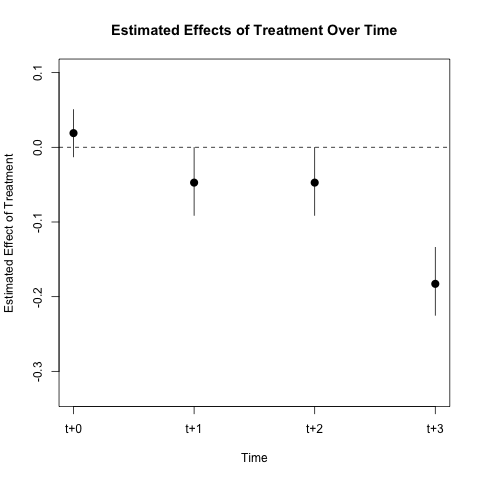
\includegraphics[width=0.9\textwidth]{Figures/acuerdo_gobestatal.png}
       \captionsetup{justification=centering}
       
        
 \textbf{Note:} Figure \ref{fig:matching} produced by propensity score matching that adjust for the treatment and covariate histories during the 5 year periods prior to the treatment. I report 95\% bootstrap confidence intervals clustered at the state level. Covariates include those used to generate Figure \ref{fig:event_study_agreements}. 

\end{figure}   
 
 \clearpage 
\begin{figure}[H] 
\centering
 \caption{Effect of Term Limit Reform on Security Cooperation Agreements signed with the Governor, 2010-2018}
 \label{fig:chaisemarting_agreements}
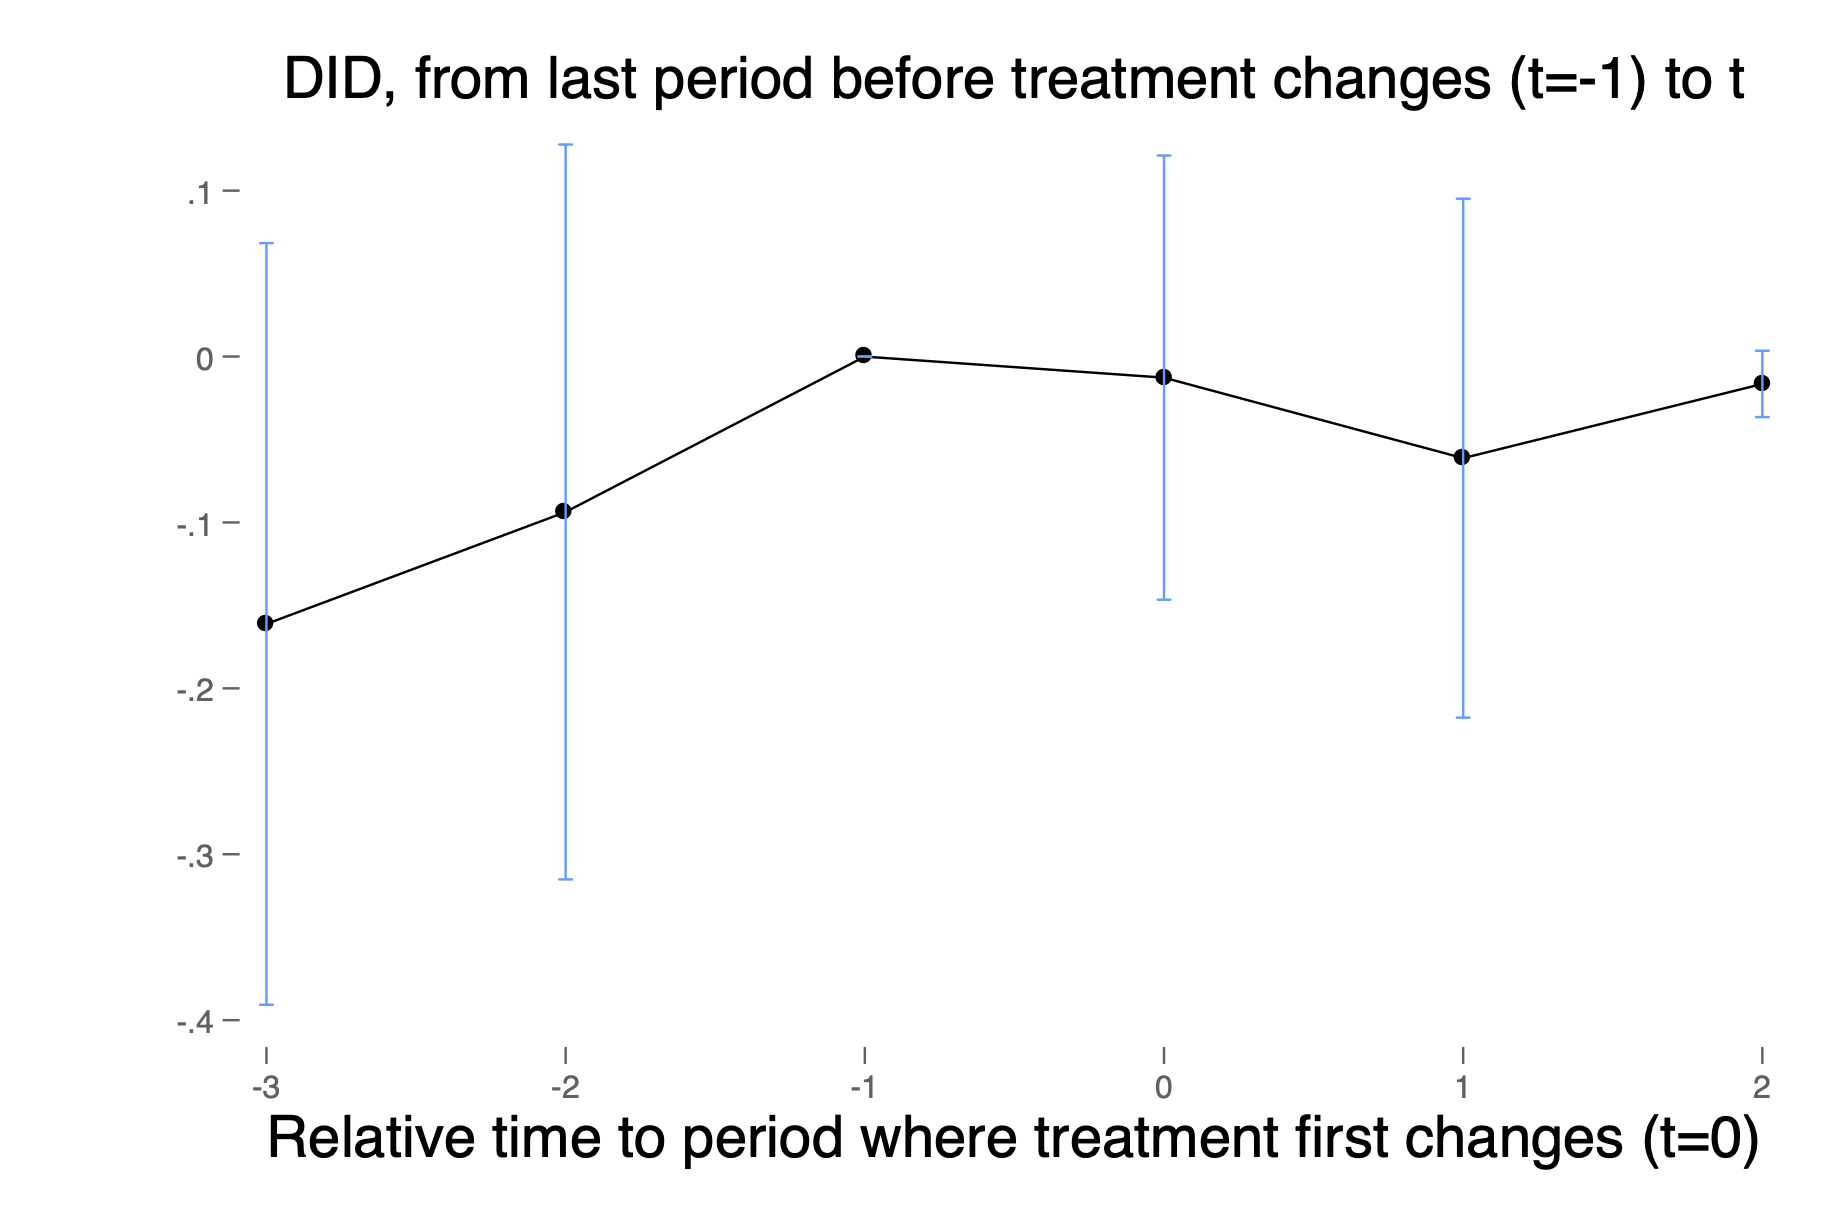
\includegraphics[width=0.9\textwidth]{Figures/chaisemartin_acuerdo_estcom.png}
       \captionsetup{justification=centering}
\end{figure}   

  %\begin{table}[htbp]\def\sym#1{\ifmmode^{#1}\else\(^{#1}\)\fi}
\centering
\caption{Comparison: Security Cooperation Agreements with Governor vs. Other Actors, 2014-2018}
\label{tab:as_comparison_agreements}
\scalebox{1}{
\begin{tabular}{lcc}
\hline \hline
\\ \multicolumn{3}{l}{Dependent variable: Security Cooperation Agreement}\\
& w/ Governor &  w/ Other Political Actors$^a$\\
& \multicolumn{1}{c}{(1)} & \multicolumn{1}{c}{(2)} \\
\cmidrule(lrr){2-2}  \cmidrule(lrr){3-3}\\
\addlinespace
Lag 4 years &         $ 0.0197^{} $ &      $ -0.0326^{} $  \\
& ($ 0.3292$) & ($ 0.0763 $) \\
Lag 3 years &        $ -0.0102^{***} $ &     $ 0.2193^{} $ \\
& ($ 0.0000$) & ($ 0.2702 $) \\
Lag 2 years &        $ 0.1418^{} $ &    $ -0.0648^{} $  \\
& ($ 0.1318$) & ($ 0.0524 $) \\
Reform, time 0 &        $ 0.0064^{} $ &     $ -0.0089^{} $ \\
& ($ 0.0354$) & ($ 0.0069 $) \\
Lead 1 year &         $ -0.2230^{***} $ &       $ -0.2858^{} $ \\
& ($ 0.0435$) & ($ 0.2610 $) \\
Lead 3 years &        $ -0.5921^{***} $ &     $ 0.1665^{} $ \\
& ($ 0.0708$) & ($ 0.1040 $) \\
\addlinespace
Observations       &                  4,382        &           4,382  \\
R-squared        &              0.6434        &           0.5469   \\
Mun. FEs       &     \checkmark         &  \checkmark    \\
Year. FEs       &     \checkmark         &  \checkmark   \\
Controls$^b$   &      \checkmark       &      \checkmark    \\
Cohort weighted   &   \checkmark       &   \checkmark    \\
WILD CI   &          &       \\
Aggregate effect        &              $-0.2696^{***} $$         &            $0.0796^{} $$   \\
SE (aggregate eff.)        &              (0.0339)       &           (0.0491)   \\
\hline \hline
\multicolumn{3}{p{0.7\textwidth}}{\footnotesize{Notes: Coefficients show IW estimators following \citet{abraham_sun_2020}. Two relative time periods (lag 5 and 1) are removed to avoid collinearity problems noted by \citet{abraham_sun_2020}. Standard errors in parentheses are clustered at the state level, with the following significance-level: $^{***}$ 1\%; $^{**}$ 5\%; and $^*$ 10\%, that refer to two-sided t-test with the null hypothesis equal to 0 for each relative time period. $^a$ Refers primarily to the President but could include Governors and mayors from other states or other municipalities from the same state. $^b$ Pretreatment controls include: governor winning margin; party alignment with the President;  party alignment with the Governor; municipal winning margin; logged population; logged organized crime related deaths; and Cartel presence.}} \\
\end{tabular}
}
\end{table}
   
  
  \begin{table}[htbp]\def\sym#1{\ifmmode^{#1}\else\(^{#1}\)\fi}
\centering
\caption{Effect of 2014 Term Limit Reform on the likelihood of signing Security Cooperation Agreements,  by type}
\label{tab:comparison_fed_estatal}
\scalebox{1}{
\begin{tabular}{lcccc}
\hline \hline
\\ \multicolumn{3}{l}{Dependent variable:}\\
& \multicolumn{2}{c}{Security Cooperation Agreement w/ Governor$^{a}$} & \multicolumn{2}{c}{Security Cooperation Agreement w/ Other$^{b}$} \\
& \multicolumn{1}{c}{(1)} & \multicolumn{1}{c}{(2)} & \multicolumn{1}{c}{(3)} & \multicolumn{1}{c}{(4)} \\
\cmidrule(lrr){2-3}  \cmidrule(lrr){4-5}\\
\addlinespace
t-4 &         $ 0.3497^{} $ &         $ 0.0193^{} $ &     $ -0.2763^{} $ &   $ -0.0326^{} $  \\
& ($ 1.8038$) & ($ 0.3316$) & ($ 0.5842$)  & ($ 0.0761 $) \\
t-3 &         $ -0.7355^{} $ &        $ -0.0102^{***} $  &     $ 0.2469^{} $ &     $ 0.2206^{} $ \\
& ($ 37.4159$) & ($ 0.0000$) & ($ 15.0281$) & ($ 0.2702 $) \\
t-2 &         $ 0.3861^{} $ &        $ 0.1420^{} $  &     $ -0.1496^{} $ &    $ -0.0649^{} $  \\
& ($ 0.3279$) & ($ 0.1323$) & ($ 0.1250$) & ($ 0.0524 $) \\
Reform (t=0) &         $ 0.2233^{***} $ &        $ 0.0065^{} $  &     $ -0.0599^{**} $  &     $ -0.0089^{} $ \\
& ($ 0.0581$) & ($ 0.0353$) & ($ 0.0273$) & ($ 0.0070 $) \\
t+1 &         $ -0.2198^{**} $ &         $ -0.2230^{***} $  &     $ 0.1148^{} $ &       $ -0.2845^{} $ \\
& ($ 0.0930$) & ($ 0.0435$) & ($ 0.0904$) & ($ 0.2602 $) \\
t+3 &         $ -0.5915^{***} $ &        $ -0.5921^{***} $ &     $ 0.1660^{*} $  &     $ 0.1665^{} $ \\
& ($ 0.0783$) & ($ 0.0708$) & ($ 0.0953$) & ($ 0.1040 $) \\
\addlinespace
Observations   &                  4,382     &                  4,382  &                  4,382        &           4,382  \\
R-squared      &              0.6433    &              0.6434   &            0.5469        &           0.5469   \\
Mun. FEs       &     \checkmark         &  \checkmark   &     \checkmark         &  \checkmark   \\
Year. FEs       &     \checkmark         &  \checkmark  &     \checkmark         &  \checkmark   \\
Controls$^b$   &      \checkmark       &      \checkmark   &      \checkmark       &      \checkmark   \\
Cohort weighted   &          &   \checkmark   &          &   \checkmark   \\
WILD CI  &     \checkmark         &  \checkmark   &     \checkmark         &  \checkmark   \\
Aggregate effect     &              $-0.213^{***} $$    &        $-0.2696^{***} $$      &            $0.069^{} $$   &       $0.0796^{} $$   \\
SE (aggregate eff.)      &              0.034   &              0.0339    &              0.045       &           0.0491   \\
\hline \hline
\multicolumn{5}{p{1.2\textwidth}}{\footnotesize{Notes: Coefficients in columns (2) and (4) show IW estimators following \citet{abraham_sun_2020}. In those models, two relative time periods (lag 8 and 1) are removed to avoid collinearity problems noted by \citet{abraham_sun_2020}. Standard errors in parentheses are clustered at the state level, with the following significance-level: $^{***}$ 1\%; $^{**}$ 5\%; and $^*$ 10\%, that refer to two-sided t-test with the null hypothesis equal to 0 for each relative time period. $^a$ Refers to security cooperation agreements signed with the governor only. $^b$ Refers to security cooperation agreements signed with other instituions but not the governor. $^c$ State-level controls include governor winning margin in last pre-treatment election and an indicator of whether the governor's party is the same as the federal incumbent party.}} \\
\end{tabular}
}
\end{table}
   
 
 
\def\sym#1{\ifmmode^{#1}\else\(^{#1}\)\fi}
\begin{table}[htbp]\def\sym#1{\ifmmode^{#1}\else\(^{#1}\)\fi}
\centering
\caption{Test on selection on unobservables}
\label{tab:unobservables}
\begin{tabular}{l*{1}{c}}
\hline \hline
&\multicolumn{1}{c}{(1)}         \\
\addlinespace
Fitted value&      0.1312         \\
            &    (0.0780)         \\
\addlinespace
Observations&      10,668         \\
R2          &       0.459         \\
Mun. FE     &      \checkmark               \\
Year FE     &      \checkmark               \\
State Cluster S.E.&     \checkmark                \\
\hline \hline 
\multicolumn{2}{p{0.6\textwidth}}{\footnotesize{Notes: I follow \citet{altonji_etal_2005} to check if unobserved variation is likely to explain the signing of security cooperation agreements with the Governor by mayors. To do so, I regress the treatment (whether the municipality held reelection) on all the available covariates used for Figure \ref{fig:event_study_agreements}.} I then take the fitted value from the regression and use it to predict each outcome, this time including unit and year fixed effects. This test suggests that – under the assumption that observables are representative of unobservables – selection on unobservables is not driving the results.} \\
\end{tabular}
\end{table} 

\clearpage 


\begin{comment}
\begin{figure}[H]
\centering
\caption{Effect of Electoral Reform on Security Cooperation Agreement using non parametric methods\\ -95\% confidence intervals-} 
\label{fig:non_did_agreement}
\begin{center} 
\begin{center} 
	{\textbf Figure A: Generalized Synthetic Control following \citet{xu_2016} }
\end{center}
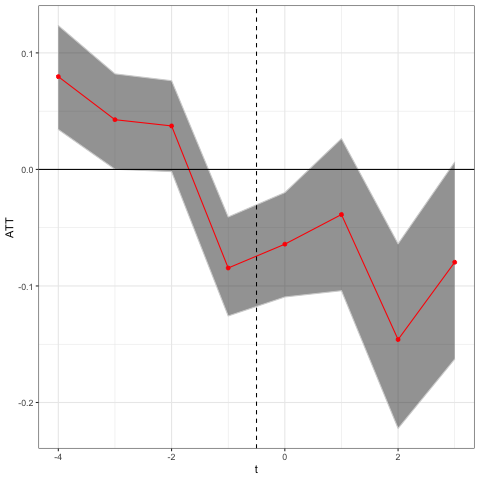
\includegraphics[width=0.55\textwidth]{Figures/gsynth_wcov_acuerdo.png}

\begin{center}
	{\textbf Figure B: Matrix Completion following \citet{Athey, Bayati, Doudchenko, Imbens, and Khosvari}
\end{center}
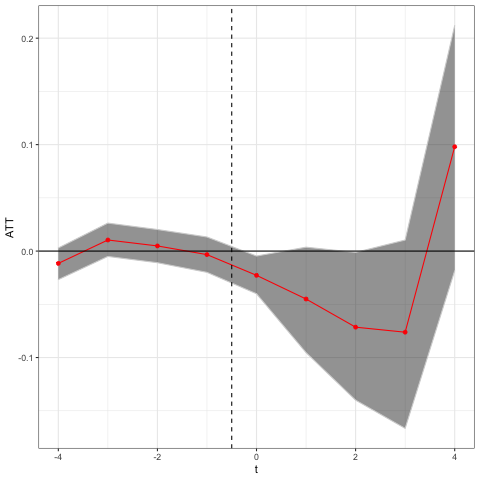
\includegraphics[width=0.55\textwidth]{Figures/matrix_completion.png}
       \captionsetup{justification=centering}
       \\
 %{\textbf Note: 95\% confidence intervals estimated using 1,000 bootstrap replications.} .   
\end{figure}      
\end{comment}


\clearpage

\subsection{Mechanisms}

\begin{figure}[H] 
\centering
 \caption{Effect of 2014 Term Limit Reform on Motives to Sign Security Agreements w/ Governor}
 \label{fig:motives}
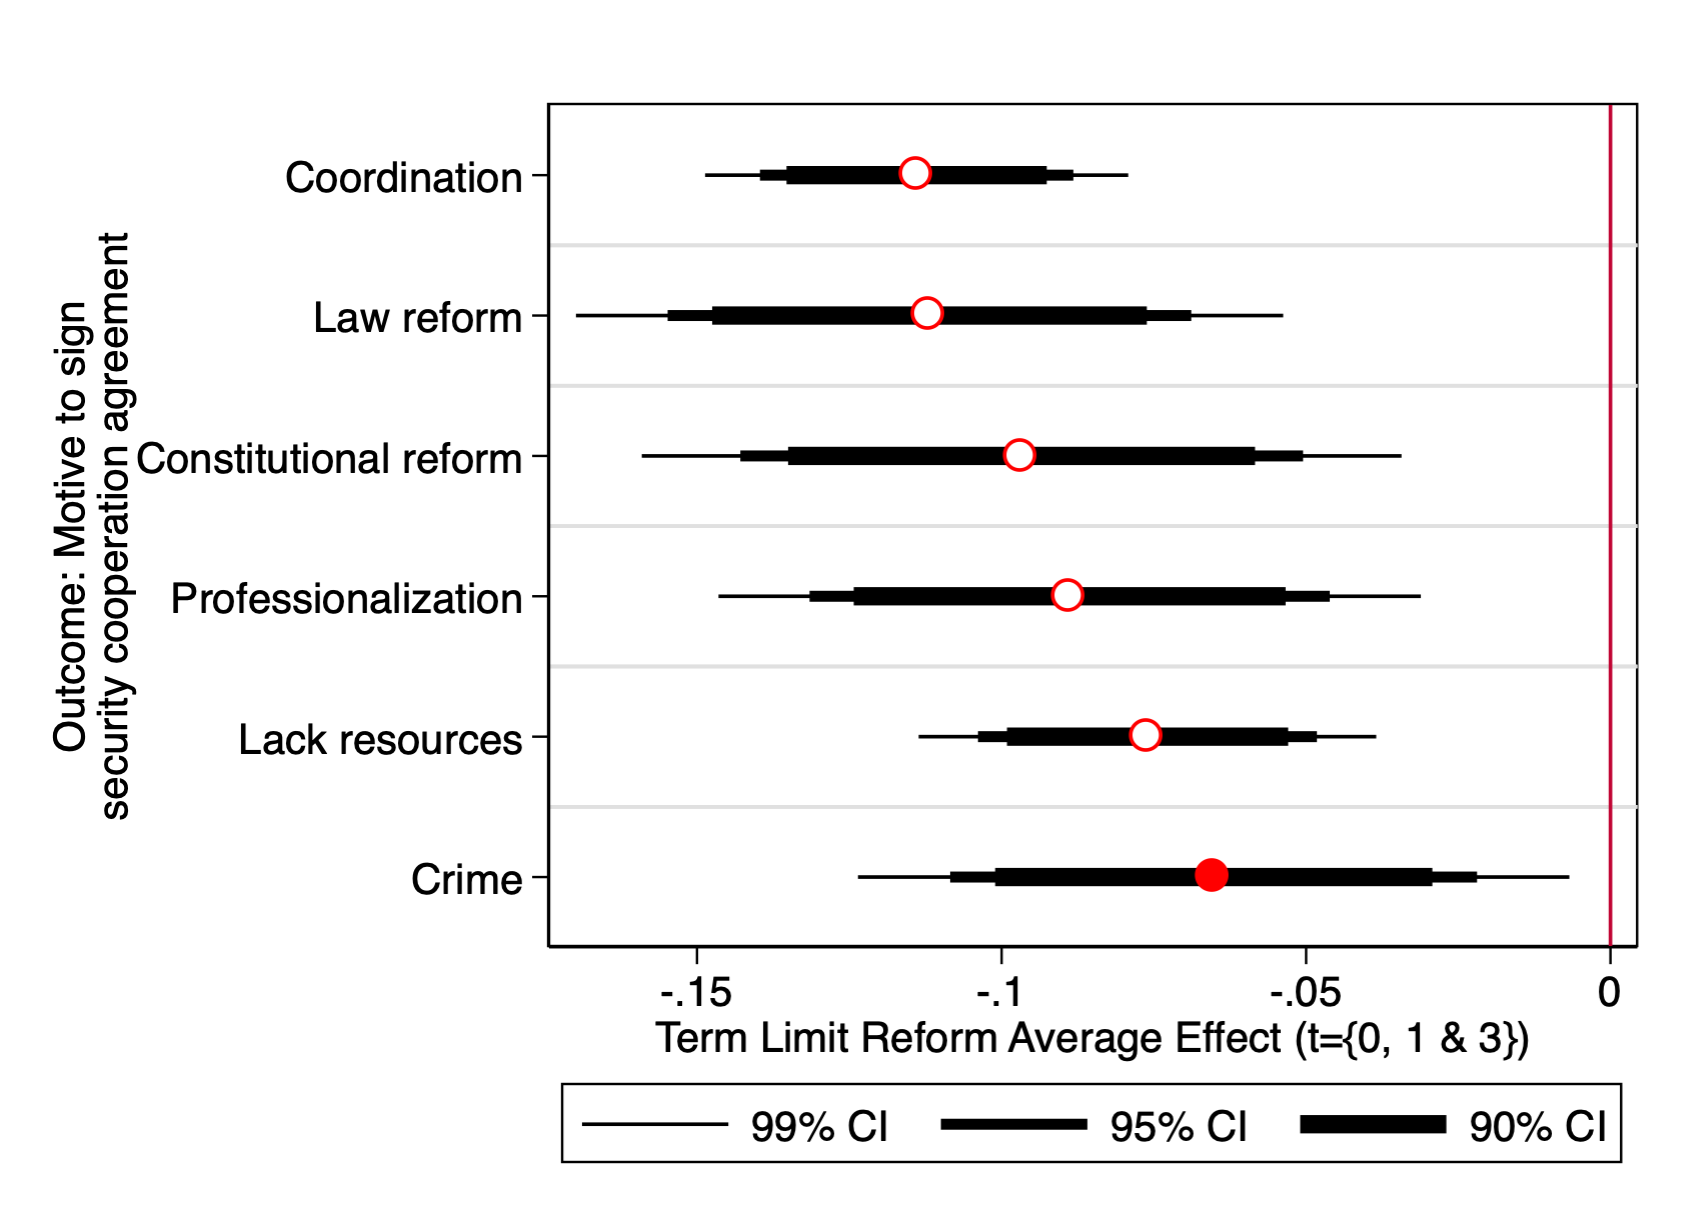
\includegraphics[width=0.9\textwidth]{Figures/motives.png}
       \captionsetup{justification=centering}
\end{figure}   

  \begin{landscape}
\begin{table}[htbp]\def\sym#1{\ifmmode^{#1}\else\(^{#1}\)\fi}
\centering
\caption{Effect of 2014 Term Limit Reform on Motives to Sign Security Agreements w/ Governor}
\label{tab:motives_final}
\scalebox{0.70}{
\begin{tabular}{lcccccc}
\hline \hline
\\ \multicolumn{7}{l}{Dependent variable:}\\
Motive: & Cons. reform  & Law reform & Lack resources & Professionalization & Coordination & Crime \\
& \multicolumn{1}{c}{(1)} & \multicolumn{1}{c}{(2)} & \multicolumn{1}{c}{(3)} & \multicolumn{1}{c}{(4)} & \multicolumn{1}{c}{(5)} & \multicolumn{1}{c}{(6)}  \\
\cmidrule(lrr){2-2}  \cmidrule(lrr){3-3} \cmidrule(lrr){4-4} \cmidrule(lrr){5-5} \cmidrule(lrr){6-6} \cmidrule(lrr){7-7} \\
\addlinespace
t-7 &     $ -0.2350^{***} $ &     $ -0.2581^{**} $ & $ -0.0955^{*} $ & $ -0.2000^{***} $  &     $ -0.1570^{*} $   &     $ -0.1538^{} $ \\
&     ($0.0407$) &     ($0.1175$) & ($0.0484$)& ($ 0.0671$)  &    ($0.0844$)   &   ($0.1078$) \\
t-6 &     $ -0.0758^{***} $ &     $ -0.0876^{***} $ &  $ -0.0615^{***} $ &  $ -0.0647^{} $  &     $ -0.0827^{**} $ &     $ -0.0369^{} $ \\
&     ($0.0176$) &     ($0.0199$) & ($0.0162$)& ($ 0.0585$)  &    ($0.0346$)   &   ($0.0265$) \\
t-5 &     $ 0.0223^{} $ &     $ -0.0405^{} $ &  $ 0.0574^{} $ &  $ 0.0580^{} $ &     $ -0.0106^{} $  &     $ 0.0427^{} $ \\
&     ($0.0591$) &     ($0.0583$) & ($0.0481$)& ($ 0.0750$)  &    ($0.0709$)   &   ($0.0445$) \\
t-4 &     $ 0.0167^{} $ &     $ -0.0832^{} $ &   $ 0.1207^{} $ &   $ 0.0649^{} $  &     $ -0.1313^{} $ &     $ 0.0346^{} $ \\
&     ($0.0987$) &     ($0.0842$) & ($0.0854$)& ($ 0.1053$)  &    ($0.2085$)   &   ($0.1173$) \\
t-3 &     $ -0.0385^{} $ &     $ -0.0160^{} $ &   $ 0.0727^{} $ &   $ 0.0802^{} $  &     $ 0.0403^{} $ &     $ 0.0734^{} $ \\
&     ($0.1052$) &     ($0.0840$) & ($0.1002$)& ($ 0.0738$)  &    ($0.1662$)   &   ($0.1061$) \\
t-2 &     $ -0.1162^{} $ &     $ -0.0914^{} $ &  $ 0.0228^{} $  &  $ -0.0822^{} $  &     $ -0.2796^{*} $ &     $ -0.0753^{} $ \\
&     ($0.1012$) &     ($0.0917$) & ($0.0640$)& ($ 0.1195$)  &    ($0.1379$)   &   ($0.0667$) \\
Reform (t=0) &     $ 0.0457^{} $ &     $ 0.0292^{} $ &   $ 0.0214^{} $   &   $ 0.0282^{} $  &     $ 0.0233^{} $ &     $ 0.0272^{*} $ \\
&     ($0.0278$) &     ($0.0183$) & ($0.0179$)& ($ 0.0201$)  &    ($0.0209$)   &   ($0.0146$) \\
t+1 &     $ -0.0906^{***} $ &     $ -0.1071^{***} $ &    $ -0.0935^{***} $ &    $ -0.0935^{***} $ &     $ -0.1215^{***} $ &     $ -0.0735^{***} $  \\
&     ($0.0164$) &     ($0.0182$) & ($0.0106$)& ($ 0.0160$)  &    ($0.0291$)   &   ($0.0121$) \\
t+3 &     $ -0.2452^{***} $ &     $ -0.2576^{***} $ &   $ -0.1560^{***} $  &   $ -0.2011^{***} $ &     $ -0.2436^{***} $ &     $ -0.1492^{***} $ \\
&     ($0.0535$) &     ($0.0484$) & ($0.0350$)& ($ 0.0463$)  &    ($0.0431$)   &   ($0.0527$) \\
\\
\addlinespace
Observations       &              9,725    &              9,725    &           9,725      &           9,725  &              9,725    &              9,725     \\
R-squared        &          0.2974 &          0.3021    &    0.2617       &           0.2722 &          0.2865 &          0.2594      \\
Mun. FEs      &     \checkmark         &  \checkmark   &     \checkmark         &  \checkmark  &     \checkmark         &  \checkmark   &     \checkmark         &  \checkmark   \\
Year. FEs    &     \checkmark         &  \checkmark   &     \checkmark         &  \checkmark &     \checkmark         &  \checkmark   &     \checkmark         &  \checkmark   \\
Controls$^b$  &    \checkmark     &       \checkmark  &    \checkmark      &   \checkmark &    \checkmark     &       \checkmark  &    \checkmark      &   \checkmark     \\
Cohort weighted  &   \checkmark      &       \checkmark  &   \checkmark       &   \checkmark  &   \checkmark      &       \checkmark  &   \checkmark       &   \checkmark    \\
Reform aggregate effect         & $-0.0967^{***} $$      & $-0.1118^{***} $$    & $-0.0760^{***} $$      & $-0.0888^{***} $$     & $-0.1139^{***} $$      & $-0.0652^{***} $$     \\
SE       & (0.0225)  & (0.0210) & (0.0136)  & (0.0208)  & (0.0125)  & (0.0211)   \\
\hline \hline
\multicolumn{7}{p{1.2\textwidth}}{\footnotesize{Notes: Coefficients show IW estimators following \citet{abraham_sun_2020}. Two relative time periods (lag 8 and 1) are removed to avoid collinearity problems noted by \citet{abraham_sun_2020}. Standard errors in parentheses are clustered at the state level for estimates in saturaded model. Significance-level: $^{***}$ 1\%; $^{**}$ 5\%; and $^*$ 10\%, that refer to two-sided t-test with the null hypothesis equal to 0 for each relative time period. $^a$ Even columns with outcomes with missing values where replaced by zeros assuming no activity was registered. $^b$ State-level controls include governor winning margin in last pre-treatment election and an indicator of whether the governor's party is the same as the federal incumbent party.}} \\
\end{tabular}
}
\end{table}
\end{landscape}
   

   %\begin{landscape}
\begin{table}[htbp]\def\sym#1{\ifmmode^{#1}\else\(^{#1}\)\fi}
\centering
\caption{Effect of 2014 Term Limit Reform on Motives to Sign Security Agreements w/ Governor}
\label{tab:motives_average_final}
\scalebox{0.70}{
\begin{tabular}{lcccccc}
\hline \hline
\\ \multicolumn{7}{l}{Dependent variable:}\\
Motive: & Cons. reform  & Law reform & Lack resources & Professionalization & Coordination & Crime \\
& \multicolumn{1}{c}{(1)} & \multicolumn{1}{c}{(2)} & \multicolumn{1}{c}{(3)} & \multicolumn{1}{c}{(4)} & \multicolumn{1}{c}{(5)} & \multicolumn{1}{c}{(6)}  \\
\cmidrule(lrr){2-2}  \cmidrule(lrr){3-3} \cmidrule(lrr){4-4} \cmidrule(lrr){5-5} \cmidrule(lrr){6-6} \cmidrule(lrr){7-7} \\
\addlinespace
Reform average effect         & $-0.0967^{***} $$      & $-0.1118^{***} $$     & $-0.0760^{***} $$        & $-0.0888^{***} $$       & $-0.1139^{***} $$        & $-0.0652^{***} $$       \\
& (0.0225)  & (0.0210) & (0.0136)  & (0.0208)  & (0.0125)  & (0.0211)   \\
\\
\addlinespace
Observations       &              9,725    &              9,725    &           9,725      &           9,725  &              9,725    &              9,725    \\
R-squared        &          0.2974 &          0.3021    &    0.2617       &           0.2722 &          0.2865 &          0.2594   \\
Mun. FEs      &     \checkmark         &  \checkmark   &     \checkmark         &  \checkmark  &     \checkmark         &  \checkmark   &     \checkmark         &  \checkmark   \\
Year. FEs    &     \checkmark         &  \checkmark   &     \checkmark         &  \checkmark &     \checkmark         &  \checkmark   &     \checkmark         &  \checkmark   \\
Controls$^b$  &    \checkmark     &       \checkmark  &    \checkmark      &   \checkmark &    \checkmark     &       \checkmark  &    \checkmark      &   \checkmark     \\
Cohort weighted  &   \checkmark      &       \checkmark  &   \checkmark       &   \checkmark  &   \checkmark      &       \checkmark  &   \checkmark       &   \checkmark    \\
Parallel trend holds &   \checkmark      &       \checkmark  &   \checkmark       &   \checkmark  &   \checkmark      &       \checkmark  &   \checkmark       &   \checkmark    \\
\hline \hline
\multicolumn{7}{p{1.2\textwidth}}{\footnotesize{Notes: Coefficients show IW estimators following \citet{abraham_sun_2020}. Two relative time periods (lag 8 and 1) are removed to avoid collinearity problems noted by \citet{abraham_sun_2020}. Standard errors in parentheses are clustered at the state level for estimates in saturaded model. Significance-level: $^{***}$ 1\%; $^{**}$ 5\%; and $^*$ 10\%, that refer to two-sided t-test with the null hypothesis equal to 0 for each relative time period. $^a$ Even columns with outcomes with missing values where replaced by zeros assuming no activity was registered. $^b$ State-level controls include governor winning margin in last pre-treatment election and an indicator of whether the governor's party is the same as the federal incumbent party.}} \\
\end{tabular}
}
\end{table}
\end{landscape}
  
   
   
      
\begin{landscape}
\begin{table}[htbp]\def\sym#1{\ifmmode^{#1}\else\(^{#1}\)\fi}
\centering
\caption{Effect of 2014 Term Limit Reform on Services Delegated to the Governor}
\label{tab:services}
\scalebox{0.70}{
\begin{tabular}{lcccccccc}
\hline \hline
\\ \multicolumn{9}{l}{Dependent variable:}\\
Service delegated: & Public security  & Traffic & Prevention & Training  & Technology & Research & Inteligence & Unify procedures \\
& \multicolumn{1}{c}{(1)} & \multicolumn{1}{c}{(2)} & \multicolumn{1}{c}{(3)} & \multicolumn{1}{c}{(4)} & \multicolumn{1}{c}{(5)} & \multicolumn{1}{c}{(6)} & \multicolumn{1}{c}{(7)} & \multicolumn{1}{c}{(8)} \\
\cmidrule(lrr){2-2}  \cmidrule(lrr){3-3} \cmidrule(lrr){4-4} \cmidrule(lrr){5-5} \cmidrule(lrr){6-6} \cmidrule(lrr){7-7} \cmidrule(lrr){8-8} \cmidrule(lrr){9-9} \\
\addlinespace
t-2 &     $ -0.0244^{} $ &     $ -0.0441^{} $ &  $ -0.0598^{***} $  &  $ -0.0565^{***} $  &     $ -0.0567^{***} $ &     $ -0.0596^{***} $ & $ -0.0596^{***} $ & $ -0.0506^{***} $   \\
&     ($0.1046$) &     ($0.0818$) & ($0.0021$)& ($ 0.0012$)  &    ($0.0016$)   &   ($0.0017$) \\
Reform (t=0) &     $ 0.0702^{} $ &     $ 0.0256^{} $ &   $ 0.0175^{} $   &   $ 0.0214^{} $  &     $ 0.0194^{} $ &     $ 0.0194^{} $ & $ 0.0204^{} $ & $ 0.0233^{} $   \\
&     ($0.0436$) &     ($0.0369$) & ($0.0137$)& ($ 0.0142$)  &    ($0.0126$)   &   ($0.0138$) \\
t+1 &     $ -0.0947^{*} $ &     $ -0.0259^{*} $ &    $ 0.0106^{} $ &    $ 0.0053^{} $ &     $ 0.0047^{} $ &     $ 0.0024^{} $  & $ 0.0018^{} $ & $ 0.0053^{} $   \\
&     ($0.0509$) &     ($0.0147$) & ($0.0198$)& ($ 0.0193$)  &    ($0.0197$)   &   ($0.0201$) \\
t+3 &     $ -0.2847^{***} $ &     $ 0.0000^{} $  \\
&     ($0.0430$) &     ($0.0000$)  \\
\\
\addlinespace
Observations       &              4,865    &              4,865    &           3,244      &           3,244  &              3,244    &              3,244  &              3,244    &              6,481   \\
R-squared        &          0.4234 &          0.3703    &    0.5567       &           0.5477 &          0.5409 &          0.5473     &        0.5467    &        0.4894   \\
Mun. FEs      &     \checkmark         &  \checkmark   &     \checkmark         &  \checkmark  &     \checkmark         &  \checkmark   &     \checkmark         &  \checkmark   \\
Year. FEs    &     \checkmark         &  \checkmark   &     \checkmark         &  \checkmark &     \checkmark         &  \checkmark   &     \checkmark         &  \checkmark   \\
Controls$^b$  &    \checkmark     &       \checkmark  &    \checkmark      &   \checkmark &    \checkmark     &       \checkmark  &    \checkmark      &   \checkmark     \\
Cohort weighted  &   \checkmark      &       \checkmark  &   \checkmark       &   \checkmark  &   \checkmark      &       \checkmark  &   \checkmark       &   \checkmark    \\
Reform average effect         & $-0.1031^{***} $$      & $-0.0242^{} $$     & $0.0094^{} $$        & $0.0133^{} $$       & $0.0121^{} $$        & $0.0109^{} $$    & $0.0111^{} $$      & $0.0143^{} $$     \\
SE (average effect)      & (0.0225)  & (0.0162) & (0.0080)  & (0.0120)  & (0.0117)  & (0.0122)    & (0.0123)  & (0.0114)   \\
\hline \hline
\multicolumn{9}{p{1.5\textwidth}}{\footnotesize{Notes: Coefficients show IW estimators following \citet{abraham_sun_2020}. Two relative time periods (lag 8 and 1) are removed to avoid collinearity problems noted by \citet{abraham_sun_2020}. Standard errors in parentheses are clustered at the state level for estimates in saturaded model. Significance-level: $^{***}$ 1\%; $^{**}$ 5\%; and $^*$ 10\%, that refer to two-sided t-test with the null hypothesis equal to 0 for each relative time period. $^a$ Even columns with outcomes with missing values where replaced by zeros assuming no activity was registered. $^b$ State-level controls include governor winning margin in last pre-treatment election and an indicator of whether the governor's party is the same as the federal incumbent party.}} \\
\end{tabular}
}
\end{table}
\end{landscape}
   
%\begin{landscape}
\begin{table}[htbp]\def\sym#1{\ifmmode^{#1}\else\(^{#1}\)\fi}
\centering
\caption{Effect of 2014 Term Limit Reform on Services Delegated to the Governor}
\label{tab:services_average}
\scalebox{0.70}{
\begin{tabular}{lcccccccc}
\hline \hline
\\ \multicolumn{9}{l}{Dependent variable:}\\
Service delegated: & Public security  & Traffic & Prevention & Training  & Technology & Research & Inteligence & Unify procedures \\
& \multicolumn{1}{c}{(1)} & \multicolumn{1}{c}{(2)} & \multicolumn{1}{c}{(3)} & \multicolumn{1}{c}{(4)} & \multicolumn{1}{c}{(5)} & \multicolumn{1}{c}{(6)} & \multicolumn{1}{c}{(7)} & \multicolumn{1}{c}{(8)} \\
\cmidrule(lrr){2-2}  \cmidrule(lrr){3-3} \cmidrule(lrr){4-4} \cmidrule(lrr){5-5} \cmidrule(lrr){6-6} \cmidrule(lrr){7-7} \cmidrule(lrr){8-8} \cmidrule(lrr){9-9} \\
\addlinespace
Reform average effect         & $0.0149^{*} $$      & $0.0579^{***} $$     & $0.0426^{***} $$        & $0.0034^{} $$       & $-0.0345^{***} $$        & $-0.0819^{***} $$    & $0.0092^{} $$      & $0.0056^{} $$     \\
SE       & (0.0079)  & (0.0099) & (0.0046)  & (0.0048)  & (0.0103)  & (0.0085)    & (0.0063)  & (0.0034)   \\
\addlinespace
Observations       &             11,353    &             11,353    &          11,353      &          11,353  &             11,353    &             11,353  &             11,353    &             11,353   \\
R-squared        &          0.8662 &          0.8556    &    0.9239       &           0.8767 &          0.8548 &          0.8954     &        0.8557    &        0.7008   \\
Mun. FEs      &     \checkmark         &  \checkmark   &     \checkmark         &  \checkmark  &     \checkmark         &  \checkmark   &     \checkmark         &  \checkmark   \\
Year. FEs    &     \checkmark         &  \checkmark   &     \checkmark         &  \checkmark &     \checkmark         &  \checkmark   &     \checkmark         &  \checkmark   \\
Controls$^b$  &    \checkmark     &       \checkmark  &    \checkmark      &   \checkmark &    \checkmark     &       \checkmark  &    \checkmark      &   \checkmark     \\
Cohort weighted  &   \checkmark      &       \checkmark  &   \checkmark       &   \checkmark  &   \checkmark      &       \checkmark  &   \checkmark       &   \checkmark    \\
Parallel trend holds &   \checkmark      &       \checkmark  &          &     &         &       &          &       \\
\hline \hline
\multicolumn{9}{p{1.5\textwidth}}{\footnotesize{Notes: Coefficients show IW estimators following \citet{abraham_sun_2020}. Two relative time periods (lag 8 and 1) are removed to avoid collinearity problems noted by \citet{abraham_sun_2020}. Standard errors in parentheses are clustered at the state level for estimates in saturaded model. Significance-level: $^{***}$ 1\%; $^{**}$ 5\%; and $^*$ 10\%, that refer to two-sided t-test with the null hypothesis equal to 0 for each relative time period. $^a$ Even columns with outcomes with missing values where replaced by zeros assuming no activity was registered. $^b$ State-level controls include governor winning margin in last pre-treatment election and an indicator of whether the governor's party is the same as the federal incumbent party.}} \\
\end{tabular}
}
\end{table}
\end{landscape}
   

\begin{landscape}
\begin{table}[htbp]\def\sym#1{\ifmmode^{#1}\else\(^{#1}\)\fi}
\centering
\caption{Effect of 2014 Term Limit Reform on Services Delegated to the Governor}
\label{tab:interaction_alignment}
\scalebox{0.70}{
\begin{tabular}{lccc}
\hline \hline
\\ \multicolumn{4}{l}{Dependent variable: Signing Security Cooperation Agreement w/ Governor}\\
Alignment: & w/ President  & w/ Governor  & w/ Governor from PRI \\
& \multicolumn{1}{c}{(1)} & \multicolumn{1}{c}{(2)} & \multicolumn{1}{c}{(3)} \\
\cmidrule(lrr){2-2}  \cmidrule(lrr){3-3} \cmidrule(lrr){4-4} \\
\addlinespace
t-7 &     $ -0.2383^{*} $ &     $ -0.0191^{*} $ &  $ 0.0000^{} $ \\
&     ($0.1348$) &     ($0.0108$) & ($0.0000$) \\
t-6 &     $ -0.0807^{} $ &     $ 0.0199^{} $ &  $ -0.0430^{} $  \\
&     ($0.0873$) &     ($0.0499$) & ($0.0467$) \\
t-5 &     $ -0.1186^{} $ &     $ -0.2028^{**} $ &  $ -0.2406^{**} $  \\
&     ($0.1046$) &     ($0.0924$) & ($0.0922$) \\
t-4 &     $ 0.0665^{} $ &     $ -0.0784^{} $ &  $ -0.1077^{} $  \\
&     ($0.1483$) &     ($0.1203$) & ($0.1236$) \\
t-3 &     $ 0.3395^{**} $ &     $ 0.2569^{***} $ &  $ 0.2303^{***} $  \\
&     ($0.1651$) &     ($0.0720$) & ($0.0702$) \\
t-2 &     $ 0.0027^{} $ &     $ -0.0253^{} $ &  $ 0.0976^{} $  \\
&     ($0.1572$) &     ($0.1182$) & ($0.1471$) \\
Reform (t=0) &     $ -0.1686^{} $ &     $ -0.2236^{} $ &   $ 0.1790^{} $   \\
&     ($0.1877$) &     ($0.1316$) & ($0.1258$) \\
t+1 &     $ -0.2169^{} $ &     $ -0.5692^{**} $ &    $ -0.0199^{} $ \\
&     ($0.1884$) &     ($0.2119$) & ($0.1549$) \\
t+2 &     $ -0.1125^{} $ &     $ -0.5020^{*} $  &     $ -0.4753^{*} $ \\
&     ($0.2496$) &     ($0.2690$)  & ($0.2741$) \\
t+3 &     $ -0.2197^{} $ &     $ -0.3562^{} $  &     $ -0.3876^{} $ \\
&     ($0.2241$) &     ($0.3827$)  & ($0.3818$) \\
\\
\addlinespace
Observations       &             12,173    &             12,173    &          12,173    \\
R-squared        &          0.4555 &          0.4566    &    0.4541    \\
Mun. FEs      &     \checkmark         &  \checkmark   &     \checkmark    \\
Year. FEs    &     \checkmark         &  \checkmark   &     \checkmark    \\
Controls$^b$  &    \checkmark     &       \checkmark  &    \checkmark   \\
Cohort weighted  &   \checkmark      &       \checkmark  &   \checkmark    \\
Reform average effect         & $-0.1376^{} $$      & $-0.1538^{*} $$     & $-0.0551^{} $$     \\
SE (average effect)      & (0.1313)  & (0.0906) & (0.0652) \\
\hline \hline
\multicolumn{4}{p{1.5\textwidth}}{\footnotesize{Notes: Coefficients show IW estimators following \citet{abraham_sun_2020}. Two relative time periods (lag 8 and 1) are removed to avoid collinearity problems noted by \citet{abraham_sun_2020}. Standard errors in parentheses are clustered at the state level for estimates in saturaded model. Significance-level: $^{***}$ 1\%; $^{**}$ 5\%; and $^*$ 10\%, that refer to two-sided t-test with the null hypothesis equal to 0 for each relative time period. $^a$ Even columns with outcomes with missing values where replaced by zeros assuming no activity was registered. $^b$ State-level controls include governor winning margin in last pre-treatment election and an indicator of whether the governor's party is the same as the federal incumbent party.}} \\
\end{tabular}
}
\end{table}
\end{landscape}
   
%\begin{landscape}
\begin{table}[htbp]\def\sym#1{\ifmmode^{#1}\else\(^{#1}\)\fi}
\centering
\caption{Effect of 2014 Term Limit Reform on Services Delegated to the Governor}
\label{tab:interaction_alignment_average}
\scalebox{0.70}{
\begin{tabular}{lccc}
\hline \hline
\\ \multicolumn{4}{l}{Dependent variable: Signing Security Cooperation Agreement w/ Governor}\\
Alignment: & w/ President  & w/ Governor  & w/ Governor from PRI \\
& \multicolumn{1}{c}{(1)} & \multicolumn{1}{c}{(2)} & \multicolumn{1}{c}{(3)} \\
\cmidrule(lrr){2-2}  \cmidrule(lrr){3-3} \cmidrule(lrr){4-4} \\
\addlinespace
Reform average effect         & $-0.1376^{} $$      & $-0.1538^{*} $$     & $-0.0551^{} $$     \\
& (0.1313)  & (0.0906) & (0.0652) \\
\\
\addlinespace
Observations       &             12,173    &             12,173    &          12,173    \\
R-squared        &          0.4555 &          0.4566    &    0.4541    \\
Mun. FEs      &     \checkmark         &  \checkmark   &     \checkmark    \\
Year. FEs    &     \checkmark         &  \checkmark   &     \checkmark    \\
Controls$^b$  &    \checkmark     &       \checkmark  &    \checkmark   \\
Cohort weighted  &   \checkmark      &       \checkmark  &   \checkmark    \\
\hline \hline
\multicolumn{4}{p{1.5\textwidth}}{\footnotesize{Notes: Coefficients show IW estimators following \citet{abraham_sun_2020}. Two relative time periods (lag 8 and 1) are removed to avoid collinearity problems noted by \citet{abraham_sun_2020}. Standard errors in parentheses are clustered at the state level for estimates in saturaded model. Significance-level: $^{***}$ 1\%; $^{**}$ 5\%; and $^*$ 10\%, that refer to two-sided t-test with the null hypothesis equal to 0 for each relative time period. $^a$ Even columns with outcomes with missing values where replaced by zeros assuming no activity was registered. $^b$ State-level controls include governor winning margin in last pre-treatment election and an indicator of whether the governor's party is the same as the federal incumbent party.}} \\
\end{tabular}
}
\end{table}
\end{landscape}
   

              
\begin{landscape}
\begin{table}[htbp]\def\sym#1{\ifmmode^{#1}\else\(^{#1}\)\fi}
\centering
\caption{Effect of 2014 Term Limit Reform on Services Delegated to the Governor}
\label{tab:interaction_trust}
\scalebox{0.70}{
\begin{tabular}{lcccccccc}
\hline \hline
\\ \multicolumn{9}{l}{Dependent variable: Signing Security Cooperation Agreement w/ Governor}\\
Jurisdiction: & \multicolumn{2}{c}{Municipal} & \multicolumn{2}{c}{State} & \multicolumn{4}{c}{Federal} \\
Police force: & Traffic  & Preventive  & State Police & State Attorney Police & Federal Police & Ministerial Police & Army & Marines \\
& \multicolumn{1}{c}{(1)} & \multicolumn{1}{c}{(2)} & \multicolumn{1}{c}{(3)} & \multicolumn{1}{c}{(4)} & \multicolumn{1}{c}{(5)} & \multicolumn{1}{c}{(6)} & \multicolumn{1}{c}{(7)} & \multicolumn{1}{c}{(8)} \\
\cmidrule(lrr){2-2}  \cmidrule(lrr){3-3} \cmidrule(lrr){4-4} \cmidrule(lrr){5-5} \cmidrule(lrr){6-6} \cmidrule(lrr){7-7} \cmidrule(lrr){8-8} \cmidrule(lrr){9-9} \\
\addlinespace
t-7 &     $ 0.1781^{} $ &     $ 0.0000^{} $ &  $ 0.1737^{} $  &  $ 0.1270^{} $  &     $ 0.0908^{} $ &     $ 0.1162^{} $ & $ 0.1093^{*} $ & $ 0.0788^{} $   \\
&     ($0.1657$) &     ($0.0000$) & ($0.1372$)& ($ 0.1137$)  &    ($0.0736$)   &   ($0.0858$) \\
t-6 &     $ -0.0459^{} $ &     $ -0.0601^{} $ &  $ -0.0414^{} $  &  $ -0.0565^{} $  &     $ 0.0055^{} $ &     $ -0.0537^{} $ & $ 0.0234^{} $ & $ 0.0038^{} $   \\
&     ($0.0801$) &     ($0.0481$) & ($0.0539$)& ($ 0.0457$)  &    ($0.0390$)   &   ($0.0379$) \\
t-5 &     $ -0.8924^{***} $ &     $ -0.2958^{} $ &  $ -0.7754^{} $  &  $ -1.3246^{} $  &     $ -0.8583^{**} $ &     $ -1.3844^{***} $ & $ -0.6699^{**} $ & $ -0.5789^{} $   \\
&     ($0.2538$) &     ($0.2470$) & ($0.6291$)& ($ 0.9127$)  &    ($0.3310$)   &   ($0.2853$) \\
t-4 &     $ -0.8387^{} $ &     $ -0.4847^{} $ &  $ -0.8341^{} $  &  $ -1.8134^{} $  &     $ -1.0918^{} $ &     $ -1.2394^{} $ & $ -0.3796^{} $ & $ -0.4926^{} $   \\
&     ($0.7688$) &     ($0.7827$) & ($0.7594$)& ($ 1.3210$)  &    ($0.7492$)   &   ($1.0419$) \\
t-3 &     $ -0.0581^{} $ &     $ -0.2251^{} $ &  $ -0.4852^{} $  &  $ -1.8471^{} $  &     $ -0.6960^{} $ &     $ -0.8290^{} $ & $ 0.1192^{} $ & $ -0.1124^{} $   \\
&     ($0.8135$) &     ($0.8597$) & ($0.7511$)& ($ 1.3390$)  &    ($0.8562$)   &   ($1.1144$) \\
t-2 &     $ 0.0341^{} $ &     $ -0.2671^{} $ &  $ -0.2891^{} $  &  $ -0.6196^{} $  &     $ -0.6138^{} $ &     $ -0.3468^{} $ & $ -0.4246^{} $ & $ -0.4023^{} $   \\
&     ($0.5384$) &     ($0.5922$) & ($0.4176$)& ($ 0.8966$)  &    ($0.4795$)   &   ($0.7851$) \\
Reform (t=0) &     $ -0.4444^{} $ &     $ 0.1161^{} $ &   $ -0.5432^{} $   &   $ -0.3590^{} $  &     $ -1.2942^{**} $ &     $ -0.8581^{} $ & $ -0.4514^{} $ & $ -0.8446^{} $   \\
&     ($0.4490$) &     ($0.4975$) & ($0.4116$)& ($ 1.1629$)  &    ($0.5674$)   &   ($0.7678$) \\
t+1 &     $ -0.9836^{} $ &     $ -0.2186^{} $ &    $ -1.3877^{**} $ &    $ -1.3449^{} $ &     $ -2.4941^{***} $ &     $ -1.8551^{*} $  & $ -1.5407^{**} $ & $ -1.8918^{**} $   \\
&     ($0.5947$) &     ($0.5769$) & ($0.6053$)& ($ 1.4393$)  &    ($0.7475$)   &   ($0.9449$) \\
t+2 &     $ -1.8506^{***} $ &     $ -1.6311^{**} $  \\
&     ($0.5938$) &     ($0.6871$)  \\
t+3 &     $ -0.1376^{} $ &     $ -1.5275^{} $  \\
&     ($1.1164$) &     ($1.1456$)  \\
\\
\addlinespace
Observations       &             12,173    &             12,173    &          12,173      &          12,173  &             12,173    &             12,173  &             12,173    &             12,173   \\
R-squared        &          0.4666 &          0.4641    &    0.4675       &           0.4673 &          0.4642 &          0.4719     &        0.4666    &        0.4666   \\
Mun. FEs      &     \checkmark         &  \checkmark   &     \checkmark         &  \checkmark  &     \checkmark         &  \checkmark   &     \checkmark         &  \checkmark   \\
Year. FEs    &     \checkmark         &  \checkmark   &     \checkmark         &  \checkmark &     \checkmark         &  \checkmark   &     \checkmark         &  \checkmark   \\
Controls$^b$  &    \checkmark     &       \checkmark  &    \checkmark      &   \checkmark &    \checkmark     &       \checkmark  &    \checkmark      &   \checkmark     \\
Cohort weighted  &   \checkmark      &       \checkmark  &   \checkmark       &   \checkmark  &   \checkmark      &       \checkmark  &   \checkmark       &   \checkmark    \\
Reform average effect         & $-0.1399^{} $$      & $-0.2053^{} $$     & $-0.3431^{**} $$        & $-0.2984^{**} $$       & $-0.5738^{**} $$        & $-0.2614^{**} $$    & $-0.4633^{} $$      & $-0.4835^{*} $$     \\
SE (average effect)      & (0.0944)  & (0.1633) & (0.1594)  & (0.1455)  & (0.2673)  & (0.1107)    & (0.4247)  & (0.2373)   \\
\hline \hline
\multicolumn{9}{p{1.5\textwidth}}{\footnotesize{Notes: Coefficients show IW estimators following \citet{abraham_sun_2020}. Two relative time periods (lag 8 and 1) are removed to avoid collinearity problems noted by \citet{abraham_sun_2020}. Standard errors in parentheses are clustered at the state level for estimates in saturaded model. Significance-level: $^{***}$ 1\%; $^{**}$ 5\%; and $^*$ 10\%, that refer to two-sided t-test with the null hypothesis equal to 0 for each relative time period. $^a$ Even columns with outcomes with missing values where replaced by zeros assuming no activity was registered. $^b$ State-level controls include governor winning margin in last pre-treatment election and an indicator of whether the governor's party is the same as the federal incumbent party.}} \\
\end{tabular}
}
\end{table}
\end{landscape}
   
%\begin{landscape}
\begin{table}[htbp]\def\sym#1{\ifmmode^{#1}\else\(^{#1}\)\fi}
\centering
\caption{Reform interaction with citizens' preferences}
\label{tab:interaction_trust_average}
\scalebox{0.70}{
\begin{tabular}{lcccccccc}
\hline \hline
\\ \multicolumn{9}{l}{Dependent variable: Signing Security Cooperation Agreement w/ Governor}\\
Jurisdiction: & \multicolumn{2}{c}{Municipal} & \multicolumn{2}{c}{State} & \multicolumn{4}{c}{Federal} \\
Trust in Police Force: & Traffic  & Preventive  & State Police & State Attorney Police & Federal Police & Ministerial Police & Army & Marines \\
& \multicolumn{1}{c}{(1)} & \multicolumn{1}{c}{(2)} & \multicolumn{1}{c}{(3)} & \multicolumn{1}{c}{(4)} & \multicolumn{1}{c}{(5)} & \multicolumn{1}{c}{(6)} & \multicolumn{1}{c}{(7)} & \multicolumn{1}{c}{(8)} \\
\cmidrule(lrr){2-2}  \cmidrule(lrr){3-3} \cmidrule(lrr){4-4} \cmidrule(lrr){5-5} \cmidrule(lrr){6-6} \cmidrule(lrr){7-7} \cmidrule(lrr){8-8} \cmidrule(lrr){9-9} \\
\addlinespace
Reform average effect         & $-0.1400^{} $$      & $-0.2053^{} $$     & $-0.3431^{**} $$        & $-0.2984^{**} $$       & $-0.5739^{**} $$        & $-0.2614^{**} $$    & $-0.4636^{} $$      & $-0.4837^{*} $$     \\
SE (average effect)      & (0.0944)  & (0.1633) & (0.1594)  & (0.1455)  & (0.2673)  & (0.1107)    & (0.4248)  & (0.2374)   \\
\\
\addlinespace
Observations       &             12,173    &             12,173    &          12,173      &          12,173  &             12,173    &             12,173  &             12,173    &             12,173   \\
R-squared        &          0.4666 &          0.4641    &    0.4675       &           0.4673 &          0.4642 &          0.4719     &        0.4666    &        0.4666   \\
Mun. FEs      &     \checkmark         &  \checkmark   &     \checkmark         &  \checkmark  &     \checkmark         &  \checkmark   &     \checkmark         &  \checkmark   \\
Year. FEs    &     \checkmark         &  \checkmark   &     \checkmark         &  \checkmark &     \checkmark         &  \checkmark   &     \checkmark         &  \checkmark   \\
Controls$^b$  &    \checkmark     &       \checkmark  &    \checkmark      &   \checkmark &    \checkmark     &       \checkmark  &    \checkmark      &   \checkmark     \\
Cohort weighted  &   \checkmark      &       \checkmark  &   \checkmark       &   \checkmark  &   \checkmark      &       \checkmark  &   \checkmark       &   \checkmark    \\
\hline \hline
\multicolumn{9}{p{1.5\textwidth}}{\footnotesize{Notes: Coefficients show IW estimators following \citet{abraham_sun_2020}. Two relative time periods (lag 8 and 1) are removed to avoid collinearity problems noted by \citet{abraham_sun_2020}. Standard errors in parentheses are clustered at the state level, with the following significance-level: $^{***}$ 1\%; $^{**}$ 5\%; and $^*$ 10\%, that refer to two-sided t-test with the null hypothesis equal to 0 for each relative time period. $^a$ Refers to security cooperation agreements signed with the Governor. $^b$ Pretreatment controls include: governor winning margin; party alignment with the President;  party alignment with the Governor; municipal winning margin; logged population; logged organized crime related deaths; and Cartel presence.}} \\
\end{tabular}
}
\end{table}
\end{landscape}
   
 
\begin{landscape}
\begin{table}[htbp]\def\sym#1{\ifmmode^{#1}\else\(^{#1}\)\fi}
\centering
\caption{Reform interaction with citizens' being able to identify a Police Force}
\label{tab:interaction_identify}
\scalebox{0.70}{
\begin{tabular}{lcccccccc}
\hline \hline
\\ \multicolumn{9}{l}{Dependent variable: Signing Security Cooperation Agreement w/ Governor}\\
Jurisdiction: & \multicolumn{2}{c}{Municipal} & \multicolumn{2}{c}{State} & \multicolumn{4}{c}{Federal} \\
Identify Policy Force: & Traffic  & Preventive  & State Police & State Attorney Police & Federal Police & Ministerial Police & Army & Marines \\
& \multicolumn{1}{c}{(1)} & \multicolumn{1}{c}{(2)} & \multicolumn{1}{c}{(3)} & \multicolumn{1}{c}{(4)} & \multicolumn{1}{c}{(5)} & \multicolumn{1}{c}{(6)} & \multicolumn{1}{c}{(7)} & \multicolumn{1}{c}{(8)} \\
\cmidrule(lrr){2-2}  \cmidrule(lrr){3-3} \cmidrule(lrr){4-4} \cmidrule(lrr){5-5} \cmidrule(lrr){6-6} \cmidrule(lrr){7-7} \cmidrule(lrr){8-8} \cmidrule(lrr){9-9} \\
\addlinespace
t-7 &     $ -0.8572^{} $ &     $ 0.1007^{} $ &  $ 0.0649^{} $  &  $ 0.0783^{} $  &     $ -2.5321^{***} $ &     $ 0.0632^{} $ & $ -1.4640^{*} $ & $ 0.0539^{} $   \\
&     ($0.6544$) &     ($0.0978$) & ($0.0611$)& ($ 0.0697$)  &    ($0.8962$)   &   ($0.0550$) &    ($0.8372$)   &   ($0.0455$) \\
t-6 &     $ -0.2641^{} $ &     $ 0.0248^{} $ &  $ 0.0135^{} $  &  $ 0.0056^{} $  &     $ -0.7692^{***} $ &     $ -0.0035^{} $ & $ -0.4466^{*} $ & $ 0.0092^{} $   \\
&     ($0.2039$) &     ($0.0609$) & ($0.0467$)& ($ 0.0441$)  &    ($0.2696$)   &   ($0.0413$) &    ($0.2577$)   &   ($0.0423$) \\
t-5 &     $ -0.4097^{} $ &     $ -0.0652^{} $ &  $ 0.6451^{} $  &  $ 0.1762^{} $  &     $ -1.1340^{**} $ &     $ -0.7691^{***} $ & $ -0.8805^{} $ & $ -0.3720^{} $   \\
&     ($0.3986$) &     ($0.3080$) & ($0.3960$)& ($ 0.4004$)  &    ($0.4306$)   &   ($0.2589$) &    ($0.5274$)   &   ($0.2421$) \\
t-4 &     $ 0.3350^{} $ &     $ 0.1050^{} $ &  $ 0.7461^{} $  &  $ -0.0893^{} $  &     $ -1.6040^{***} $ &     $ -0.2211^{} $ & $ -0.7589^{} $ & $ -0.3294^{} $   \\
&     ($0.5455$) &     ($0.5451$) & ($0.4774$)& ($ 0.6583$)  &    ($0.5716$)   &   ($0.7553$) &    ($0.8538$)   &   ($0.4995$) \\
t-3 &     $ 0.8549^{} $ &     $ 0.3354^{} $ &  $ 0.8618^{*} $  &  $ -0.1098^{} $  &     $ -1.2530^{**} $ &     $ 0.2973^{} $ & $ -0.3261^{} $ & $ -0.0407^{} $   \\
&     ($0.5572$) &     ($0.6384$) & ($0.5038$)& ($ 0.7313$)  &    ($0.6065$)   &   ($0.8187$) &    ($0.8829$)   &   ($0.5638$) \\
t-2 &     $ -0.0741^{} $ &     $ 0.0173^{} $ &  $ 0.3106^{} $  &  $ -0.0035^{} $  &     $ -1.1572^{**} $ &     $ -0.2290^{} $ & $ -0.7416^{} $ & $ -0.3552^{} $   \\
&     ($0.3985$) &     ($0.3426$) & ($0.3583$)& ($ 0.4741$)  &    ($0.4705$)   &   ($0.5458$) &    ($0.5501$)   &   ($0.3444$) \\
Reform (t=0) &     $ 0.0965^{} $ &     $ -0.3095^{} $ &   $ -0.6740^{} $   &   $ -0.0176^{} $  &     $ -1.7122^{***} $ &     $ -0.3017^{} $ & $ -0.8230^{} $ & $ -0.7614^{} $   \\
&     ($0.3746$) &     ($0.5580$) & ($0.5072$)& ($ 0.5448$)  &    ($0.5196$)   &   ($0.5185$) &    ($0.5125$)   &   ($0.4724$) \\
t+1 &     $ 0.1452^{} $ &     $ -0.8415^{} $ &    $ -0.5733^{} $ &    $ -0.5894^{} $ &     $ -1.1449^{**} $ &     $ -1.2316^{} $  & $ -0.8753^{} $ & $ -1.6442^{***} $   \\
&     ($0.4015$) &     ($0.7920$) & ($0.6386$)& ($ 0.7035$)  &    ($0.4877$)   &   ($0.7296$) &    ($0.5560$)   &   ($0.5433$) \\
t+2 &     $ 0.4499^{} $ &     $ -0.7212^{} $ &    $ 0.0862^{} $ &    $ -1.4956^{**} $ &     $ -0.5687^{} $ &     $ -1.6626^{**} $  & $ -0.4091^{} $ & $ -1.5000^{**} $   \\
&     ($0.3760$) &     ($0.7799$) & ($0.6272$)& ($ 0.7215$)  &    ($0.5955$)   &   ($0.6266$) &    ($0.6311$)   &   ($0.5652$) \\
t+3 &     $ 1.1277^{} $ &     $ -0.5739^{} $ &    $ -0.6702^{} $ &    $ -1.2519^{} $ &     $ -1.7933^{} $ &     $ 0.0623^{} $  & $ -0.5981^{} $ & $ -1.0885^{} $   \\
&     ($0.9218$) &     ($1.2931$) & ($0.9352$)& ($ 1.0598$)  &    ($1.0758$)   &   ($1.0916$) &    ($0.9325$)   &   ($0.9434$) \\
\\
\addlinespace
Observations       &             12,173    &             12,173    &          12,173      &          12,173  &             12,173    &             12,173  &             12,173    &             12,173   \\
R-squared        &          0.4688 &          0.4599    &    0.4659       &           0.4658 &          0.4624 &          0.4783     &        0.4645    &        0.4655   \\
Mun. FEs      &     \checkmark         &  \checkmark   &     \checkmark         &  \checkmark  &     \checkmark         &  \checkmark   &     \checkmark         &  \checkmark   \\
Year. FEs    &     \checkmark         &  \checkmark   &     \checkmark         &  \checkmark &     \checkmark         &  \checkmark   &     \checkmark         &  \checkmark   \\
Controls$^b$  &    \checkmark     &       \checkmark  &    \checkmark      &   \checkmark &    \checkmark     &       \checkmark  &    \checkmark      &   \checkmark     \\
Cohort weighted  &   \checkmark      &       \checkmark  &   \checkmark       &   \checkmark  &   \checkmark      &       \checkmark  &   \checkmark       &   \checkmark    \\
Reform average effect         & $0.3037^{} $      & $-0.4471^{} $     & $-0.2964^{} $        & $-0.3087^{} $       & $-0.7782^{**} $        & $-0.2768^{} $    & $-0.5017^{} $      & $-0.5781^{**} $     \\
SE (average effect)      & (0.3233)  & (0.6044) & (0.3716)  & (0.2401)  & (0.2868)  & (0.2411)    & (0.4665)  & (0.2669)   \\
\hline \hline
\multicolumn{9}{p{1.6\textwidth}}{\footnotesize{Notes: Coefficients show IW estimators following \citet{abraham_sun_2020}. Two relative time periods (lag 8 and 1) are removed to avoid collinearity problems noted by \citet{abraham_sun_2020}. Standard errors in parentheses are clustered at the state level, with the following significance-level: $^{***}$ 1\%; $^{**}$ 5\%; and $^*$ 10\%, that refer to two-sided t-test with the null hypothesis equal to 0 for each relative time period. $^a$ Refers to security cooperation agreements signed with the Governor. $^b$ Pretreatment controls include: governor winning margin; party alignment with the President;  party alignment with the Governor; municipal winning margin; logged population; logged organized crime related deaths; and Cartel presence.}} \\
\end{tabular}
}
\end{table}
\end{landscape}
   
%\begin{landscape}
\begin{table}[htbp]\def\sym#1{\ifmmode^{#1}\else\(^{#1}\)\fi}
\centering
\caption{Reform interaction with citizens' being able to identify a Police Force}
\label{tab:interaction_identify_average}
\scalebox{0.70}{
\begin{tabular}{lcccccccc}
\hline \hline
\\ \multicolumn{9}{l}{Dependent variable: Signing Security Cooperation Agreement w/ Governor}\\
Jurisdiction: & \multicolumn{2}{c}{Municipal} & \multicolumn{2}{c}{State} & \multicolumn{4}{c}{Federal} \\
Identify Policy Force: & Traffic  & Preventive  & State Police & State Attorney Police & Federal Police & Ministerial Police & Army & Marines \\
& \multicolumn{1}{c}{(1)} & \multicolumn{1}{c}{(2)} & \multicolumn{1}{c}{(3)} & \multicolumn{1}{c}{(4)} & \multicolumn{1}{c}{(5)} & \multicolumn{1}{c}{(6)} & \multicolumn{1}{c}{(7)} & \multicolumn{1}{c}{(8)} \\
\cmidrule(lrr){2-2}  \cmidrule(lrr){3-3} \cmidrule(lrr){4-4} \cmidrule(lrr){5-5} \cmidrule(lrr){6-6} \cmidrule(lrr){7-7} \cmidrule(lrr){8-8} \cmidrule(lrr){9-9} \\
\addlinespace
Reform average effect         & $0.3037^{} $$      & $-0.4471^{} $$     & $-0.2964^{} $$        & $-0.3087^{} $$       & $-0.7782^{**} $$        & $-0.2768^{} $$    & $-0.5017^{} $$      & $-0.5781^{**} $$     \\
SE (average effect)      & (0.3233)  & (0.6044) & (0.3716)  & (0.2401)  & (0.2868)  & (0.2411)    & (0.4665)  & (0.2669)   \\
\\
\addlinespace
Observations       &             12,173    &             12,173    &          12,173      &          12,173  &             12,173    &             12,173  &             12,173    &             12,173   \\
R-squared        &          0.4688 &          0.4599    &    0.4659       &           0.4658 &          0.4624 &          0.4783     &        0.4645    &        0.4655   \\
Mun. FEs      &     \checkmark         &  \checkmark   &     \checkmark         &  \checkmark  &     \checkmark         &  \checkmark   &     \checkmark         &  \checkmark   \\
Year. FEs    &     \checkmark         &  \checkmark   &     \checkmark         &  \checkmark &     \checkmark         &  \checkmark   &     \checkmark         &  \checkmark   \\
Controls$^b$  &    \checkmark     &       \checkmark  &    \checkmark      &   \checkmark &    \checkmark     &       \checkmark  &    \checkmark      &   \checkmark     \\
Cohort weighted  &   \checkmark      &       \checkmark  &   \checkmark       &   \checkmark  &   \checkmark      &       \checkmark  &   \checkmark       &   \checkmark    \\
\hline \hline
\multicolumn{9}{p{1.6\textwidth}}{\footnotesize{Notes: Coefficients show IW estimators following \citet{abraham_sun_2020}. Two relative time periods (lag 8 and 1) are removed to avoid collinearity problems noted by \citet{abraham_sun_2020}. Standard errors in parentheses are clustered at the state level, with the following significance-level: $^{***}$ 1\%; $^{**}$ 5\%; and $^*$ 10\%, that refer to two-sided t-test with the null hypothesis equal to 0 for each relative time period. $^a$ Refers to security cooperation agreements signed with the Governor. $^b$ Pretreatment controls include: governor winning margin; party alignment with the President;  party alignment with the Governor; municipal winning margin; logged population; logged organized crime related deaths; and Cartel presence.}} \\
\end{tabular}
}
\end{table}
\end{landscape}
   
  
 \begin{landscape}
\begin{table}[htbp]\def\sym#1{\ifmmode^{#1}\else\(^{#1}\)\fi}
\centering
\caption{Reform interaction with citizens' efficiency evaluation of police forces}
\label{tab:interaction_identify}
\scalebox{0.70}{
\begin{tabular}{lcccccccc}
\hline \hline
\\ \multicolumn{9}{l}{Dependent variable: Signing Security Cooperation Agreement w/ Governor}\\
Jurisdiction: & \multicolumn{2}{c}{Municipal} & \multicolumn{2}{c}{State} & \multicolumn{4}{c}{Federal} \\
Efficiency Policy Force: & Traffic  & Preventive  & State Police & State Attorney Police & Federal Police & Ministerial Police & Army & Marines \\
& \multicolumn{1}{c}{(1)} & \multicolumn{1}{c}{(2)} & \multicolumn{1}{c}{(3)} & \multicolumn{1}{c}{(4)} & \multicolumn{1}{c}{(5)} & \multicolumn{1}{c}{(6)} & \multicolumn{1}{c}{(7)} & \multicolumn{1}{c}{(8)} \\
\cmidrule(lrr){2-2}  \cmidrule(lrr){3-3} \cmidrule(lrr){4-4} \cmidrule(lrr){5-5} \cmidrule(lrr){6-6} \cmidrule(lrr){7-7} \cmidrule(lrr){8-8} \cmidrule(lrr){9-9} \\
\addlinespace
t-7 &     $ 0.1495^{} $ &     $ 0.0000^{} $ &  $ 0.1580^{} $  &  $ 0.1178^{} $  &     $ 0.0821^{} $ &     $ 0.1125^{} $ & $ 0.0996^{} $ & $ 0.0723^{} $   \\
&     ($0.1280$) &     ($0.0000$) & ($0.1237$)& ($ 0.1059$)  &    ($0.0677$)   &   ($0.0823$) &    ($0.0592$)   &   ($0.0533$) \\
t-6 &     $ -0.0430^{} $ &     $ -0.0600^{} $ &  $ -0.0408^{} $  &  $ -0.0550^{} $  &     $ 0.0050^{} $ &     $ -0.0539^{} $ & $ 0.0218^{} $ & $ 0.0031^{} $   \\
&     ($0.0554$) &     ($0.0481$) & ($0.0487$)& ($ 0.0432$)  &    ($0.0413$)   &   ($0.0372$) &    ($0.0432$)   &   ($0.0431$) \\
t-5 &     $ -0.8214^{***} $ &     $ -0.2661^{} $ &  $ -0.6765^{} $  &  $ -1.0574^{} $  &     $ -0.8511^{**} $ &     $ -1.3151^{***} $ & $ -0.6265^{*} $ & $ -0.5477^{} $   \\
&     ($0.2173$) &     ($0.2280$) & ($0.5991$)& ($ 0.8293$)  &    ($0.3265$)   &   ($0.2946$) &    ($0.3331$)   &   ($0.3312$) \\
t-4 &     $ -0.5218^{} $ &     $ -0.3094^{} $ &  $ -0.6839^{} $  &  $ -1.4607^{} $  &     $ -1.0699^{} $ &     $ -1.1764^{} $ & $ -0.3632^{} $ & $ -0.4794^{} $   \\
&     ($0.6322$) &     ($0.6711$) & ($0.7109$)& ($ 1.2102$)  &    ($0.6659$)   &   ($0.9647$) &    ($0.5751$)   &   ($0.6316$) \\
t-3 &     $ 0.1534^{} $ &     $ -0.0826^{} $ &  $ -0.3839^{} $  &  $ -1.5521^{} $  &     $ -0.6947^{} $ &     $ -0.7613^{} $ & $ 0.1118^{} $ & $ -0.1206^{} $   \\
&     ($0.6633$) &     ($0.7380$) & ($0.6994$)& ($ 1.2330$)  &    ($0.7686$)   &   ($1.0338$) &    ($0.6450$)   &   ($0.6843$) \\
t-2 &     $ 0.1301^{} $ &     $ -0.1088^{} $ &  $ -0.2605^{} $  &  $ -0.4476^{} $  &     $ -0.6274^{} $ &     $ -0.3362^{} $ & $ -0.4306^{} $ & $ -0.4001^{} $   \\
&     ($0.4219$) &     ($0.5170$) & ($0.3883$)& ($ 0.8207$)  &    ($0.4341$)   &   ($0.7275$) &    ($0.3376$)   &   ($0.4258$) \\
Reform (t=0) &     $ -0.2825^{} $ &     $ 0.2132^{} $ &   $ -0.4068^{} $   &   $ -0.1690^{} $  &     $ -1.2332^{**} $ &     $ -0.6252^{} $ & $ -0.4515^{} $ & $ -0.8273^{} $   \\
&     ($0.3771$) &     ($0.4424$) & ($0.3661$)& ($ 1.0199$)  &    ($0.5445$)   &   ($0.7224$) &    ($0.4956$)   &   ($0.5171$) \\
t+1 &     $ -0.8544^{} $ &     $ -0.1639^{} $ &    $ -1.2047^{**} $ &    $ -1.0867^{} $ &     $ -2.4180^{***} $ &     $ -1.5837^{*} $  & $ -1.5141^{**} $ & $ -1.8447^{***} $   \\
&     ($0.5069$) &     ($0.5180$) & ($0.5515$)& ($ 1.2521$)  &    ($0.7203$)   &   ($0.9025$) &    ($0.7243$)   &   ($0.6586$) \\
t+2 &     $ -1.6548^{***} $ &     $ -1.5020^{**} $ &    $ -1.7252^{**} $ &    $ -3.6912^{***} $ &     $ -2.2110^{***} $ &     $ -3.0680^{***} $  & $ -1.1837^{} $ & $ -1.7816^{**} $   \\
&     ($0.5166$) &     ($0.6272$) & ($0.8167$)& ($ 1.0720$)  &    ($0.7669$)   &   ($0.6529$) &    ($0.7910$)   &   ($0.6492$) \\
t+3 &     $ -0.0738^{} $ &     $ -1.2495^{} $ &    $ -0.8880^{} $ &    $ -1.8369^{*} $ &     $ -1.0878^{} $ &     $ -1.0650^{} $  & $ -0.0721^{} $ & $ -1.0091^{} $   \\
&     ($0.9252$) &     ($1.0025$) & ($0.7675$)& ($ 1.0415$)  &    ($1.3469$)   &   ($1.1792$) &    ($1.2083$)   &   ($1.0552$) \\
\\
\addlinespace
Observations       &             12,173    &             12,173    &          12,173      &          12,173  &             12,173    &             12,173  &             12,173    &             12,173   \\
R-squared        &          0.4692 &          0.4656    &    0.4672       &           0.4675 &          0.4642 &          0.4725     &        0.4667    &        0.4667   \\
Mun. FEs      &     \checkmark         &  \checkmark   &     \checkmark         &  \checkmark  &     \checkmark         &  \checkmark   &     \checkmark         &  \checkmark   \\
Year. FEs    &     \checkmark         &  \checkmark   &     \checkmark         &  \checkmark &     \checkmark         &  \checkmark   &     \checkmark         &  \checkmark   \\
Controls$^b$  &    \checkmark     &       \checkmark  &    \checkmark      &   \checkmark &    \checkmark     &       \checkmark  &    \checkmark      &   \checkmark     \\
Cohort weighted  &   \checkmark      &       \checkmark  &   \checkmark       &   \checkmark  &   \checkmark      &       \checkmark  &   \checkmark       &   \checkmark    \\
Reform average effect         & $-0.1373^{} $      & $-0.1957^{} $     & $-0.3432^{*} $        & $-0.2914^{*} $       & $-0.6190^{**} $        & $-0.2679^{**} $    & $-0.5001^{} $      & $-0.5024^{**} $     \\
SE (average effect)      & (0.0917)  & (0.1697) & (0.1707)  & (0.1453)  & (0.2769)  & (0.1215)    & (0.4693)  & (0.2369)   \\
\hline \hline
\multicolumn{9}{p{1.6\textwidth}}{\footnotesize{Notes: Coefficients show IW estimators following \citet{abraham_sun_2020}. Two relative time periods (lag 8 and 1) are removed to avoid collinearity problems noted by \citet{abraham_sun_2020}. Standard errors in parentheses are clustered at the state level, with the following significance-level: $^{***}$ 1\%; $^{**}$ 5\%; and $^*$ 10\%, that refer to two-sided t-test with the null hypothesis equal to 0 for each relative time period. $^a$ Refers to security cooperation agreements signed with the Governor. $^b$ Pretreatment controls include: governor winning margin; party alignment with the President;  party alignment with the Governor; municipal winning margin; logged population; logged organized crime related deaths; and Cartel presence.}} \\
\end{tabular}
}
\end{table}
\end{landscape}
   
%\begin{landscape}
\begin{table}[htbp]\def\sym#1{\ifmmode^{#1}\else\(^{#1}\)\fi}
\centering
\caption{Effect of 2014 Term Limit Reform on Services Delegated to the Governor}
\label{tab:interaction_performance_average}
\scalebox{0.70}{
\begin{tabular}{lcccccccc}
\hline \hline
\\ \multicolumn{9}{l}{Dependent variable: Signing Security Cooperation Agreement w/ Governor}\\
Jurisdiction: & \multicolumn{2}{c}{Municipal} & \multicolumn{2}{c}{State} & \multicolumn{4}{c}{Federal} \\
Police force: & Traffic  & Preventive  & State Police & State Attorney Police & Federal Police & Ministerial Police & Army & Marines \\
& \multicolumn{1}{c}{(1)} & \multicolumn{1}{c}{(2)} & \multicolumn{1}{c}{(3)} & \multicolumn{1}{c}{(4)} & \multicolumn{1}{c}{(5)} & \multicolumn{1}{c}{(6)} & \multicolumn{1}{c}{(7)} & \multicolumn{1}{c}{(8)} \\
\cmidrule(lrr){2-2}  \cmidrule(lrr){3-3} \cmidrule(lrr){4-4} \cmidrule(lrr){5-5} \cmidrule(lrr){6-6} \cmidrule(lrr){7-7} \cmidrule(lrr){8-8} \cmidrule(lrr){9-9} \\
\addlinespace
Reform average effect         & $-0.1373^{} $$      & $-0.1957^{} $$     & $-0.3431^{*} $$        & $-0.2913^{*} $$       & $-0.6189^{**} $$        & $-0.2678^{**} $$    & $-0.4999^{} $$      & $-0.5022^{**} $$     \\
SE (average effect)      & (0.0917)  & (0.1697) & (0.1706)  & (0.1453)  & (0.2768)  & (0.1215)    & (0.4692)  & (0.2369)   \\
\\
\addlinespace
Observations       &             12,173    &             12,173    &          12,173      &          12,173  &             12,173    &             12,173  &             12,173    &             12,173   \\
R-squared        &          0.4692 &          0.4656    &    0.4672       &           0.4675 &          0.4642 &          0.4725     &        0.4667    &        0.4667   \\
Mun. FEs      &     \checkmark         &  \checkmark   &     \checkmark         &  \checkmark  &     \checkmark         &  \checkmark   &     \checkmark         &  \checkmark   \\
Year. FEs    &     \checkmark         &  \checkmark   &     \checkmark         &  \checkmark &     \checkmark         &  \checkmark   &     \checkmark         &  \checkmark   \\
Controls$^b$  &    \checkmark     &       \checkmark  &    \checkmark      &   \checkmark &    \checkmark     &       \checkmark  &    \checkmark      &   \checkmark     \\
Cohort weighted  &   \checkmark      &       \checkmark  &   \checkmark       &   \checkmark  &   \checkmark      &       \checkmark  &   \checkmark       &   \checkmark    \\
\hline \hline
\multicolumn{9}{p{1.5\textwidth}}{\footnotesize{Notes: Coefficients show IW estimators following \citet{abraham_sun_2020}. Two relative time periods (lag 8 and 1) are removed to avoid collinearity problems noted by \citet{abraham_sun_2020}. Standard errors in parentheses are clustered at the state level for estimates in saturaded model. Significance-level: $^{***}$ 1\%; $^{**}$ 5\%; and $^*$ 10\%, that refer to two-sided t-test with the null hypothesis equal to 0 for each relative time period. $^a$ Even columns with outcomes with missing values where replaced by zeros assuming no activity was registered. $^b$ State-level controls include governor winning margin in last pre-treatment election and an indicator of whether the governor's party is the same as the federal incumbent party.}} \\
\end{tabular}
}
\end{table}
\end{landscape}
 
  
  \begin{landscape}
\begin{table}[htbp]\def\sym#1{\ifmmode^{#1}\else\(^{#1}\)\fi}
\centering
\caption{Reform interaction with citizens' corruption evaluation of police forces}
\label{tab:interaction_corrupt}
\scalebox{0.70}{
\begin{tabular}{lcccccccc}
\hline \hline
\\ \multicolumn{9}{l}{Dependent variable: Signing Security Cooperation Agreement w/ Governor}\\
Jurisdiction: & \multicolumn{2}{c}{Municipal} & \multicolumn{2}{c}{State} & \multicolumn{4}{c}{Federal} \\
Corruption of Police Forces: & Traffic  & Preventive  & State Police & State Attorney Police & Federal Police & Ministerial Police & Army & Marines \\
& \multicolumn{1}{c}{(1)} & \multicolumn{1}{c}{(2)} & \multicolumn{1}{c}{(3)} & \multicolumn{1}{c}{(4)} & \multicolumn{1}{c}{(5)} & \multicolumn{1}{c}{(6)} & \multicolumn{1}{c}{(7)} & \multicolumn{1}{c}{(8)} \\
\cmidrule(lrr){2-2}  \cmidrule(lrr){3-3} \cmidrule(lrr){4-4} \cmidrule(lrr){5-5} \cmidrule(lrr){6-6} \cmidrule(lrr){7-7} \cmidrule(lrr){8-8} \cmidrule(lrr){9-9} \\
\addlinespace
t-7 &     $ 0.1477^{} $ &     $ 0.0419^{} $ &  $ 0.0402^{} $  &  $ -0.0324^{} $  &     $ -0.0147^{} $ &     $ -0.0933^{} $ & $ -0.0543^{} $ & $ -0.1444^{} $   \\
&     ($0.2864$) &     ($0.3087$) & ($0.2813$)& ($ 0.0946$)  &    ($0.3434$)   &   ($0.0782$) &    ($0.1059$)   &   ($0.1083$) \\
t-6 &     $ 0.0301^{} $ &     $ 0.0011^{} $ &  $ -0.0013^{} $  &  $ -0.0258^{} $  &     $ -0.0133^{} $ &     $ -0.0488^{} $ & $ -0.0160^{} $ & $ -0.0432^{} $   \\
&     ($0.0796$) &     ($0.1139$) & ($0.1017$)& ($ 0.0568$)  &    ($0.1316$)   &   ($0.0524$) &    ($0.0622$)   &   ($0.0617$) \\
t-5 &     $ -0.1338^{} $ &     $ -0.0973^{} $ &  $ -0.1177^{} $  &  $ -0.9190^{***} $  &     $ -0.2156^{} $ &     $ -0.8364^{***} $ & $ 0.4054^{**} $ & $ 0.4021^{**} $   \\
&     ($0.1599$) &     ($0.1895$) & ($0.1822$)& ($ 0.1316$)  &    ($0.2160$)   &   ($0.1066$) &    ($0.1573$)   &   ($0.1567$) \\
t-4 &     $ -1.3881^{***} $ &     $ -0.8179^{} $ &  $ -1.1187^{***} $  &  $ -1.3964^{***} $  &     $ -0.7440^{} $ &     $ -1.2269^{***} $ & $ 0.0944^{} $ & $ 0.3231^{} $   \\
&     ($0.3821$) &     ($0.5316$) & ($0.3690$)& ($ 0.3654$)  &    ($0.5666$)   &   ($0.3341$) &    ($0.3531$)   &   ($0.4236$) \\
t-3 &     $ -1.6818^{***} $ &     $ -0.9104^{} $ &  $ -1.2935^{***} $  &  $ -1.1282^{***} $  &     $ -0.7637^{} $ &     $ -1.0065^{***} $ & $ 0.0275^{} $ & $ 0.2564^{} $   \\
&     ($0.3568$) &     ($0.5728$) & ($0.3376$)& ($ 0.3266$)  &    ($0.6363$)   &   ($0.2992$) &    ($0.3608$)   &   ($0.4274$) \\
t-2 &     $ -0.2879^{} $ &     $ -0.2198^{} $ &  $ -0.2301^{} $  &  $ -0.9068^{***} $  &     $ -0.2657^{} $ &     $ -0.7393^{***} $ & $ 0.3265^{} $ & $ 0.3743^{} $   \\
&     ($0.2474$) &     ($0.2868$) & ($0.2681$)& ($ 0.1970$)  &    ($0.2943$)   &   ($0.1573$) &    ($0.2314$)   &   ($0.2279$) \\
Reform (t=0) &     $ -2.2651^{***} $ &     $ -1.5561^{***} $ &   $ -1.9299^{***} $   &   $ -1.0484^{***} $  &     $ -1.3274^{**} $ &     $ -0.9674^{***} $ & $ -0.8107^{***} $ & $ -0.6875^{***} $   \\
&     ($0.2832$) &     ($0.5290$) & ($0.2479$)& ($ 0.1614$)  &    ($0.5851$)   &   ($0.1417$) &    ($0.2515$)   &   ($0.2343$) \\
t+1 &     $ -3.1112^{***} $ &     $ -2.2160^{***} $ &    $ -2.6228^{***} $ &    $ -2.6054^{***} $ &     $ -1.9768^{***} $ &     $ -2.2670^{***} $  & $ -0.5640^{**} $ & $ -0.3577^{} $   \\
&     ($0.3902$) &     ($0.6501$) & ($0.3255$)& ($ 0.2394$)  &    ($0.6995$)   &   ($0.2017$) &    ($0.2557$)   &   ($0.2419$) \\
t+2 &     $ -3.0152^{***} $ &     $ -1.9965^{***} $ &    $ -2.4536^{***} $ &    $ -2.5539^{***} $ &     $ -1.7638^{**} $ &     $ -2.2646^{***} $  & $ -0.2627^{} $ & $ -0.0623^{} $   \\
&     ($0.3961$) &     ($0.6063$) & ($0.2654$)& ($ 0.2049$)  &    ($0.6524$)   &   ($0.1648$) &    ($0.2654$)   &   ($0.2224$) \\
t+3 &     $ -4.9633^{***} $ &     $ -3.2615^{***} $ &    $ -4.0463^{***} $ &    $ -2.4673^{***} $ &     $ -2.5721^{**} $ &     $ -2.2158^{***} $  & $ -1.2288^{**} $ & $ -0.9278^{**} $   \\
&     ($0.5220$) &     ($1.0612$) & ($0.3194$)& ($ 0.2057$)  &    ($1.1755$)   &   ($0.1413$) &    ($0.4848$)   &   ($0.4028$) \\
\\
\addlinespace
Observations       &             12,173    &             12,173    &          12,173      &          12,173  &             12,173    &             12,173  &             12,173    &             12,173   \\
R-squared        &          0.4593 &          0.4572    &    0.4598       &           0.4623 &          0.4636 &          0.4599     &        0.4632    &        0.4586   \\
Mun. FEs      &     \checkmark         &  \checkmark   &     \checkmark         &  \checkmark  &     \checkmark         &  \checkmark   &     \checkmark         &  \checkmark   \\
Year. FEs    &     \checkmark         &  \checkmark   &     \checkmark         &  \checkmark &     \checkmark         &  \checkmark   &     \checkmark         &  \checkmark   \\
Controls$^b$  &    \checkmark     &       \checkmark  &    \checkmark      &   \checkmark &    \checkmark     &       \checkmark  &    \checkmark      &   \checkmark     \\
Cohort weighted  &   \checkmark      &       \checkmark  &   \checkmark       &   \checkmark  &   \checkmark      &       \checkmark  &   \checkmark       &   \checkmark    \\
Reform average effect         & $-4.0564^{***} $$      & $-2.8579^{***} $$     & $-3.5587^{***} $$        & $-2.5851^{***} $$       & $-2.2583^{**} $$        & $-2.3551^{***} $$    & $-0.6132^{**} $$      & $-0.4725^{*} $$     \\
SE (average effect)      & (0.4611)  & (0.8900) & (0.3522)  & (0.2217)  & (0.9100)  & (0.1739)    & (0.2536)  & (0.2396)   \\
\hline \hline
\multicolumn{9}{p{1.6\textwidth}}{\footnotesize{Notes: Coefficients show IW estimators following \citet{abraham_sun_2020}. Two relative time periods (lag 8 and 1) are removed to avoid collinearity problems noted by \citet{abraham_sun_2020}. Standard errors in parentheses are clustered at the state level, with the following significance-level: $^{***}$ 1\%; $^{**}$ 5\%; and $^*$ 10\%, that refer to two-sided t-test with the null hypothesis equal to 0 for each relative time period. $^a$ Refers to security cooperation agreements signed with the Governor. $^b$ Pretreatment controls include: governor winning margin; party alignment with the President;  party alignment with the Governor; municipal winning margin; logged population; logged organized crime related deaths; and Cartel presence.}} \\
\end{tabular}
}
\end{table}
\end{landscape}
   
%\begin{landscape}
\begin{table}[htbp]\def\sym#1{\ifmmode^{#1}\else\(^{#1}\)\fi}
\centering
\caption{Reform interaction with citizens' corruption evaluation of police forces}
\label{tab:interaction_corrupt}
\scalebox{0.70}{
\begin{tabular}{lcccccccc}
\hline \hline
\\ \multicolumn{9}{l}{Dependent variable: Signing Security Cooperation Agreement w/ Governor}\\
Jurisdiction: & \multicolumn{2}{c}{Municipal} & \multicolumn{2}{c}{State} & \multicolumn{4}{c}{Federal} \\
Corruption of Police Forces: & Traffic  & Preventive  & State Police & State Attorney Police & Federal Police & Ministerial Police & Army & Marines \\
& \multicolumn{1}{c}{(1)} & \multicolumn{1}{c}{(2)} & \multicolumn{1}{c}{(3)} & \multicolumn{1}{c}{(4)} & \multicolumn{1}{c}{(5)} & \multicolumn{1}{c}{(6)} & \multicolumn{1}{c}{(7)} & \multicolumn{1}{c}{(8)} \\
\cmidrule(lrr){2-2}  \cmidrule(lrr){3-3} \cmidrule(lrr){4-4} \cmidrule(lrr){5-5} \cmidrule(lrr){6-6} \cmidrule(lrr){7-7} \cmidrule(lrr){8-8} \cmidrule(lrr){9-9} \\
\addlinespace
Reform average effect         & $-4.0564^{***} $$      & $-2.8579^{***} $$     & $-3.5587^{***} $$        & $-2.5851^{***} $$       & $-2.2583^{**} $$        & $-2.3551^{***} $$    & $-0.6132^{**} $$      & $-0.4725^{*} $$     \\
SE (average effect)      & (0.4611)  & (0.8900) & (0.3522)  & (0.2217)  & (0.9100)  & (0.1739)    & (0.2536)  & (0.2396)   \\
\\
\addlinespace
Observations       &             12,173    &             12,173    &          12,173      &          12,173  &             12,173    &             12,173  &             12,173    &             12,173   \\
R-squared        &          0.4593 &          0.4572    &    0.4598       &           0.4623 &          0.4636 &          0.4599     &        0.4632    &        0.4586   \\
Mun. FEs      &     \checkmark         &  \checkmark   &     \checkmark         &  \checkmark  &     \checkmark         &  \checkmark   &     \checkmark         &  \checkmark   \\
Year. FEs    &     \checkmark         &  \checkmark   &     \checkmark         &  \checkmark &     \checkmark         &  \checkmark   &     \checkmark         &  \checkmark   \\
Controls$^b$  &    \checkmark     &       \checkmark  &    \checkmark      &   \checkmark &    \checkmark     &       \checkmark  &    \checkmark      &   \checkmark     \\
Cohort weighted  &   \checkmark      &       \checkmark  &   \checkmark       &   \checkmark  &   \checkmark      &       \checkmark  &   \checkmark       &   \checkmark    \\
\hline \hline
\multicolumn{9}{p{1.6\textwidth}}{\footnotesize{Notes: Coefficients show IW estimators following \citet{abraham_sun_2020}. Two relative time periods (lag 8 and 1) are removed to avoid collinearity problems noted by \citet{abraham_sun_2020}. Standard errors in parentheses are clustered at the state level, with the following significance-level: $^{***}$ 1\%; $^{**}$ 5\%; and $^*$ 10\%, that refer to two-sided t-test with the null hypothesis equal to 0 for each relative time period. $^a$ Refers to security cooperation agreements signed with the Governor. $^b$ Pretreatment controls include: governor winning margin; party alignment with the President;  party alignment with the Governor; municipal winning margin; logged population; logged organized crime related deaths; and Cartel presence.}} \\
\end{tabular}
}
\end{table}
\end{landscape}
   
    
 \clearpage   
      
 \subsection{Unintended consequences }
% \textbf{A. Preferences}
 %  \begin{landscape}
\begin{table}[htbp]\def\sym#1{\ifmmode^{#1}\else\(^{#1}\)\fi}
\centering
\caption{Effect of 2014 Term Limit Reform on Services Delegated to the Governor}
\label{tab:preferences}
\scalebox{0.60}{
\begin{tabular}{lccccccccccc}
\hline \hline
\\ \multicolumn{12}{l}{Dependent variable: topic that worries the most}\\
& Narcotraffick & Insecurity & Punishment to criminals & Corruption  & Poverty & Unemployment & Inflation & Natural Disasters & Water Scarcity & Education & Health \\
& \multicolumn{1}{c}{(1)} & \multicolumn{1}{c}{(2)} & \multicolumn{1}{c}{(3)} & \multicolumn{1}{c}{(4)} & \multicolumn{1}{c}{(5)} & \multicolumn{1}{c}{(6)} & \multicolumn{1}{c}{(7)} & \multicolumn{1}{c}{(8)} & \multicolumn{1}{c}{(9)} & \multicolumn{1}{c}{(10)} & \multicolumn{1}{c}{(11)}\\
\cmidrule(lrr){2-2}  \cmidrule(lrr){3-3} \cmidrule(lrr){4-4} \cmidrule(lrr){5-5} \cmidrule(lrr){6-6} \cmidrule(lrr){7-7} \cmidrule(lrr){8-8} \cmidrule(lrr){9-9} \cmidrule(lrr){10-10} \cmidrule(lrr){11-11} \cmidrule(lrr){12-12}\\
\addlinespace
t-6 &     $ 0.0190^{***} $ &     $ 0.0218^{**} $ &  $ -0.0088^{} $  &  $ 0.0140^{**} $  &     $ -0.0363^{***} $ &     $ 0.0120^{} $ & $ -0.0150^{} $ & $ -0.0121^{***} $ & $ 0.0119^{*} $ & $ 0.0106^{***} $ & $ -0.0087^{***} $  \\
&     ($0.0066$) &     ($0.0085$) & ($0.0121$)& ($ 0.0060$)  &    ($0.0118$)   &   ($0.0156$) &   ($0.0103$) &   ($0.0021$) &   ($0.0066$) &   ($0.0013$) &   ($0.0022$) \\
t-5 &     $ 0.0073^{***} $ &     $ 0.0166^{**} $ &  $ 0.0062^{} $  &  $ 0.0015^{} $  &     $ -0.0186^{***} $ &     $ 0.0144^{*} $ & $ -0.0065^{} $ & $ -0.0059^{**} $ & $ -0.0038^{***} $ & $ 0.0011^{} $ & $ -0.0091^{**} $  \\
&     ($0.0012$) &     ($0.0062$) & ($0.0063$)& ($ 0.0018$)  &    ($0.0062$)   &   ($0.0073$) &   ($0.0065$) &   ($0.0025$) &   ($0.0012$) &   ($0.0009$) &   ($0.0034$) \\
t-4 &     $ -0.0034^{} $ &     $ 0.0920^{**} $ &  $ 0.0218^{} $  &  $ -0.0049^{} $  &     $ -0.0447^{} $ &     $ 0.0106^{} $ & $ -0.0431^{*} $ & $ -0.0055^{} $ & $ 0.0303^{**} $ & $ 0.0089^{} $ & $ -0.0492^{**} $  \\
&     ($0.0083$) &     ($0.0379$) & ($0.0247$)& ($ 0.0142$)  &    ($0.0273$)   &   ($0.0233$) &   ($0.0224$) &   ($0.0043$) &   ($0.0119$) &   ($0.0052$) &   ($0.0189$) \\
t-3 &     $ 0.0440^{**} $ &     $ 0.0728^{} $ &  $ -0.0034^{} $  &  $ -0.0143^{} $  &     $ -0.0276^{} $ &     $ 0.0254^{} $ & $ -0.0204^{} $ & $ 0.0015^{} $ & $ -0.0156^{} $ & $ 0.0071^{} $ & $ -0.0536^{**} $  \\
&     ($0.0182$) &     ($0.0566$) & ($0.0210$)& ($ 0.0202$)  &    ($0.0438$)   &   ($0.0332$) &   ($0.0152$) &   ($0.0116$) &   ($0.0238$) &   ($0.0172$) &   ($0.0228$) \\
t-2 &     $ 0.0280^{} $ &     $ 0.0146^{} $ &  $ 0.0305^{} $  &  $ -0.0195^{} $  &     $ -0.0255^{} $ &     $ 0.0265^{} $ & $ 0.0435^{***} $ & $ 0.0121^{} $ & $ -0.0003^{} $ & $ -0.0306^{*} $ & $ -0.0623^{*} $  \\
&     ($0.0219$) &     ($0.0497$) & ($0.0195$)& ($ 0.0217$)  &    ($0.0421$)   &   ($0.0211$) &   ($0.0143$) &   ($0.0159$) &   ($0.0171$) &   ($0.0157$) &   ($0.0314$) \\
Reform, t=0 &     $ 0.0021^{} $ &     $ 0.0267^{***} $ &  $ 0.0206^{***} $  &  $ 0.0012^{} $  &     $ -0.0187^{***} $ &     $ -0.0355^{***} $ & $ 0.0034^{} $ & $ -0.0016^{} $ & $ 0.0073^{} $ & $ -0.0091^{**} $ & $ 0.0017^{} $  \\
&     ($0.0050$) &     ($0.0072$) & ($0.0037$)& ($ 0.0044$)  &    ($0.0063$)   &   ($0.0051$) &   ($0.0056$) &   ($0.0026$) &   ($0.0052$) &   ($0.0039$) &   ($0.0053$) \\
t+1 &     $ 0.0165^{**} $ &     $ 0.0427^{***} $ &  $ 0.0270^{***} $  &  $ 0.0126^{***} $  &     $ -0.0392^{***} $ &     $ -0.0803^{***} $ & $ 0.0520^{***} $ & $ 0.0093^{} $ & $ 0.0017^{} $ & $ -0.0189^{***} $ & $ -0.0329^{***} $  \\
&     ($0.0071$) &     ($0.0112$) & ($0.0037$)& ($ 0.0045$)  &    ($0.0097$)   &   ($0.0058$) &   ($0.0075$) &   ($0.0074$) &   ($0.0053$) &   ($0.0046$) &   ($0.0071$) \\
t+2 &     $ 0.0227^{**} $ &     $ 0.0785^{***} $ &  $ 0.0400^{***} $  &  $ 0.0079^{*} $  &     $ -0.0405^{***} $ &     $ -0.1023^{***} $ & $ 0.0172^{*} $ & $ 0.0099^{*} $ & $ 0.0107^{*} $ & $ -0.0283^{***} $ & $ -0.0323^{***} $  \\
&     ($0.0086$) &     ($0.0108$) & ($0.0050$)& ($ 0.0042$)  &    ($0.0108$)   &   ($0.0087$) &   ($0.0093$) &   ($0.0050$) &   ($0.0062$) &   ($0.0062$) &   ($0.0058$) \\
t+3 &     $ 0.0182^{} $ &     $ 0.0837^{***} $ &  $ 0.0828^{***} $  &  $ -0.0081^{} $  &     $ -0.0397^{**} $ &     $ -0.1094^{***} $ & $ -0.0357^{***} $ & $ 0.0048^{*} $ & $ 0.0228^{**} $ & $ -0.0275^{***} $ & $ -0.0152^{} $  \\
&     ($0.0134$) &     ($0.0151$) & ($0.0098$)& ($ 0.0080$)  &    ($0.0169$)   &   ($0.0177$) &   ($0.0064$) &   ($0.0025$) &   ($0.0087$) &   ($0.0092$) &   ($0.0109$) \\
\\
\addlinespace
Observations       &             11,353    &             11,353    &          11,353      &          11,353  &             11,353    &             11,353  &             11,353    &             11,353  &             11,353 &             11,353  &             11,353  \\
R-squared        &          0.8662 &          0.8556    &    0.9239       &           0.8767 &          0.8548 &          0.8954     &        0.8557    &        0.7008  &        0.8419  &        0.8048  &        0.8799  \\
Mun. FEs      &     \checkmark         &  \checkmark   &     \checkmark         &  \checkmark  &     \checkmark         &  \checkmark   &     \checkmark         &  \checkmark    &  \checkmark   &     \checkmark         &  \checkmark \\
Year. FEs    &     \checkmark         &  \checkmark   &     \checkmark         &  \checkmark &     \checkmark         &  \checkmark   &     \checkmark         &  \checkmark   &  \checkmark   &     \checkmark         &  \checkmark  \\
Controls$^b$  &    \checkmark     &       \checkmark  &    \checkmark      &   \checkmark &    \checkmark     &       \checkmark  &    \checkmark      &   \checkmark     &  \checkmark   &     \checkmark         &  \checkmark  \\
Cohort weighted  &   \checkmark      &       \checkmark  &   \checkmark       &   \checkmark  &   \checkmark      &       \checkmark  &   \checkmark       &   \checkmark     &  \checkmark   &     \checkmark         &  \checkmark \\
Reform average effect         & $0.0149^{*} $$      & $0.0579^{***} $$     & $0.0426^{***} $$        & $0.0034^{} $$       & $-0.0345^{***} $$        & $-0.0819^{***} $$    & $0.0092^{} $$      & $0.0056^{} $$    & $0.0106^{**} $$   & $-0.0209^{***} $$   & $^{} $$  \\
SE (average effect)      & (0.0079)  & (0.0099) & (0.0046)  & (0.0048)  & (0.0103)  & (0.0085)    & (0.0063)  & (0.0034)   & (0.0047)   & (0.0055)   & (0.0063)  \\
\hline \hline
\multicolumn{12}{p{1.7\textwidth}}{\footnotesize{Notes: Coefficients show IW estimators following \citet{abraham_sun_2020}. Two relative time periods (lag 8 and 1) are removed to avoid collinearity problems noted by \citet{abraham_sun_2020}. Standard errors in parentheses are clustered at the state level for estimates in saturaded model. Significance-level: $^{***}$ 1\%; $^{**}$ 5\%; and $^*$ 10\%, that refer to two-sided t-test with the null hypothesis equal to 0 for each relative time period. $^a$ Even columns with outcomes with missing values where replaced by zeros assuming no activity was registered. $^b$ State-level controls include governor winning margin in last pre-treatment election and an indicator of whether the governor's party is the same as the federal incumbent party.}} \\
\end{tabular}
}
\end{table}
\end{landscape}
   
%\begin{landscape}
\begin{table}[htbp]\def\sym#1{\ifmmode^{#1}\else\(^{#1}\)\fi}
\centering
\caption{Effect of 2014 Term Limit Reform on Citizens Preferences}
\label{tab:preferences_average}
\scalebox{0.60}{
\begin{tabular}{lccccccccccc}
\hline \hline
\\ \multicolumn{12}{l}{Dependent variable: topic that worries the most}\\
& Narcotraffic & Insecurity & Punishment to criminals & Corruption  & Poverty & Unemployment & Inflation & Natural Disasters & Water Scarcity & Education & Health \\
& \multicolumn{1}{c}{(1)} & \multicolumn{1}{c}{(2)} & \multicolumn{1}{c}{(3)} & \multicolumn{1}{c}{(4)} & \multicolumn{1}{c}{(5)} & \multicolumn{1}{c}{(6)} & \multicolumn{1}{c}{(7)} & \multicolumn{1}{c}{(8)} & \multicolumn{1}{c}{(9)} & \multicolumn{1}{c}{(10)} & \multicolumn{1}{c}{(11)}\\
\cmidrule(lrr){2-2}  \cmidrule(lrr){3-3} \cmidrule(lrr){4-4} \cmidrule(lrr){5-5} \cmidrule(lrr){6-6} \cmidrule(lrr){7-7} \cmidrule(lrr){8-8} \cmidrule(lrr){9-9} \cmidrule(lrr){10-10} \cmidrule(lrr){11-11} \cmidrule(lrr){12-12}\\
\addlinespace
Reform average effect         & $0.0149^{*} $$      & $0.0579^{***} $$     & $0.0426^{***} $$        & $0.0034^{} $$       & $-0.0345^{***} $$        & $-0.0819^{***} $$    & $0.0092^{} $$      & $0.0056^{} $$    & $0.0106^{**} $$   & $-0.0209^{***} $$   & $^{} $$  \\
SE (average effect)      & (0.0079)  & (0.0099) & (0.0046)  & (0.0048)  & (0.0103)  & (0.0085)    & (0.0063)  & (0.0034)   & (0.0047)   & (0.0055)   & (0.0063)  \\
\\
\addlinespace
Observations       &             11,353    &             11,353    &          11,353      &          11,353  &             11,353    &             11,353  &             11,353    &             11,353  &             11,353 &             11,353  &             11,353  \\
R-squared        &          0.8662 &          0.8556    &    0.9239       &           0.8767 &          0.8549 &          0.8954     &        0.8557    &        0.7008  &        0.8419  &        0.8048  &        0.8799  \\
Mun. FEs      &     \checkmark         &  \checkmark   &     \checkmark         &  \checkmark  &     \checkmark         &  \checkmark   &     \checkmark         &  \checkmark    &  \checkmark   &     \checkmark         &  \checkmark \\
Year. FEs    &     \checkmark         &  \checkmark   &     \checkmark         &  \checkmark &     \checkmark         &  \checkmark   &     \checkmark         &  \checkmark   &  \checkmark   &     \checkmark         &  \checkmark  \\
Controls$^b$  &    \checkmark     &       \checkmark  &    \checkmark      &   \checkmark &    \checkmark     &       \checkmark  &    \checkmark      &   \checkmark     &  \checkmark   &     \checkmark         &  \checkmark  \\
Cohort weighted  &   \checkmark      &       \checkmark  &   \checkmark       &   \checkmark  &   \checkmark      &       \checkmark  &   \checkmark       &   \checkmark     &  \checkmark   &     \checkmark         &  \checkmark \\
\hline \hline
\multicolumn{12}{p{1.7\textwidth}}{\footnotesize{Notes: Coefficients show IW estimators following \citet{abraham_sun_2020}. Two relative time periods (lag 8 and 1) are removed to avoid collinearity problems noted by \citet{abraham_sun_2020} except for the specification that trims periods prior to t-4. Standard errors in parentheses are clustered at the state level, with the following significance-level: $^{***}$ 1\%; $^{**}$ 5\%; and $^*$ 10\%, that refer to two-sided t-test with the null hypothesis equal to 0 for each relative time period. $^b$ State-level controls include governor winning margin in last pre-treatment election and an indicator of whether the governor's party is the same as the federal incumbent party.}} \\
\end{tabular}
}
\end{table}
\end{landscape}
   
           
 
%\textbf{B. Violence}

   \begin{table}[H]\def\sym#1{\ifmmode^{#1}\else\(^{#1}\)\fi}
\centering
\caption{Effect of 2014 Term Limit Reform on Violence}
\label{tab:as_homicides}
\scalebox{0.75}{
\begin{tabular}{lcc}
\hline \hline
\\ \multicolumn{3}{l}{Dependent variable:}\\
& \multicolumn{1}{c}{log(homicide per capita)} & \multicolumn{1}{c}{IHS(homicide per capita)$^{a}$} \\
& \multicolumn{1}{c}{(1)} & \multicolumn{1}{c}{(2)} \\
\cmidrule(lrr){2-2}  \cmidrule(lrr){3-3}\\
\addlinespace
Lag 6 years &          $ 0.0119^{} $ &   $ -0.1702^{} $  \\
& ($ 0.0195$) & ($ 0.1061 $) \\
Lag 5 years &        $ -0.0480^{} $ &   $ 0.0381^{} $ \\
& ($ 0.0357$) & ($ 0.0856 $) \\
Lag 4 years &         $ 0.0403^{} $ &      $ -0.0440^{} $  \\
& ($ 0.1012$) & ($ 0.2077 $) \\
Lag 3 years &        $ 0.0167^{} $ &     $ -0.0015^{} $ \\
& ($ 0.0581$) & ($ 0.1098 $) \\
Lag 2 years &        $ -0.0288^{} $ &    $ -0.1734^{} $  \\
& ($ 0.0498$) & ($ 0.1098 $) \\
Reform, time 0 &        $ 0.0024^{} $ &     $ 0.0067^{} $ \\
& ($ 0.0324$) & ($ 0.0583 $) \\
Lead 1 year &         $ 0.0719^{*} $ &       $ 0.0168^{} $ \\
& ($ 0.0401$) & ($ 0.0692 $) \\
Lead 2 years &         $ 0.1420^{***} $ &      $ 0.1814^{**} $  \\
& ($ 0.0465$) & ($ 0.0761 $) \\
Lead 3 years &        $ 0.1890^{*} $ &     $ 0.2805^{*} $ \\
& ($ 0.0993$) & ($ 0.1481 $) \\
\addlinespace
Observations       &                 12,173        &          12,173  \\
R-squared        &              0.7267        &           0.5330   \\
Mun. FEs       &     \checkmark         &  \checkmark    \\
Year. FEs       &     \checkmark         &  \checkmark   \\
Controls$^b$   &      \checkmark       &      \checkmark    \\
Cohort weighted   &   \checkmark       &   \checkmark    \\
Aggregate effect        &           $   0.1013^{**} $        &           $0.1213^{*} $    \\
SE (aggregate eff.)        &              0.0442        &           0.0687   \\
Standardize Aggregate effect        &           $   0.1036^{**} $        &           $0.0662^{*} $    \\
Standardize SE (aggregate eff.)        &              0.0452        &           0.0375   \\
\hline \hline
\multicolumn{3}{p{0.9\textwidth}}{\footnotesize{Notes: Coefficients show IW estimators following \citet{abraham_sun_2020}. Two relative time periods (lag 8 and 0) are removed to avoid collinearity problems noted by \citet{abraham_sun_2020}. Standard errors in parentheses are clustered at the state level, with the following significance-level: $^{***}$ 1\%; $^{**}$ 5\%; and $^*$ 10\%, that refer to two-sided t-test with the null hypothesis equal to 0 for each relative time period. $^a$ Inverse hyperbolic sine transformation. $^b$ Pretreatment controls include: governor winning margin; party alignment with the President;  party alignment with the Governor; municipal winning margin; and Cartel presence.}} \\
\end{tabular}
}
\end{table}
   
   
     \begin{figure}[H]   
\centering
 \caption{Robustness tests: Effect of Term Limit Reform on Violence, 2010-2018}
 \label{fig:robustness_violence}
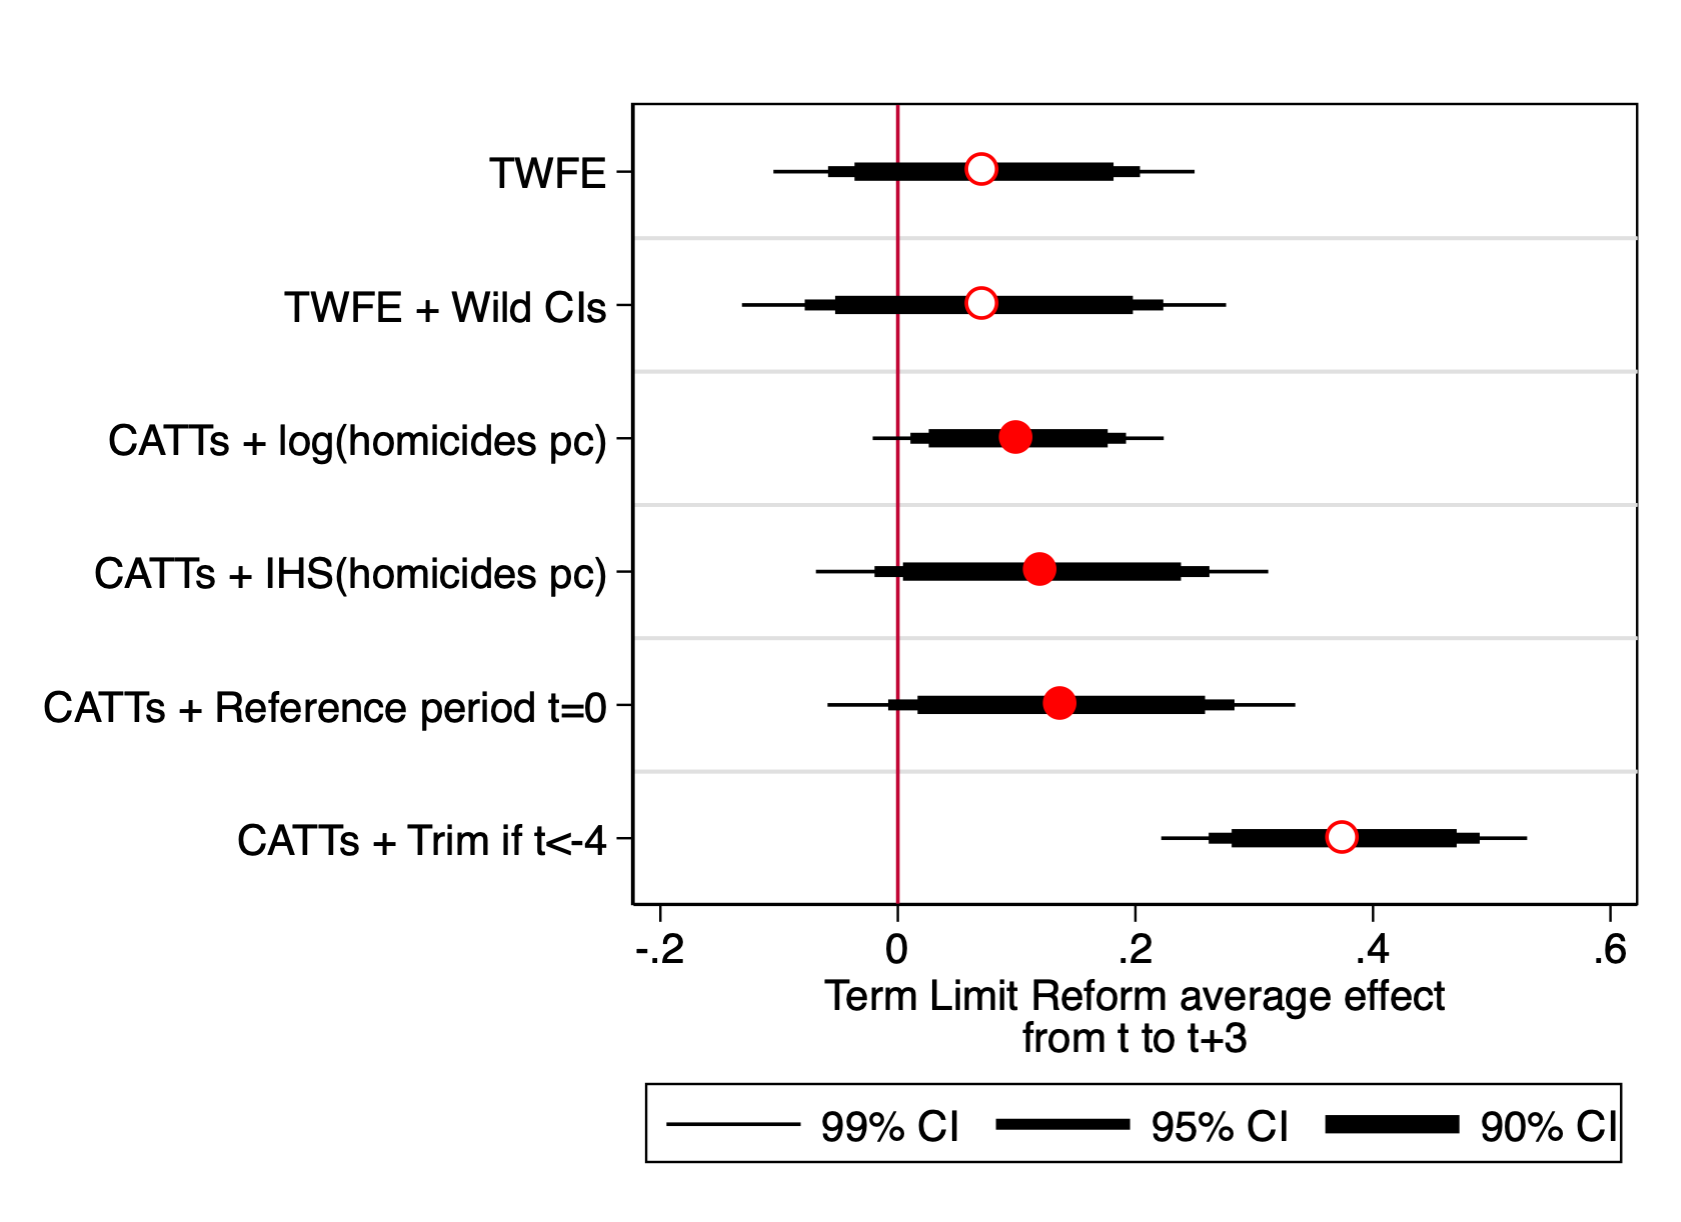
\includegraphics[width=0.9\textwidth]{Figures/average_effects_homicides.png}
       \captionsetup{justification=centering}
       
 \textbf{Note:} Figure \ref{fig:robustness_violence} shows the average treatment effect from t to t+3 across multiple specifications. This average effect was estimated using the IW estimators following \citet{abraham_sun_2020} for each lead and lag relative to the first year a municipality implemented reelection. Red points show that parallel trends hold, while hollow ones imply pretrends. 
\end{figure}      
   
\begin{figure}[H] 
\centering
 \caption{Effect of Term Limit Reform on Violence, propensity score matching on pretreatment covariates}
 \label{fig:matching_violence}
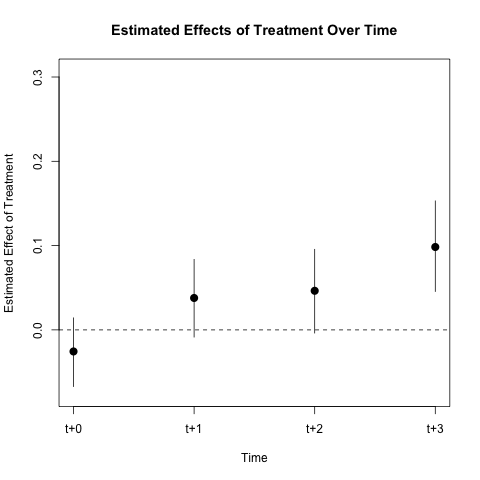
\includegraphics[width=0.75\textwidth]{Figures/panelmatch_logdefuncionespc.png}
       \captionsetup{justification=centering}
    
        
 \textbf{Note:} Figure \ref{fig:matching_violence} produced by propensity score matching that adjust for the treatment and covariate histories during the 5 year periods prior to the treatment. I report 95\% bootstrap confidence intervals clustered at the state level. Covariates include those used to generate Figure \ref{fig:event_study_agreements}. 
 
\end{figure}   
           
    
    
 \clearpage   
 
 %%%% NO ANTICIPATORY ASSUMPTION   
\section{Validating the no-anticipatory assumption \label{appendix:CDLZ}}

\renewcommand{\thetable}{C-\arabic{table}}
\setcounter{table}{0}
 \renewcommand{\thefigure}{C-\arabic{figure}}
\setcounter{figure}{0}
    
         
One way to address the no-anticipatory behavior is to assume that it can only occur in a fixed window prior to the electoral reform, say of one year, especially since the reform was announced in early 2013. However, for states that implemented reelection later this fixed window assumption would not suffice. In other words, only those early adopters of the reform would show unbiased estimates. Late adopters, however, would anticipate the term limit removal an act accordingly biasing the results upwardly.  
 
Another way to assess the no-anticipatory behavior from incumbents in this setting is test whether early vs late adopters differed in their estimated effects. Appendix Figure \ref{fig:CDLZ_agreements} presents \citet{cengiz_etal_2019} ``event-by-event analysis" that estimates treatment effects for each treated Mexican state (28 states) in the sample. States color differs if they are early (2015, red color) or late adopters (2016-2018, blue color). Specifically, I create state-event specific panel datasets and estimate state-specific estimates using separate regressions for each state. Each state dataset contains the treated state and all other states that never received treatment or received treatment after the sample window of $t+1$. For each state I estimate the following DiD regression: 
   
\begin{equation}
y_{mt}=\mu_m	 + \mu_t + \gamma Reform_{mt} + \epsilon_{mt}
\end{equation}

where $Reform_{mt}$ is an indicator variable that takes the value of 1 if the state implemented reelection. If there was evidence of strong incumbent anticipatory behavior, conditional on state covariates such as governor winning margin and alignment with Federal Executive, we would expect strong color clustering across similar estimated effects. In other words, if there is an endogenous response by states to implement the electoral reform, we would see that the positive (or negative) treatment effect would be only by those that implemented reelection earlier or later (events with the same color would be clustered). However, as seen in Appendix Figure \ref{fig:CDLZ_agreements}, this is not the case: there is wide variation in estimated coefficients across early (red) and late (blue) adopters of the reform, conditional and unconditional on state covariates. One would be concerned of the five blue states clustered in the positive end. However, if there was anticipation in these states they would only represent a downward bias of the main results found on the paper.  

\begin{figure}[h]
\centering
\caption{``Event-by-event analysis'' following \citet{cengiz_etal_2019}\\ -95\% confidence intervals-} 
\label{fig:CDLZ_agreements}
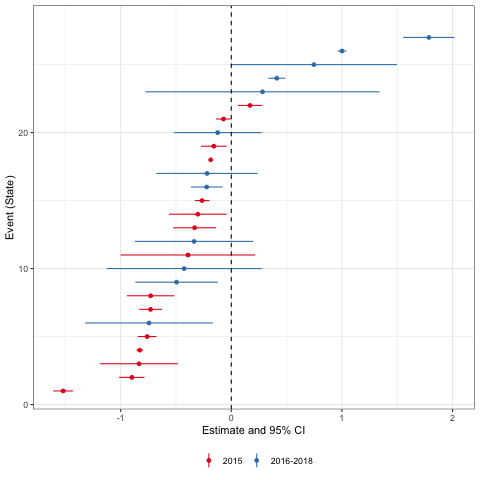
\includegraphics[width=0.5\textwidth]{Figures/CDLZ_cov_acuerdo.png}
       \captionsetup{justification=centering}
       \\
 {\textbf Note:} Estimate separate treatment effects for each event, i.e. each Mexican state in the sample. Each event dataset contains the treated state and all other states that never received treatment or received treatment after the sample window ($t+1$).   
\end{figure}     
   
For robustness, Appendix Figure \ref{fig:stacked_wcontrols_agreements} presents the ``stacked dataset analysis" from \citet{cengiz_etal_2019}. I take each of the ``event-by-event'' datasets from the Appendix Figure \ref{fig:CDLZ_agreements}, stack estimates by cohort and estimate one set of lead and lag variables not using prior treated units as controls. Appendix Figure \ref{fig:stacked_wcontrols_agreements} shows that conditional on state-level covariates, there is strong evidence of parallel trends as well as negative effect of reelection on delegation, but noisy.
       
    
\begin{figure}[H]
\centering
\caption{``Stacked dataset analysis'' following \citet{cengiz_etal_2019}\\ -95\% confidence intervals-} 
\label{fig:stacked_wcontrols_agreements}

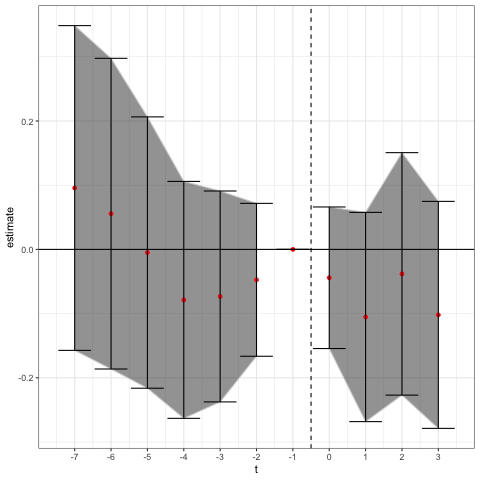
\includegraphics[width=0.5\textwidth]{Figures/stacked_dataset_wcontrols_acuerdo.png}
       \captionsetup{justification=centering}
       \\
 {\textbf Note: Utilize estimated coefficients from Figure \ref{fig:CDLZ_agreements} and stack them in relative time, and estimate lead and lag variables to treatment following the event-by-event analysis setup, i.e. without treatment containment from using prior treated units of controls. Analysis done stacking at the cohort level, and adding municipality and year fixed effects, and clustered standard errors at the state level.}     
\end{figure}   


\clearpage
   
%%%%%%%%%%%%%%%%%%%%%%%%%%%%%%%%% 

  
\end{document}
